%%%%%%%%%%%%%%%%%%%%%%%%%%%%%%%%%%%%%%%%%%%%%%%%%%%%%%%%%%%%%%%%%
%
%   Template para monografia de TCC-2022 - versao 1.0.alfa
%
%%%%%%%%%%%%%%%%%%%%%%%%%%%%%%%%%%%%%%%%%%%%%%%%%%%%%%%%%%%%%%%%%
%%
%% Este template utiliza o modelo mantido pela abnt e foi baseado 
%% no abtex2-modelo-trabalho-academico.tex, v-1.9.6 laurocesar
%% Copyright 2012-2016 by abnTeX2 group at http://www.abntex.net.br/ 
%%
% -------------------------------------------------------------------
%% This work may be distributed and/or modified under the conditions 
%% of the LaTeX Project Public License, either version 1.3 of this 
%% license or (at your option) any later version. The latest version 
%% of this license is in http://www.latex-project.org/lppl.txt
%% and version 1.3 or later is part of all distributions of LaTeX
%% version 2005/12/01 or later.
%%
%% This work has the LPPL maintenance status `maintained'.
%% 
%% The Current Maintainer of this work is the abnTeX2 team, led
%% by Lauro César Araujo. Further information are available on 
%% http://www.abntex.net.br/
%%
%% This work consists of the files abntex2-modelo-trabalho-academico.tex,
%% abntex2-modelo-include-comandos and abntex2-modelo-references.bib
% -------------------------------------------------------------------
%%
%% Modelo de Monografia em conformidade com ABNT NBR 14724:2011
%%
%%%%%%%%%%%%%%%%%%%%%%%%%%%%%%%%%%%%%%%%%%%%%%%%%%%%%%%%%%%%%%%%%
%%
%% ATENÇAO para as opções:
%%
%% para modo rascunho, sem páginas brancas, use: 
%% openany, oneside, nopartblankpage
%%
%% para modo normal, com tudo que ABNT exige, use:  
%% openright, twoside, partpageblank
%%

\documentclass[
	% -- opções da classe memoir --
	12pt,			% tamanho da fonte
	openany,		% capítulos começam em qq página (isso elimina várias pág brancas)
	%openright,		% capítulos começam em pág ímpar (insere página vazia caso preciso)
	oneside,		% considera impressão de um só lado (gera menos pág brancas)
	%twoside,		% para impressão em recto e verso. Oposto a oneside
	a4paper,		% tamanho do papel. 
	% -- opções da classe abntex2 --
	%chapter=TITLE,		% títulos de capítulos convertidos em letras maiúsculas
	%section=TITLE,		% títulos de seções convertidos em letras maiúsculas
	%subsection=TITLE,	% títulos de subseções convertidos em letras maiúsculas
	%subsubsection=TITLE,% títulos de subsubseções convertidos em letras maiúsculas
	% -- opções do pacote babel --
	english,		% idioma adicional para hifenização
	%french,		% idioma adicional para hifenização
	%spanish,		% idioma adicional para hifenização
	%portuges		% o último idioma é o principal do documento
	brazil			% o último idioma é o principal do documento
	]{abntex2}


% ------------------------------------------------------------------------
%   Componente do template para monografia de TCC-2018 - versao 1.0.alfa
% ------------------------------------------------------------------------

%------------ Pacotes básicos 
\usepackage{lmodern}			% Usa a fonte Latin Modern	
\usepackage[table,xcdraw]{xcolor}
\usepackage{tabularx,ragged2e}
\newcolumntype{C}{>{\arraybackslash}X}
\usepackage[T1]{fontenc}		% Selecao de codigos de fonte.
\usepackage[utf8]{inputenc}		% Codificacao do documento (conversão automática dos acentos)
\usepackage{lastpage}			% Usado pela Ficha catalográfica
\usepackage{indentfirst}		% Indenta o primeiro parágrafo de cada seção.
\usepackage{color}			% Controle das cores
\usepackage{graphicx}			% Inclusão de gráficos
\usepackage{microtype} 			% para melhorias de justificação
%------------ Pacotes adicionais
\usepackage{blindtext}			% para geração de dummy text
\usepackage{subcaption}
\usepackage{caption}
\usepackage{longtable}


%------------ Pacotes de citações
\usepackage[brazilian,hyperpageref]{backref}	% Paginas com as citações na bibl
\usepackage[alf]{abntex2cite}		% Citações padrão ABNT
\usepackage{pdfpages}			% Saida em pdf

%------------ Comandos úteis
\newcommand{\aspas}[1]{``#1''}

% ----- PACOTE
\usepackage{listings}
\usepackage{color}
\usepackage{xcolor,xparse}
\usepackage{realboxes}
\usepackage[brazil]{babel}
\usepackage[utf8]{inputenc}

\newcolumntype{b}{X}
\newcolumntype{s}{>{\hsize=.25\hsize}X}
\newcolumntype{d}{>{\hsize=.5\hsize}X}

\definecolor{dkgreen}{rgb}{0,0.6,0}
\definecolor{gray}{rgb}{0.5,0.5,0.5}
\definecolor{backcolour}{rgb}{0.95,0.95,0.95}
\definecolor{mauve}{rgb}{0.58,0,0.82}
\definecolor{darkblue}{rgb}{0.0,0.0,0.6}
\definecolor{cyan}{rgb}{0.0,0.6,0.6}

\lstset{frame=tb,
  backgroundcolor=\color{backcolour}, 
  aboveskip=3mm,
  language=php,
  belowskip=3mm,
  showstringspaces=false,
  columns=fullflexible,
  basicstyle=\ttfamily,
  numbers=none,
  numberstyle=\tiny\color{gray},
  keywordstyle=\color{blue},
  commentstyle=\color{dkgreen},
  stringstyle=\color{mauve},
  breaklines=true,
  breakatwhitespace=true,
  tabsize=3
}

\lstdefinelanguage{XML}
{
  morestring=[b]",
  morestring=[s]{>}{<},
  morecomment=[s]{<?}{?>},
  stringstyle=\color{black},
  identifierstyle=\color{mauve},
  keywordstyle=\color{cyan},
  morekeywords={xmlns,version,type}% list your attributes here
}

\lstdefinestyle{small}
{
}

\renewcommand{\lstlistingname}{Código}

\DeclareDocumentCommand{\clist}{v}{%
    \Colorbox{backcolour}{\csname lstinline\endcsname!#1!}%
}

% ----------- CONFIGURAÇÕES DE PACOTES
%lista de codigos
\renewcommand\lstlistlistingname{Lista de códigos}

% Configurações do pacote backref
% Usado sem a opção hyperpageref de backref
\renewcommand{\backrefpagesname}{Citado na(s) página(s):~}
% Texto padrão antes do número das páginas
\renewcommand{\backref}{}
% Define os textos da citação
\renewcommand*{\backrefalt}[4]{
	\ifcase #1 %
		Nenhuma citação no texto.%
	\or
		Citado na página #2.%
	\else
		Citado #1 vezes nas páginas #2.%
	\fi}%
% ---

% Espaçamentos entre linhas e parágrafos 
% O tamanho do parágrafo é dado por:
\setlength{\parindent}{1.3cm}
% Controle do espaçamento entre um parágrafo e outro:
\setlength{\parskip}{0.2cm}  % tente também \onelineskip

% compila o indice
\makeindex

% Configuração de posicionamento padrão:
\setfloatlocations{quadro}{hbtp}

% ----------------------------------------------------
% Configurações de aparência do PDF final
% ----------------------------------------------------

% alterando o aspecto da cor azul
\definecolor{blue}{RGB}{41,5,195}

% informações do PDF
\makeatletter
\hypersetup{
     	%pagebackref=true,
		pdftitle={\@title}, 
		pdfauthor={\@author},
    	pdfsubject={\imprimirpreambulo},
	    pdfcreator={LaTeX with abnTeX2},
		pdfkeywords={abnt}{latex}{abntex}{abntex2}{trabalho acadêmico}, 
		colorlinks=true,       		% false: boxed links; true: colored links
    	linkcolor=blue,          	% color of internal links
    	citecolor=blue,        		% color of links to bibliography
    	filecolor=magenta,      		% color of file links
		urlcolor=blue,
		bookmarksdepth=4
}
\urlstyle{same}
\makeatother

% ----------------------------------------------------
% Comandos para geração de itens textuais 
% ----------------------------------------------------

\newcommand{\notarodape}[2]{\footnote{Disponível em \url{#1}. Acesso em #2}}

\newcommand{\revisado}[1]{\colorbox{green}{\textbf{#1}}}
\newcommand{\revisar}[1]{\colorbox{yellow}{\textbf{#1}}}

\newcommand{\imprimirfichacatalografica}{

\begin{fichacatalografica}
	\sffamily
	\vspace*{\fill}					% Posição vertical
	\begin{center}					% Minipage Centralizado
	\fbox{\begin{minipage}[c][8cm]{14.0cm}		% Largura
	\small
	
	\hspace{1cm} \imprimirautor\\

	\begingroup
        \leftskip4em
        \rightskip\leftskip
	
	\imprimirtitulo  / \imprimirautor. -- \imprimirlocal, \imprimirdata.
	
	\pageref{LastPage} p. : il. (algumas color.) ; 30 cm.\\
	
	\imprimirorientadorRotulo~\imprimirorientador\\
	
	%\imprimirtipotrabalho~--~\imprimirinstituicao, \imprimirdata.\\
	Monografia para trabalho de conclusão de curso (graduação)~--~Instituto Federal 
	de Educação, Ciência e Tecnologia de Minas Gerais, Ciência da Computação, 
	Formiga, \imprimirdata.\\
	
	1. Certificação Digital.
	2. Assinatura Digital.
	3. Certificado Digital.
	I. \imprimirorientador.
	II. Instituto Federal de Educação, Ciência e Tecnologia de Minas Gerais.
	III. Ciência da Computação.
	IV. \imprimirtitulo 			
        \par
        \endgroup
	\end{minipage}}
	\end{center}
\end{fichacatalografica}

}

\newcommand{\imprimirerrata}{

\begin{errata}
Exemplo de errata\\[1cm]

FERRIGNO, C. R. A. \textbf{Tratamento de neoplasias ósseas apendiculares com
reimplantação de enxerto ósseo autólogo autoclavado associado ao plasma
rico em plaquetas}: estudo crítico na cirurgia de preservação de membro em
cães. 2011. 128 f. Tese (Livre-Docência) - Faculdade de Medicina Veterinária e
Zootecnia, Universidade de São Paulo, São Paulo, 2011.

\begin{table}[htb]
\center
\footnotesize
\begin{tabular}{|p{1.4cm}|p{1cm}|p{3cm}|p{3cm}|}
  \hline
   \textbf{Folha} & \textbf{Linha}  & \textbf{Onde se lê}  & \textbf{Leia-se}  \\
    \hline
    1 & 10 & auto-conclavo & autoconclavo\\
   \hline
\end{tabular}
\end{table}

\end{errata}

}

\newcommand{\imprimirfolhadeaprovacao}[1]{

\begin{folhadeaprovacao}
  \begin{center}
   {\ABNTEXchapterfont\large\imprimirautor}

   \vspace*{\fill}\vspace*{\fill}
   \begin{center}
     \ABNTEXchapterfont\bfseries\Large\imprimirtitulo
   \end{center}
   \vspace*{\fill}
    
   \hspace{.45\textwidth}
   \begin{minipage}{.5\textwidth}
       \imprimirpreambulo
   \end{minipage}%
   \vspace*{\fill}        
   \end{center}
   
   Trabalho aprovado em {#1}.
   
   \vspace{1cm}
   \hspace{4cm} BANCA EXAMINADORA    

   \assinatura{\textbf{\imprimirorientador} \\ Orientador} 
   \assinatura{\textbf{Prof. Dr. Manoel Pereira Júnior} \\ Convidado 1}
    \assinatura{\textbf{Prof. Ms. Fernando Paim Lima} \\ Convidado 2}
   
   %\assinatura{\textbf{Professor} } %\\ Convidado 3}
   %\assinatura{\textbf{Professor} } %\\ Convidado 4}
      
   \begin{center}
    \vspace*{0.5cm}
    {\large\imprimirlocal}
    \par
    {\large\imprimirdata}
    \vspace*{1cm}
  \end{center}
  
\end{folhadeaprovacao}

}
	

\graphicspath{{./figuras/}}   	% pasta contendo todas as figuras

\nopartblankpage  		% elimina páginas em branco
% \partpageblank		% permite páginas em branco

% PACOTES
\usepackage{outlines}
\usepackage{lmodern}
\usepackage[T1]{fontenc}
\usepackage[utf8]{inputenc}
\usepackage{lastpage}
\usepackage{pgfplots}
\usepackage{indentfirst}
\usepackage{color}
\usepackage{graphicx}
\usepackage{microtype}
% \renewcommand\thesection{\arabic{section}}
\usepackage[brazilian,hyperpageref]{backref}
\usepackage[alf]{abntex2cite}
\usepackage{float}
\usepackage{amsmath}
\usepackage{svg}
\svgpath{{../figuras/}}
% ----------------------------------------------------
% Informações de dados para CAPA e FOLHA DE ROSTO
% ----------------------------------------------------

\titulo{Protótipo de uma aplicação web para gestão de eventos online}
\autor{Nikollas Ferreira Gonçalves}
\local{Formiga - MG}
\data{2022}
\orientador{Me. Roger Santos Ferreira}
%\coorientador{Dr. Manoel Pereira Júnior}
\instituicao{%
  Instituto Federal de Educação, Ciência e Tecnologia de Minas Gerais \par
  Campus Formiga \par
  Ciência da Computação
  }
\tipotrabalho{Monografia}
% O preambulo deve conter o tipo do trabalho, o objetivo, o nome da instituição e a área de concentração 
\preambulo{Monografia do trabalho de conclusão de curso apresentado ao Instituto 
    Federal Minas Gerais - Campus Formiga, como requisito parcial para a obtenção 
    do título de Bacharel em Ciência da Computação.}

% ----------------------------------------------------
% INÍCIO DO DOCUMENTO
% ----------------------------------------------------

\begin{document}

%\selectlanguage{portugues}
\selectlanguage{brazil}

\frenchspacing  % retira espaço extra obsoleto entre as frases.

%-----------------------------------------------------
% ELEMENTOS PRÉ-TEXTUAIS
%-----------------------------------------------------
% \pretextual

\imprimircapa

\imprimirfolhaderosto*  % o comando com * indica que haverá ficha bibliográfica

%------------- Ficha catalográfica
% São os ``Dados internacionais de catalogação-na-publicação''.
% Escolha uma das opções: usar página pdf pronta (gerada pela biblioteca!!!)
% ou gerar a página com o comando \imprimirfichacatalografica. 
% (Mais detalhes no preludio e documentacao do pacote abntex2.)
%
 \begin{fichacatalografica}
     %\includepdf{ficha_catalografica.pdf}
 \end{fichacatalografica}
%\includepdf{anexos/ficha.pdf} %use esta linha quando tiver o PDF com a ficha catalográfica gerada pela biblioteca

%------------ Errata (se houver)
% Modifique o comando \imprimirerrata no preludio e use esse comando
%\imprimirerrata

%------------ Folha de aprovação
% É um elemento obrigatório da NBR 14724/2011 (seção 4.2.1.3). 
% Você pode utilizar a página modelo até a aprovação do trabalho. 
% Após isso, gere uma página com a imagem da folha assinada pela banca,
% comente o comando \imprimirfolhadeaprovacao e use o \includepdf
% \includepdf{folhadeaprovacao_final.pdf}
\newpage
%------------ Dedicatória
\begin{dedicatoria}
  \vspace*{\fill} \centering \noindent 
  \textit{Dedico este trabalho a minha família,  pois é graças ao seu incentivo que hoje pude concluir o meu curso.} 
  \vspace*{\fill}
\end{dedicatoria}

%------------ Agradecimentos
\begin{agradecimentos}
Agradeço a todos que estiveram presentes nos momentos de dificuldade desta monografia, deste curso, em especial minha família que me apoiou constantemente nesta jornada.
\end{agradecimentos}

%------------ Epígrafe
\begin{epigrafe}
   \vspace*{\fill}
   \begin{flushright}
	\textit{\aspas{As máquinas me surpreendem muito frequentemente.} \\
	(Alan Turing) }
   \end{flushright}
\end{epigrafe}

%------------ RESUMOS
\setlength{\absparsep}{18pt} % ajusta o espaçamento dos parágrafos do resumo

% resumo em português
\begin{resumo}
Com o aumento da demanda por eventos online nos últimos anos, foram necessários adotar métodos que antes não eram utilizados, como aplicações gerenciadoras de eventos. O presente trabalho apresenta um protótipo de uma aplicação web com o propósito de gerir os eventos, utilizando-se de \textit{frameworks} modernos, como o Next.js para o desenvolvimento do frontend e o Laravel para o backend. A distribuição vertical se deve à aplicação ser dividida logicamente em dois servidores distintos, que melhora o gerenciamento de sua arquitetura. Com estes recursos e seu planejamento com a metodologia unificada, o protótipo final apresenta a implementação por meio das tecnologias citadas, além de exemplificar o uso dos conceitos almejados no desenvolvimento de aplicações web atualmente: design responsivo e fluído, além de demonstrar a divisão de responsabilidades entre as camadas de software.

\textbf{Palavras-chave}: Laravel, Gerenciamento de eventos, Next.js
\end{resumo}

% resumo em inglês
\begin{resumo}[Abstract]
\begin{otherlanguage*}{english}
With the increase in demand for online events in recent years, it was necessary to adopt methods that were not used before, such as event management applications. The current work presents a prototype of a web application with the purpose of managing events, using modern frameworks, like Next.js for the frontend development and Laravel for the backend. The vertical distribution is due to the application being logically divided into two distinct servers, which improves the management of its architecture. With these resources and it's planning with the unified methodology, the final prototype presents the implementation through the mentioned technologies, in addition to exemplifying the use of the desired concepts in the development of web applications today: responsive and fluid design, in addition to demonstrating the division of responsibilities between software layers.

\textbf{Keywords}: Laravel, Event management, Next.js
\end{otherlanguage*}
\end{resumo}
 


% Consulte o manual da classe abntex2 para maiores 
% orientações sobre os seguintes tópicos:

%------------ Lista de ilustrações
\pdfbookmark[0]{\listfigurename}{lof}
\listoffigures*
\cleardoublepage

%------------ Lista de tabelas
%\pdfbookmark[1]{Lista de tabelas}{lof}
%\listoftables*
%\cleardoublepage

%------------ Lista de códigos
\pdfbookmark[2]{Lista de códigos}{lof}
\addcontentsline{toc}{chapter}{\lstlistlistingname}
\newlistof{lstlistoflistings}{lol}{\lstlistlistingname}
\lstlistoflistings*
\cleardoublepage


%------------ Lista de abreviaturas e siglas
\begin{siglas}
    \item[HTML] \textit{Hyper Text Markup Language}
    \item[CSS]  \textit{Cascade Style Sheet}
    \item[JS]   \textit{JavaScript}
    \item[TS]   \textit{TypeScript}
    \item[PHP]  \textit{PHP: Hypertext Preprocessor}
    \item[JSON] \textit{JavaScript Object Notation}
    \item[JWT]  \textit{JSON Web Token}
    \item[ORM]  \textit{Object Relational Mapper}
    \item[SQL]  \textit{Structured Query Language}
    \item[API]  \textit{Application Programming Interface}
    \item[SGBD] \textit{Sistema Gerenciador de Banco de Dados}
    \item[PU]   \textit{Processo Unificado}
    \item[CDN] \textit{Content Delivery Network}
    \item[IHC] \textit{Interface Humano Computador}
\end{siglas}
%------------ Lista de símbolos

%------------ Sumario
\pdfbookmark[0]{\contentsname}{toc}
\tableofcontents*
\cleardoublepage

% ----------------------------------------------------------
% ELEMENTOS TEXTUAIS
% ----------------------------------------------------------
\textual

%inclua outros capítulos de acordo com a orientação do seu professor
% ----------------------------------------------------------
\chapter{Introdução}
\label{chp:LABEL_CHP_1}

% ----------------------------------------------------------

Segundo o \citeonline{Sebrae}, em abril de 2020, a pandemia do covid-19 afetou 98\% do setor de eventos, devido a cancelamentos, renegociações, entre outros motivos para evitar aglomerações. Destes eventos afetados, muitos empresários estão se preocupando com aprimorar sua gestão, e conforme o site feiras do Brasil o número de eventos online para 2021 já supera o número presencial devido à alta demanda. Além disso, de acordo com estudo da Associação Brasileira de Promotores de Eventos (Abrape), 51,9\% dos eventos previstos para ocorrer neste período foram cancelados ou adiados \cite{FEIRA}.

Para que estes eventos sejam realizados de uma forma mais eficiente, utilizam-se diversas ferramentas online que possibilitam o gerenciamento de eventos remotos e presenciais, entre essas:
\begin{itemize}
    \item \textbf{Even3: }O Even3 é uma plataforma online a qual disponibiliza espaço para que instituições e/ou organizações criem seus próprios eventos e os hospedem, neste também é possível a criação de eventos gratuitos e pagos, além da emissão de certificados. E dito isso, segundo o site do Reclame Aqui, o maior problema deles é sua emissão de certificado, que apresenta problemas por parte da própria aplicação.
    \item \textbf{OCS:} O Open Conference System é um \textit{software} que teve seu desenvolvimento paralisado pela equipe, e que possui seu código aberto onde o usuário pode elaborar o seu próprio site de compartilhamento de conferências acadêmicas. Este processo é realizado manualmente, como a página do site, por exemplo, mas há exceções do que vem fornecido pelo sistema, o cadastro de participantes, por exemplo.
    \item \textbf{Sympla: }O Sympla é uma plataforma, similar ao Even3, que se propõe a gestão completa e otimizada através de dezenas de ferramentas simples de usar, com eventos gratuitos e pagos também, além de shows e eventos. Seu maior problema, segundo a sua página no Reclame Aqui, é no quesito de ingressos, principalmente em sua compra e recebimento.
    \item \textbf{EventBrite: }O Eventbrite é uma plataforma global de ingressos de autoatendimento para experiências ao vivo que permite a qualquer pessoa criar, compartilhar, encontrar e participar de eventos, festivais, maratonas e conferências, entre outros. Mas grande parte de seus problemas também se dão na compra e recebimento de ingressos, de acordo com reclamações de sua página no Reclame Aqui.
    \item \textbf{S-EVA: }O S-EVA (Sistema de Eventos Acadêmicos) é um protótipo que implementa a solução de eventos acadêmicos, no qual o seu foco é utilizar um banco de dados integrado a um \textit{framework} para interface gráfica, além de avaliar trabalhos correlatos e destacar pontos importantes sobre gestão de eventos.
\end{itemize}

% As quatro primeiras soluções são encontradas diretamente no mercado e estão prontas para o uso, porém o S-EVA foi feito como um protótipo em 2016 por meio de um projeto acadêmico.

% O propósito deste trabalho de conclusão de curso (TCC) é criar um protótipo de aplicação web que gerencie eventos acadêmicos de forma que possua uma conceitos almejados no desenvolvimento de aplicações web atualmente: design responsivo, fluído, tendo um foco na User Interface e User Experiencie, além de demonstrar a divisão de responsabilidades entre as camadas de \textit{software} por meio do padrão de desenvolvimento MVC e programação reativa.

% ----------------------------------------------------------
% JUSTIFICATIVA
% ----------------------------------------------------------

\section{Justificativa}

Aplicar os conceitos aprendidos teoricamente em cursos de tecnologia da informação, como Sistemas de Informação, Engenharia da Computação e principalmente a Ciência da Computação, visando um design fluído, com boas práticas de IHC, a modelagem de banco de dados onde a implementação de uma metodologia de desenvolvimento e projeto para a aplicação proposta por meio de \textit{frameworks} modernos.

% ----------------------------------------------------------
% OBJETIVOS
% ----------------------------------------------------------

\section{Objetivos}
O objetivo geral deste trabalho de conclusão de curso é desenvolver um protótipo de uma aplicação web para gerenciar eventos acadêmicos online, exemplificando o uso de conceitos almejados no desenvolvimento de aplicações web atualmente. 


\begin{itemize}
    \item Modelar a arquitetura do sistema.
    \item Implementação do modelo de banco de dados.
    \item Desenvolvimento da camada de \textit{backend} em Laravel.
    \item Desenvolvimento da camada de \textit{frontend} em Next.js.
    \item Implementação do funcionamento do gerenciador de eventos.
\end{itemize}

% ----------------------------------------------------------
% ESTRUTURA DO TRABALHO
% ----------------------------------------------------------
\section{Estrutura do trabalho}

Este trabalho está dividido em seis capítulos. O capítulo \ref{chp:LABEL_CHP_2} apresenta o referencial teórico. O capítulo \ref{chp:LABEL_CHP_3} expõe a metodologia.
No capítulo \ref{chp:LABEL_CHP_4} é retratado o desenvolvimento. No capítulo \ref{chp:LABEL_CHP_5} são apresentados os resultados obtidos. Por fim, no capítulo \ref{chp:LABEL_CHP_6} são feitas as
considerações finais e trabalhos futuros, seguidas pelas referências bibliográficas.
% ----------------------------------------------------------
\chapter{Fundamentação Teórica}\label{chp:LABEL_CHP_2}
% ----------------------------------------------------------
Para entendimento da aplicação da monografia que será apresentada, são necessários alguns conceitos. Por se tratar de uma aplicação web, primeiramente é preciso definir os conceitos do planejamento e estruturação, por meio da engenharia de software, o conceito de frontend, que é a interface da aplicação com o usuário, o backend, onde é feito o tratamento das informações com o banco de dados.

\section{Engenharia de Software}\label{engsoft}
A tendência é que softwares fiquem cada vez maiores e mais complexos, e isto se deve ao poder computacional crescente a cada ano. E isto faz com que os usuários criem maiores expectativas em relação aos sistemas de software, que não apenas devem transmitir informações pela internet de forma rápida e segura, mas também adaptados à necessidade de quem o usa. \cite{SOMMERVILE}.

A engenharia de software abrange os processos com um conjunto de métodos e diversas ferramentas que possibilitam aos profissionais desenvolverem sistemas de software com melhor planejamento \cite{PRESSMAN}. Tendo técnicas as quais irão se construir com base na especificação, projeto e evolução dos programas, que normalmente não são relevantes para o primeiro estágio de qualquer processo de projeto de software é o desenvolvimento de uma compreensão dos relacionamentos entre o software que está sendo projetado e seu ambiente externo. E isto é essencial para decidir qual funcionalidade o sistema terá e poderá ser apresentada ao usuário final, assim como a estruturação do próprio projeto e principalmente estabelecer os limites do sistema, ou seja, até que ponto será desenvolvido baseado no contexto do software \cite{SOMMERVILE}.

Para que isso seja planejado em uma aplicação e utilizada corretamente, de acordo com \cite[p.126]{SOMMERVILE}: \begin{quote}
    “Modelos de contexto do sistema e modelos de interação apresentam visões complementares dos relacionamentos entre um sistema e seu ambiente.”
\end{quote} 
\subsection{Caso de uso}
Segundo \citeonline{PRESSMAN}, a UML é uma linguagem padrão para descrever e documentar um projeto de software que reúne diversos grupos de notações de modelagem, sendo cada um com sua devida sintaxe e semântica predeterminadas. Cada um desses elementos pode ser extensível, permitindo, deste modo, que sejam adaptáveis às características específicas do projeto a ser desenvolvido. A UML independe de linguagem de programação, framework e dos processos de desenvolvimento do software, fazendo com que diferentes abordagens possam ser utilizadas durante o processo \cite{BEZERRA}.

O diagrama UML de caso de uso determina as funcionalidades e características presentes no software sendo uma visão geral do ponto de vista do usuário que descreve como este irá interagir com o sistema, seguindo determinadas ações para realizar um objetivo, como por exemplo fazer um login. Há uma padronização em seu desenvolvimento, representada pelas seguintes características, segundo \citeonline{PRESSMAN} e \citeonline{SOMMERVILE}:
\begin{itemize}
    \item \textbf{Ator: }representado por figuras de um boneco palito, é aquele que irá interagir com o sistema, sendo este externo ao sistema desenvolvido.
    \item \textbf{Caso de uso: }representado por uma elipse no diagrama, estes demonstram as ações que os atores podem realizar dentro do sistema, ou seja, identificam as interações individuais entre o sistema e seus usuários. 
    \item \textbf{Sistema: }elemento opcional representado por um retângulo para definir o objetivo de cada parte do diagrama de caso de uso, sendo 
\end{itemize}

\subsection{Processo unificado}
O processo unificado é um modelo incremental e iterativo derivado de trabalhos sobre a UML que ilustra as práticas na especificação, no projeto e prevê a prototipação aliada a entrega incremental do desenvolvimento. o PU é descrito em cima de três perspectivas, que podem ser descritas como dinâmica, que mostra as fases do modelo ao longo do tempo, estática, que mostra as atividades realizadas no processo e prática, que sugere boas práticas a serem usadas durante o processo \cite{SOMMERVILE}.

Segundo \citeonline{BEZERRA} existem cinco fases do PU, sendo estas:
\begin{itemize}
    \item \textbf{Fase de concepção: }identifica as entidades externas que irão interagir com o sistema, descrevendo os requisitos do projeto, que se desenvolve todo o planejamento para que seja possível as futuras iterações incrementais do processo. Nesta etapa é desenvolvido, também, a arquitetura provisória do sistema, que será refinada e expandida nos processos subsequentes.
    \item \textbf{Fase de elaboração: }refina e expande, por meio da ampliação da arquitetura do sistema, a fase de concepção, criando o modelo de requisitos e o modelo de implementação, mesmo ainda não oferecendo os recursos necessários para a utilização do sistema. Define-se as tecnologias que serão utilizadas ao longo do projeto, como frameworks e banco de dados, por exemplo.
    \item \textbf{Fase de construção: }é a fase que será desenvolvido o sistema por meio da programação, ou seja, as iterações desta etapa serão constituídas por fazer uma parte do sistema e a integrar as demais existentes, podendo serem desenvolvidas em paralelo. Tudo isto deve ser feito seguindo as documentações geradas nesta etapa e nas anteriores, para que não haja falha na entrega dos requisitos necessários. E ao fim desta fase, deve-se ter um sistema de software documentado e funcionando corretamente em seu ambiente operacional, de modo que já possa ser utilizado em modo de teste pelo usuário.
    \item \textbf{Fase de transição: }é a fase que entrega-se o software ao usuário final para testes, juntamente aos manuais de utilização e instalação, se for o caso, fazendo com que sejam relatados possíveis defeitos e ajustes necessários. Na conclusão desta etapa, o software poderá operar em modo de produção.
    \item \textbf{Fase de produção: }disponibiliza o ambiente operacional ao usuário, monitorando o seu uso contínuo, por meio de suporte ao ambiente operacional, realizando alterações e correções se forem necessários.
\end{itemize}

No PU, a iteração ocorre de duas formas: entre as cinco fases e entre a própria fase, fazendo com que possam acontecer de maneira concorrente e escalonada. Pode-se retornar a cada uma dessas etapas caso seja necessário complementar e/ou corrigir algum requisito ou definir uma nova integração, por exemplo, tornando-se incremental a cada etapa.


\section{Padores de projetop}

Padrões de projeto
Os padrões de projeto foram obtidos a partir das ideias apresentadas por Christopher Alexander (ALEXANDER
et al., 1977), que sugeriu haver padrões comuns de projeto de prédios que eram inerentemente agradáveis e
eficazes. O padrão é uma descrição do problema e da essência de sua solução, de modo que a solução possa ser
reusada em diferentes contextos. O padrão não é uma especificação detalhada. Em vez disso, você pode pensar
nele como uma descrição de conhecimento e experiência, uma solução já aprovada para um problema comum.
Uma citação do site da Hillside Group (<http://hillside.net:>), dedicado a manter informações sobre os padrões,
sintetiza seu papel no reúso:
Padrões e Linguagens de Padrões são formas de descrever as melhores práticas, bons projetos e capturar a experiência
de uma forma que torne possível a outros reusaressa experiência.
Os padrões tiveram um enorme impacto no projeto de software orientado a objetos. Além de serem soluções
já testadas para problemas comuns, tornaram-se um vocabulário para falar sobre um projeto. Você pode, portanto,
explicar seu projeto por meio de descrições dos padrões que você usou. Isso é particularmente verdadeiro para os
padrões de projeto mais conhecidos que foram originalmente descritos pela 'Gangue dos Quatro'em seu livro de
padrões (GAMMA et al., 1995). Outras descrições de padrões particularmente importantes são as publicadas em
uma série de livros de autores da Siemens, uma grande empresa europeia de tecnologia (BUSCHMANN et al., 1996;.
BUSCHMANN et al., 2007a; BUSCHMANN et al., 2007b; KIRCHER e JAIN, 2004; SCHMIDT et al., 2000).
Os padrões de projeto são normalmente associados com projeto orientado a objetos. Muitas vezes, os padrões
publicados contam com as características de objetos, como herança e polimorfismo para fornecer generalidade.
No entanto, o princípio geral de encapsular a experiência em um padrão é aquele igualmente aplicável a qualquer
tipo de projeto de software. Então, você poderia ter padrões de configuração para os sistemas COTS. Os padrões
são uma maneira de reusar o conhecimento e a experiência de outros projetistas.
Os quatro elementos essenciais dos padrões de projeto foram definidos pela 'Gangue dos Quatro', em seu livro
de padrões:
1. Um nome que seja uma referência significativa para o padrão.
2. Uma descrição da área de problema que explique quando o modelo pode ser aplicado.
3. A descrição da solução das partes da solução de projeto, seus relacionamentos e suas responsabilidades. Essa
não é uma descrição do projeto concreto; é um modelo para uma solução de projeto que pode ser instanciado
de diferentes maneiras. Costuma ser expresso graficamente e mostra os relacionamentos entre os objetos e

\section{Aplicação web}
Uma aplicação web envolve diversas camadas da programação, lidando desde a interação com o usuário por meio da interface gráfica com o frontend, passando pela maninupulação dos dados com o backend e o seu armazenamento no banco de dados. Isto, deve ser precedido de um planejamento, explicado na seção \ref{engsoft}.

\subsection{Frontend}
O frontend lida com a interface gráfica e apresentação dos dados ao usuário, ou seja, é onde inclui todo o design, estrutura, layout e o conteúdo das páginas que serão exibidas. O \textit{client-side} deve conter boas práticas de User-Interface
\footnote{É mais uma das ferramentas utilizadas para entregar a boa experiência ao usuário, pois é a parte tangível de um projeto, onde você constrói visualmente o site ou qualquer outra plataforma.}
e User-Experience
\footnote{É tudo que envolve o modo como qualquer usuário interage com o mundo ao seu redor. Na verdade o termo user experience é muito amplo, mas quando falamos de marcas, produtos, sistemas e serviços, é importante entender que UX não envolve apenas o design do produto e seu desenvolvimento. Temos que observar todas as etapas do cliente junto à sua marca, desde o primeiro “encontro” até o pós uso ou consumo.} para que o conteúdo seja disposto e melhor interpretado pelo usuário da aplicação. FALTA MELHORAR

\subsubsection{Design responsivo}
A união de técnicas de grids e imagens fluidos, que se adaptam a proporção da tela que está sendo utilizada faz que o design responsivo se torne uma boa prática no desenvolvimento do frontend. A adaptação pode ser apenas o enquadramento de recursos, dada as proporções de altura e largura de uma tela, assim como a reestruturação do layout de forma que os conteúdos sejam exibidos de maneiras distintas nos mais diferentes dispositivos por meio do media query. \cite{MOZILA}

\subsubsection{Programação reativa}
\subsection{Backend}
O backend lida com a manipulação e controle do banco de dados com o foco na parte do servidor de uma aplicação web. Podendo ser utilizado para o gerenciamento de login, nesta camada há a necessidade da proteção dos dados. Os usuários não interagem diretamente com o backend, necessitando de interfaces para realizar tal manipulação.

\subsubsection{API}
A API é um conjunto de rotinas e padrões criados por uma aplicação visando a interoperabilidade entre aplicações. Podendo ser feita na camada de backend, uma API requere uma funcionalidade requisitada por um usuário no frontend para o backend processar os dados e os entregar seguindo um padrão por meio do protocolo HTTP
\footnote{Protocolo cliente-servidor que permite obtenção de recursos, como arquivos JSON ou documentos HTML. É a base da troca de dados pelas aplicações web que suas mensagens são enviadas por meio de requisições e tem como retorno uma resposta.\cite{HTTP}  https://developer.mozilla.org/pt-BR/docs/Web/HTTP/Overview}.
teste
https://becode.com.br/o-que-e-api-rest-e-restful/

\subsection{Framework}
Um framework é um conjunto de ferramentas de programação que fornece funcionalidades genéricas que podem ser alteradas de acordo com o uso específico. Fornecendo um padrão, é possível criar aplicações reunindo estruturas, bibliotecas de código e seu conjunto de ferramentas documentados que estão prontos para o uso do desenvolvedor.

\subsection{Banco de dados relacional}
Segundo \citeonline{HEUSER}, um banco de dados relacional é composto por tabelas ou relações. As tabelas são um um conjunto não ordenado de tuplas, que possuem campos com suas propriedades. As relações, ligam as tabelas entre si por meio de suas chaves, fazendo com que 
\section{Versionamento}
Segundo \citeonline{IPSENSE} o versionamento é uma metodologia aplicada por programadores visando controlar e acompanhar o histórico de alterações em um software, permitindo diferenciar mudanças realizadas em cada versão. A manutenção do código, ou seja adicionar ou alterar informações do sistema para atender novas demandas, pode ser realizada através destas ramificações, que são diferentes instâncias de um mesmo programa, podendo uma instância conter determinadas alterações enquanto a outra se mantém estável sem as modificações \cite{SOMOSTERA}.


https://www.ipsense.com.br/blog/entenda-a-importancia-do-versionamento-de-software/
https://gaea.com.br/entenda-por-que-versionamento-de-software-e-tao-importante/
https://blog.somostera.com/data-science/versionamento

% -----------------------------------------
\chapter{Materiais e Métodos}\label{chp:LABEL_CHP_3}
% -----------------------------------------
\section{Materiais}
FALTA ARRUMAR
\subsection{HTML}
O Hiper Text Markup Language (HTML) é uma linguagem de marcação utilizada para o desenvolvimento de páginas web na qual permite a inserção de conteúdo, estabelece a estrutura básica, assim como a organização de informações de uma página web. Isto o torna o componente básico da web, juntamente ao CSS e JavaScript, sendo um conjunto de elementos conectados formando informações das mais variadas, podendo conter palavras, imagens, documentos entre outros tipos dados. Seu funcionamento se dá pela leitura de seus arquivos, que é renderizada para o usuário final por meio de um navegador web. Portanto, é o esqueleto no qual uma página se forma \cite{FLANAGAN}.
\subsection{CSS}
O Cascading Style Sheets (CSS) é a linguagem utilizada para estilizar o HTML. Isso quer dizer que todos os elementos podem ser estilizados, ou seja, é possível modificar detalhes como espaçamentos, cores, margens, fonte, tamanho desta fonte, bordas, efeitos visuais, entre vários outros detalhes para cada um. Desta maneira, é um complemento ao HTML, dando forma e modificação desta estrutura previamente feita \cite{FLANAGAN}.
\subsection{JavaScript}
JavaScript é a linguagem de programação da web, que é interpretada pelos navegadores web. Diversos sites modernos utilizam esta linguagem para manipular o comportamento da página em conjunto ao HTML e CSS. Podendo ser utilizada tanto no front-end quanto no back-end se torna muito versátil para o desenvolvimento destes sistemas. Além disso, a mudança de dados sem a necessidade de recarregar toda a página permite uma flexibilidade na qual dados podem carregar independentes e de forma assíncrona sem que tenha a necessidade de um usuário final estar constantemente monitorando qualquer alteração \cite{FLANAGAN}.
\subsection{Typescript}
O TypeScript é uma linguagem de programação de código aberto desenvolvido pela Microsoft e é um conjunto de ferramentas e boas práticas de programação para JavaScript, o qual adiciona recursos a esta linguagem. Dentre as adições, vale ressaltar a tipagem estática, visto que JavaScript não suporta isto\cite{TYPESCRIPT}. Além disso, a orientação a objetos também é suportada pelo TypeScript, o que possibilita a criação de interfaces para os objetos. Sua utilização pode ser atrelada ao JavaScript, ou seja, podem ser utilizados em conjunto para uma maior flexibilidade \cite{CHERNY}.
\subsection{PHP}
O PHP é uma linguagem de script open-source de uso geral, muito utilizada, e especialmente adequada para o desenvolvimento web e que pode ser embutida dentro do HTML. Muito utilizada para o back-end, esta linguagem tem evoluído rapidamente, sendo suportada por diversos desenvolvedores ao redor do mundo. Além disso, o PHP moderno engloba muitas práticas novas que podem ser desconhecidas para aqueles que são novos na linguagem ou para aqueles que estão atualizando de suas versões anteriores \cite{LOCKHART}.
\subsection{Laravel}
Framework é um conjunto de ferramentas, recursos e funcionalidades que visa facilitar e agilizar tarefas mais comuns no desenvolvimento de sistemas, e é criado em uma determinada linguagem de. Dito isso, o framework escolhido foi o Laravel, que foi criado no PHP, é gratuito e possui código aberto. Este é utilizado no desenvolvimento de sistemas web e seu objetivo é fornecer código e recursos claros, simples e bonitos que ajudem os desenvolvedores a aprender, iniciar e desenvolver rapidamente e escrever um código simples, claro e duradouro \cite{STAUFFER}. \\
Este framework foi baseado no padrão de projeto Model, View, Controller (MVC), dividindo a aplicação em três camadas, sendo estas o modelo, que dita as regras de negócio assim como os dados da aplicação; o controle, que realiza a interpretação das entradas do usuário, sendo estas convertidas para as demais camadas, ou seja, fazendo uma chamada para o modelo ou convertendo dados para a visão; e visão, que consiste na exibição de dados para o usuário. \\
\begin{figure}[h]
    \caption{\label{framework_popular}Frameworks back-end mais populares}
    \vspace{5pt}
    \centering
    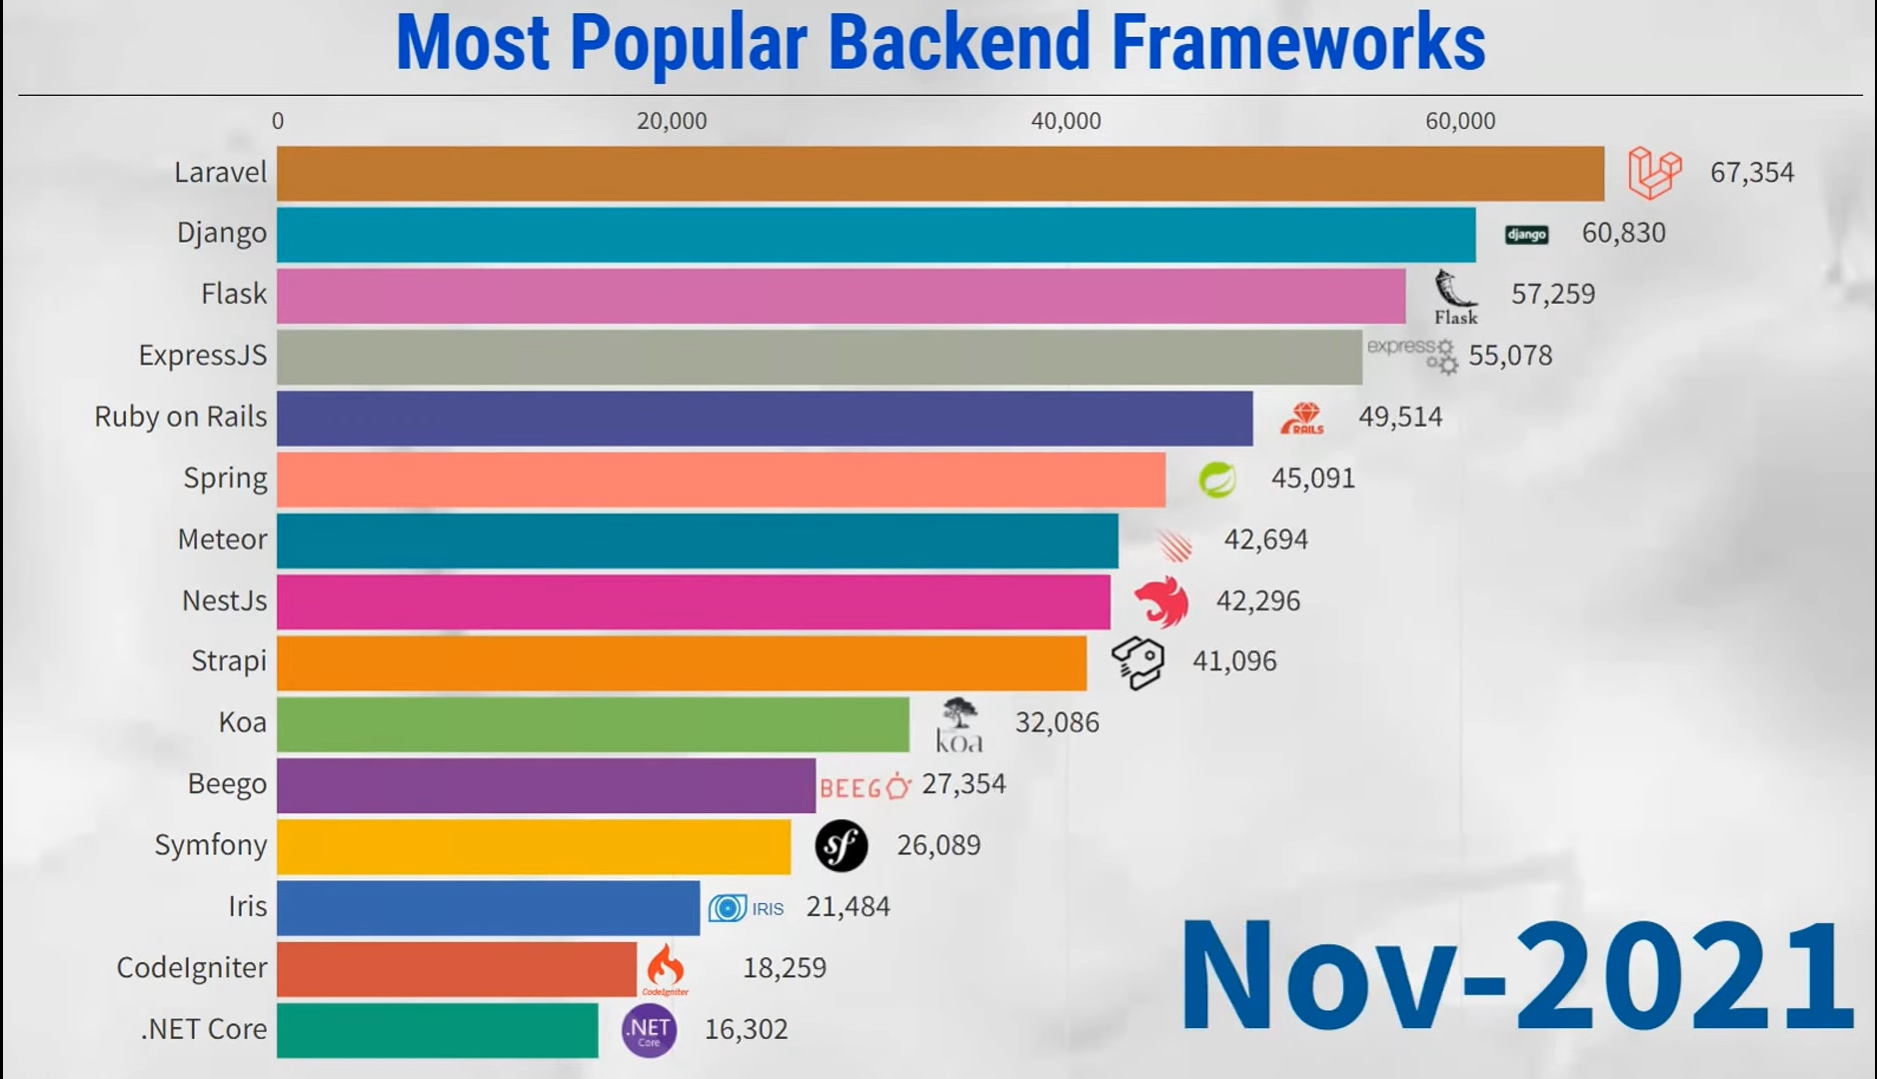
\includegraphics[scale=.20]{laravel.png}
    \vspace{5pt}
    \legend{Fonte: Statistcs and data}
\end{figure}\\
Além disso a escolha para o projeto se deve ao fato de que, de acordo com a figura \ref{framework_popular}, o Laravel é o framework back-end mais popular até março de 2021 segundo dados dos repositórios com mais estrelas do GitHub, e isto se deve a diversas características que estão contidas nele, sendo estas:
\begin{itemize}
    \item \textbf{Roteamento rápido e simples:} é possível criar rotas com segurança e de forma simples, evitando requisições não autorizadas de maneira simples por meio dos verbos GET, POST, PUT e DELETE. Também é possível criar grupos de rotas com permissões de acesso específicas.
    \item \textbf{ORM Eloquent:} este facilita a interação com o banco de dados utilizando cada tabela como um objeto modelo correspondente. Outra facilidade é a forma de interação com as tabelas, que seriam a recuperação de registros do banco de dados, assim como sua inserção, atualização e exclusão.
    \item \textbf{Migration:} As migrations são como o controle de versão do banco de dados, sendo estas as definições de criação e alteração do schema, podendo ser revertidas caso necessário.
    \item \textbf{Transmissão de eventos em tempo real:} utilizando da tecnologia de WebSockets, é possível atualizar em tempo real e constantemente a interface do usuário enviando dados sempre que determinado evento ocorra.
\end{itemize}
\subsection{SQL}
A linguagem SQL é utilizada para executar tarefas em tabelas de banco de dados. Ou seja, com os comandos de inserção, deleção, atualização e leitura de dados é possível manipular as informações por meio de comandos de consulta com diversas informações contidas \cite{HEUSER}. Suas principais características são:
\begin{itemize}
    \item \textbf{Query:} é possível solicitar informações específicas de um banco de dados.
    \item \textbf{Manipulação de dados:} adicionar, excluir, alterar, ordenar, requisitar além outras operações para os registros contidos no banco de dados.
    \item \textbf{Acesso de controle de dados:} fornece técnicas de segurança para proteger dados, limitando quais usuários podem controlar e limitar o que podem fazer com os registros contidos dentro do banco de dados.
\end{itemize}
\subsection{Git}
Controlador de versão é uma ferramenta de software na qual ajuda os desenvolvedores, seja em equipe ou não, a gerenciar alterações no código-fonte, mantendo o registro destas modificações. Então, o GIT é um sistema de controle de versão que possui código aberto, é flexível (possui vários tipos de fluxos de trabalho de desenvolvimento não lineares), é seguro (toda sua estrutura é protegida com um algoritmo de hash de criptografia seguro chamado SHA1) e possui um bom desempenho (Fazer o commit de novas alterações, branches, mesclagem e comparação de versões anteriores – tudo é otimizado para desempenho) \cite{SANTACROCE}.
\subsection{Bootstrap}
Para a estilização do front-end foi escolhido o Bootstrap, que é um framework gratuito de HTML, CSS e JavaScript no qual visa a criação de sites responsivos, ou seja, se adaptando tanto para telas maiores, como monitores de computador assim como para telas menores, como é o caso dos celulares. Além disso, contém bibliotecas prontas de estilização que procuram agilizar o processo de desenvolvimento no CSS e JavaScript, assim como a reutilização do código e sua personalização \cite{SPURLOCK}.

Este possui um sistema de grid, que resultou em sua responsividade, e dimensiona a aplicação em até doze colunas de acordo com o tamanho de cada dispositivo. Além disso possui componentes de interface que agilizam o desenvolvimento, visto que já estão implementados de forma que podem ser personalizados, sendo um exemplo a barra de navegação (navbar).

\subsection{React}
Para melhorar a interatividade da interface do usuário, foi escolhido o React, que segundo seus próprios criados é “uma biblioteca JavaScript declarativa, eficiente e flexível para a criação de interfaces de usuário (UI)”. Isso quer dizer que é uma coleção de funcionalidades que podem ser utilizadas e reutilizadas pelo desenvolvedor, que são seus componentes. Isto permite uma padronização na interface, além de reaproveitamento de código \cite{ZAMMETTI}.

A criação de views é facilitada e simples, sendo estas atualizadas e renderizadas de forma eficiente apenas para os componentes necessários à medida que os dados forem alterados, sendo estas declarativas fazendo que o código seja mais simples de se depurar.

Dito isso, sua forma de trabalhar é com componentes encapsulados gerenciadores dos seus próprios estados, que combinados formam uma UI complexa, podendo ser escritos em JavaScript ou TypeScript.

\subsection{Next.js}
O Next.js é um framework do React, o qual adiciona várias funcionalidades para esta biblioteca, visando acelerar o processo de desenvolvimento. Construído com intuito de melhorar o desempenho da aplicação implementada em React, há uma indexação do conteúdo da página e pelos motores de busca. Ou seja, se torna mais rápido e prático ao desenvolvedor, melhorando a experiência para o usuário final \cite{KONSHIN}.

As principais adições do Next.js em relação ao React segundo a \citeonline{VERCEL} são:
\begin{itemize}
    \item \textbf{Componente de imagem otimizado:} com este componente é possível redimensionar, otimizar e exibir imagens no formato WebP (desde que o navegador suporte) evitando o envio de imagens grandes para dispositivos menores, como os celulares. E tal otimização é feita sob demanda, ou seja, é feita conforme os usuários solicitam, além de serem carregadas na página de forma assíncrona, não penalizando o carregamento do restante.
    \item \textbf{Roteamento por páginas:} dentro do diretório pages no projeto é possível, por meio de criação de demais pastas neste, rotas aninhadas, rotas dinâmicas e uma fácil integração entre estas. No primeiro caso, a o diretório “pages/blog/index.js” é facilmente acessível digitando apenas /blog no final do endereço, e no segundo caso o caminho “pages/blog/[id].js” é acessível por qualquer valor no endereço após o caminho padrão, que é o blog, como por exemplo: exemplo.com/blog/1.
    \item \textbf{Pré-rendericação:} por padrão, o framework gera, para cada página, um HTML com um arquivo JSON de dados ao invés de ser tudo realizado pelo JavaScript via client-side. E isto faz com que um motor de busca tenha melhor performance, dada a geração pré-renderizada, ou seja, preparado para melhorar os resultados de um SEO\footnote{Search Engine Optimization é utilizado para criar uma estratégia que irá aumentar a posição de um site no ranking nos resultados dos motores de busca. Quanto maior a classificação, mais tráfego orgânico para uma página terá.}. Portanto, cada página HTML terá o mínimo de código JavaScript necessário, fazendo com que torne inteiramente dinâmica, por meio de sua execução somente quando necessário.
\end{itemize}

Dada a pré-renderização do Next.js, há duas formas as quais ele pode realizar tal recurso, podendo estas serem utilizadas em conjunto dada as necessidades de cada página do projeto. Uma das formas que pode ser utilizada é por meio da Static Generation, que recupera informação, caso seja necessário, de forma estática no momento de construção e gera uma página HTML que será colocada em cache no CDN. Isto faz com que o usuário final terá de esperar apenas o tempo de download e construção do HTML e não de todo conteúdo, previamente feito em JavaScript. Em rotas dinâmicas, podem ser construídas com cache de um determinado período, ou seja, a cada um minuto esta página pode ser novamente alterada sua construção caso haja alguma requisição nesta.

A Server-side Rendering, que diferentemente da geração estática, a página HTML é gerada a cada requisição. Como a página não pode gerar um cache no CDN, será mais lenta, porém estará sempre atualizada no momento da requisição. Entretanto, por mais que seja gerada em tempo de execução, o processamento é similar ao anterior, visto que a página é renderizada no próprio servidor, enviando-se apenas o HTML para o cliente final, com as funções em JavaScript necessárias, fazendo com que evite processamento no navegador do usuário, e fique apenas no servidor \cite{VERCEL}.

\subsection{MySQL}
Para o banco de dados, foi escolhido o MySQL é um SGBD relacional de código aberto usado na maioria das aplicações gratuitas para gerir suas bases de dados que utiliza a linguagem SQL. Este possui um alto desempenho, sendo possível verificar uma grande quantidade de dados em pouco tempo, o que gera também a escalabilidade deste sistema \cite{HEUSER}.

\subsection{GitHub}
O GitHub é uma plataforma online onde são criados e hospedados repositórios GIT de projetos. Este sistema, visa facilitar o controle de versões de um software ou aplicação, funcionando em um formato de rede social para desenvolvedores \cite{SANTACROCE}. Além disso, é amplamente utilizada com mais de 56 milhões de desenvolvedores em 2020 conforme mostra a figura \ref{utilizacao_github}. Dito isso, esta plataforma será utilizada para manter as versões da aplicação no front-end e no back-end.

\begin{figure}[H]
    \caption{\label{utilizacao_github}Utilização por linguagem do GitHub}
    \vspace{5pt}
    \centering
    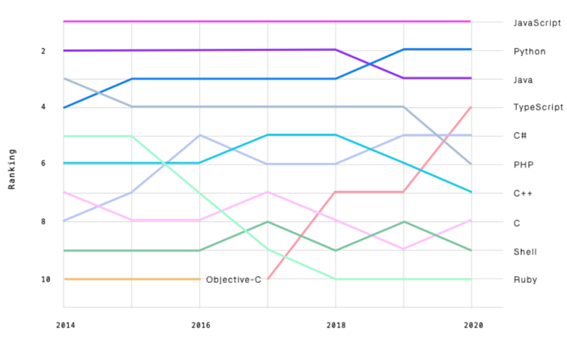
\includegraphics[scale=.75]{github.png}
    \vspace{5pt}
    \legend{Fonte: GitHub stats}
\end{figure}

\subsection{Gitflow}
Gitflow Workflow é um design de fluxo de trabalho Git que foi publicado e popularizado pela primeira vez por Vincent Driessen no nvie. Este define um modelo de ramificação rigoroso, projetado com base no lançamento do projeto, o que oferece uma estrutura robusta para gerenciar projetos maiores. O Gitflow é eficiente para projetos que possuem um ciclo de lançamento agendado, visto que não adiciona novos conceitos ao fluxo de trabalho, mas sim define funções específicas as ramificações e quando devem interagir (SANTACROCE, 2015). Ou seja, em conjunto com o versionamento do GitHub, será mais fácil localizar problemas, caso haja, assim como uma padronização em cada commit é também possível a verificação de o que foi feito de uma forma mais simples e rápida.
\subsection{Vercel}
A Vercel é uma plataforma que hospeda aplicações web front-end de forma gratuita por meio de um CDN\footnote{Central Delivery Network (Rede de Distribuição de Conteúdo) é uma rede de servidores que armazenam réplicas do conteúdo em memória cache do site e as entrega aos usuários visitantes, de acordo com sua localização geográfica de modo que os conecte no servidor mais rápido e mais próximo, fazendo com que se reduza a latência.}
global. Com seus 50 domínios disponíveis e 100Gb de largura de banda, juntamente com sua criptografia SSL fazendo a criptografia necessária dos dados para garantir a segurança. Além disso, há uma integração diretamente com o GitHub, que a cada commit na branch predeterminada é gerado um deploy, que atualizará o site com as últimas alterações. Sua escalabilidade é, segundo sua própria documentação, infinita, sendo que cada camada de sua infraestrutura aumenta e/ou diminui dinamicamente de acordo com o sistema e funções de armazenamento de cache necessários \cite{VERCEL}. 

Internamente na plataforma da Vercel, junto ao o seu framework Next.js, há uma otimização de imagem, que será carregada do servidor de acordo com a área de visualização do dispositivo, guardando-as em cache. Esta otimização reduz o uso de banda, minimizando o tráfego de rede de acordo com o que for necessário para o usuário, melhorando então a experiência geral de quem visita a aplicação.

\subsection{Firebase}
Para o armazenamento das imagens, será utilizado o Firebase Cloud Storage. Este oferece uma forma prática de salvar e recuperar arquivos, incluindo uma das utilizações das imagens, gerando uma url própria para uso. Contendo seu próprio sistema de regras de segurança e acesso como medida protetiva de seus arquivos, permite que apenas clientes autenticados se conectem. Com sua integração diretamente com o JavaScript, apenas a URL no banco de dados será salva, portanto sendo indexada diretamente nos servidores da Google.\cite{FIREBASE}

\subsection{Heroku}
O Heroku é uma plataforma como um serviço, que permite hospedagem, além de configurações e publicações de projetos na nuvem e, diferentemente da Vercel, integra também diversos bancos de dados e possui suporte ao PHP. Com sua integração com o GitHub, seu deploy do projeto é feito a cada commit registrado no sistema, o que facilita a integração. Além disto, esta plataforma é gratuita no seu início contendo uma máquina virtual com 512MB, podendo ser escalável à medida que for necessário com seus custos de infraestrutura. 

Segundo a plataforma é monitorado constantemente por múltiplos servidores a cada dependência, fazendo com que as correções sejam aplicadas assim que possível, tendo uma garantia ao usuário e seus servidores.  Outro detalhe é que a estabilidade em sua plataforma também é garantida por eles, visto que seus algoritmos internos verificam caso ocorra uma queda ou falha na aplicação em tempo de execução e a restaura como uma nova instância automaticamente, garantindo uma preservação dos serviços executados pelo seu usuário sem a necessidade de verificar constantemente o que está ativo \cite{HEROKU}.

\section{Métodos}
Para este projeto, o desenvolvimento será baseado no processo unificado, que propõe etapas as quais são incrementais e interativas, mesmo sendo definido por etapas. Ou seja, tais etapas serão definidas por: concepção, elaboração, construção e transição. Por mais que sejam quatro etapas, como foi dito anteriormente, por mais que sejam as quatro bem definidas, são reexecutadas a cada nova melhoria e funcionalidade da aplicação.

A primeira etapa é dada pela concepção, a qual irá levantar o escopo do projeto de forma mais genérica, sendo o caso de uso, que será incrementado a cada nova funcionalidade. Este por sua vez, irá demonstrar como será a interação dos usuários, chamados de atores, com o sistema e suas funcionalidades, que são os casos de uso para cada um. Sendo assim, os atores identificados inicialmente são: supervisor, associado, usuário, visitante e o apresentador, podendo serem vistos no caso de uso representado pela figura \ref{fig_caso_uso}.

\begin{figure}[H]
    \caption{\label{fig_caso_uso}Caso de uso}
    \vspace{5pt}
    \centering
    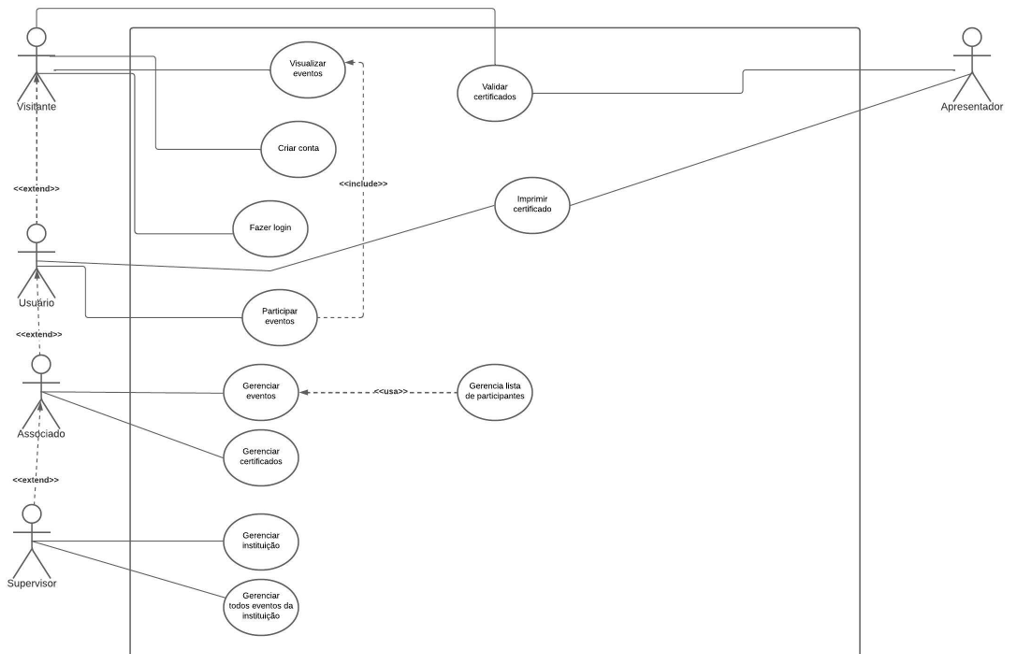
\includegraphics[scale=.4]{caso de uso.png}
    \vspace{5pt}
    \legend{Fonte: Próprio autor}
\end{figure}

Há cinco níveis de acesso ao sistema, sendo estes:
\begin{itemize}
    \item \textbf{Visitante: } não possui cadastro no sistema ou não entrou em sua conta ainda, portanto seu processo estará pré-definido de forma que possa visualizar os eventos, mas não poderá participar destes. Além disso, poderá criar conta e fazer login, no que se diz a respeito do seu cadastro e por fim poderá validar os certificados de terceiros, caso tenha a chave necessária.
    \item \textbf{Usuário: interage com o sistema de modo que poderá gerenciar seu perfil, fazendo alterações em áreas determinadas de seu cadastro. Além disso, poderá participar de eventos, os quais irão gerar certificados que poderão ser convertidos para arquivos e salvos no computador, além de serem enviados por email caso tenham participado do evento. Vale ressaltar que estas ações só poderão ser feitas após a realização do login. E para que seja feito isto, é necessário que seja feito um cadastro na aplicação utilizando-se de dados pessoais tais como: nome completo, email, CPF e telefone para que sejam gerados os certificados de forma correta. }
    \item \textbf{Apresentador: tem como principal função, podendo ou não ter um cadastro na aplicação, ser vinculado a um evento o qual irá apresentar. Ou seja, supondo que seja uma palestra, este será o palestrante e terá acesso ao seu certificado por meio do email cadastrado no evento. Caso já tenha um cadastro, este será vinculado diretamente a conta e poderá ser impresso (sem a necessidade de consulta ao email) diretamente da aplicação.}
    \item \textbf{Associado: tem acesso a tudo que um usuário faz, mas poderá gerir até certo nível a instituição, fazendo a criação de eventos acadêmicos. Para que alguém se torne associado, é necessário que o supervisor o vincule a uma instituição. Sua principal função é gerir os eventos criados pelo próprio autor, de forma que serão vinculados a este por meio da instituição.}
    \item \textbf{Supervisor: tem a função de criar e gerir a instituição, além de gerir todos os eventos pertencentes a esta.}
\end{itemize}


\subsection{API}
A API para a aplicação será feita em Laravel com utilização do SGBD MySQL por meio de uma autenticação segura. As consultas e requisições ao banco de dados serão feitas nesta camada. E seu retorno dos dados requisitados serão transmitidos ao módulo de visão via JSON.

Além disso, a autenticação da aplicação será validada por meio do JWT\footnote{JSON Web Token (JWT) é um padrão aberto (RFC 7519) que define uma maneira compacta e independente para transmitir informações com segurança entre as partes como um objeto JSON. Essas informações podem ser verificadas e confiáveis porque estão assinadas digitalmente.} a autenticidade do usuário, ou seja, para cada requisição que exija segurança, como por exemplo a criação de um evento ou alterações na conta do usuário, que dizendo de forma geral, qualquer alteração solicitada ao SGBD. Isto garantirá que o usuário está devidamente conectado, assim como que sua autenticidade.

\subsection{Front-end}
O front-end será feito em Next.js, na qual irá receber os dados referentes a API e convertê-los para uma interface ao usuário. Esta interface será um site no qual, usuário poderá interagir e fazer todas as ações permitidas. Além disso, este módulo feita de forma que seja simples, fácil empregando conceitos de usabilidade para uma melhor experiência.\\
Para evitar fraudes com bots, será necessário utilizar um sistema que verifique isto, principalmente na criação de usuários, assim como no login destes que é onde vem a ideia do CAPTCHA\footnote{O CAPTCHA (Teste de Turing público completamente automatizado para distinguir entre computadores e pessoas) é um tipo de medida de segurança conhecido como autenticação por desafio e resposta. O CAPTCHA protege contra spam e descriptografia de senhas com um teste simples que prova que você é um ser humano, não um computador tentando invadir uma conta protegida por senha.}. A implementação utilizada foi o hCaptcha\footnote{O hCAPTCHA é um serviço de CAPTCHA gratuito e independente que fornece desafios fáceis para humanos, entretanto são complexos para uma máquina, tais como classificação de um objeto dada as imagens.}, o qual irá proteger o sistema de login da aplicação, dificultando o acesso para máquinas automatizadas.

\subsection{Versionamento}
O versionamento será feito utilizando o Git, por meio de um repositório no Github. Cada versão será feita com base nos critérios do GitFlow, seguindo a lógica descrita de master e develop, sendo a primeira a versão de produção e a outra sendo a versão com as novas funcionalidades e para testes. Cada parte da aplicação terá seu versionamento de acordo com sua funcionabilidade, ou seja, a API terá seu versionamento separado do front-end.

%\begin{lstlisting}[caption={A simple caption}]
 %x := -2 + y
 %\end{lstlisting}

% -----------------------------------------
\chapter{Projeto e Desenvolvimento}\label{chp:LABEL_CHP_4}
% -----------------------------------------
Nesta seção são detalhados os passos e decisões tomadas ao decorrer do período de desenvolvimento deste trabalho. São apresentadas as etapas de implementação e integração com outras soluções utilizadas, assim como a execução e comparação dos resultados obtidos.

\section{Casos de uso}
Inicialmente foi desenvolvido o caso de uso expandido do sistema, baseando-se no que foi demonstrado por \citeonline{SOMMERVILE} do modelo UML, como forma tanto de documentação, assim como planejamento do protótipo. Todas as interações do sistema com seus usuários foram pré-determinadas, assim como a definição e organização de requisitos funcionais no sistema dado seu contexto para modelagem do fluxo básico dos eventos diretamente nestes diagramas. O caso de uso, mostra neste contexto o escopo da aplicação, trazendo as principais funcionalidades em que foram desenvolvidas no protótipo, limitando-se a eventos educacionais online. Os cenários de interação entre os atores por meio do caso de uso determinado definem principalmente como deveria ser planejado e até qual ponto pode ser utilizado por cada um deles, respeitando sua hierarquia. A figura \ref{caso_uso_1} demonstra o primeiro caso de uso planejado para o protótipo.

\begin{figure}[H]
    \caption{\label{caso_uso_1}Primeiro caso de uso}
    \vspace{5pt}
    \centering
    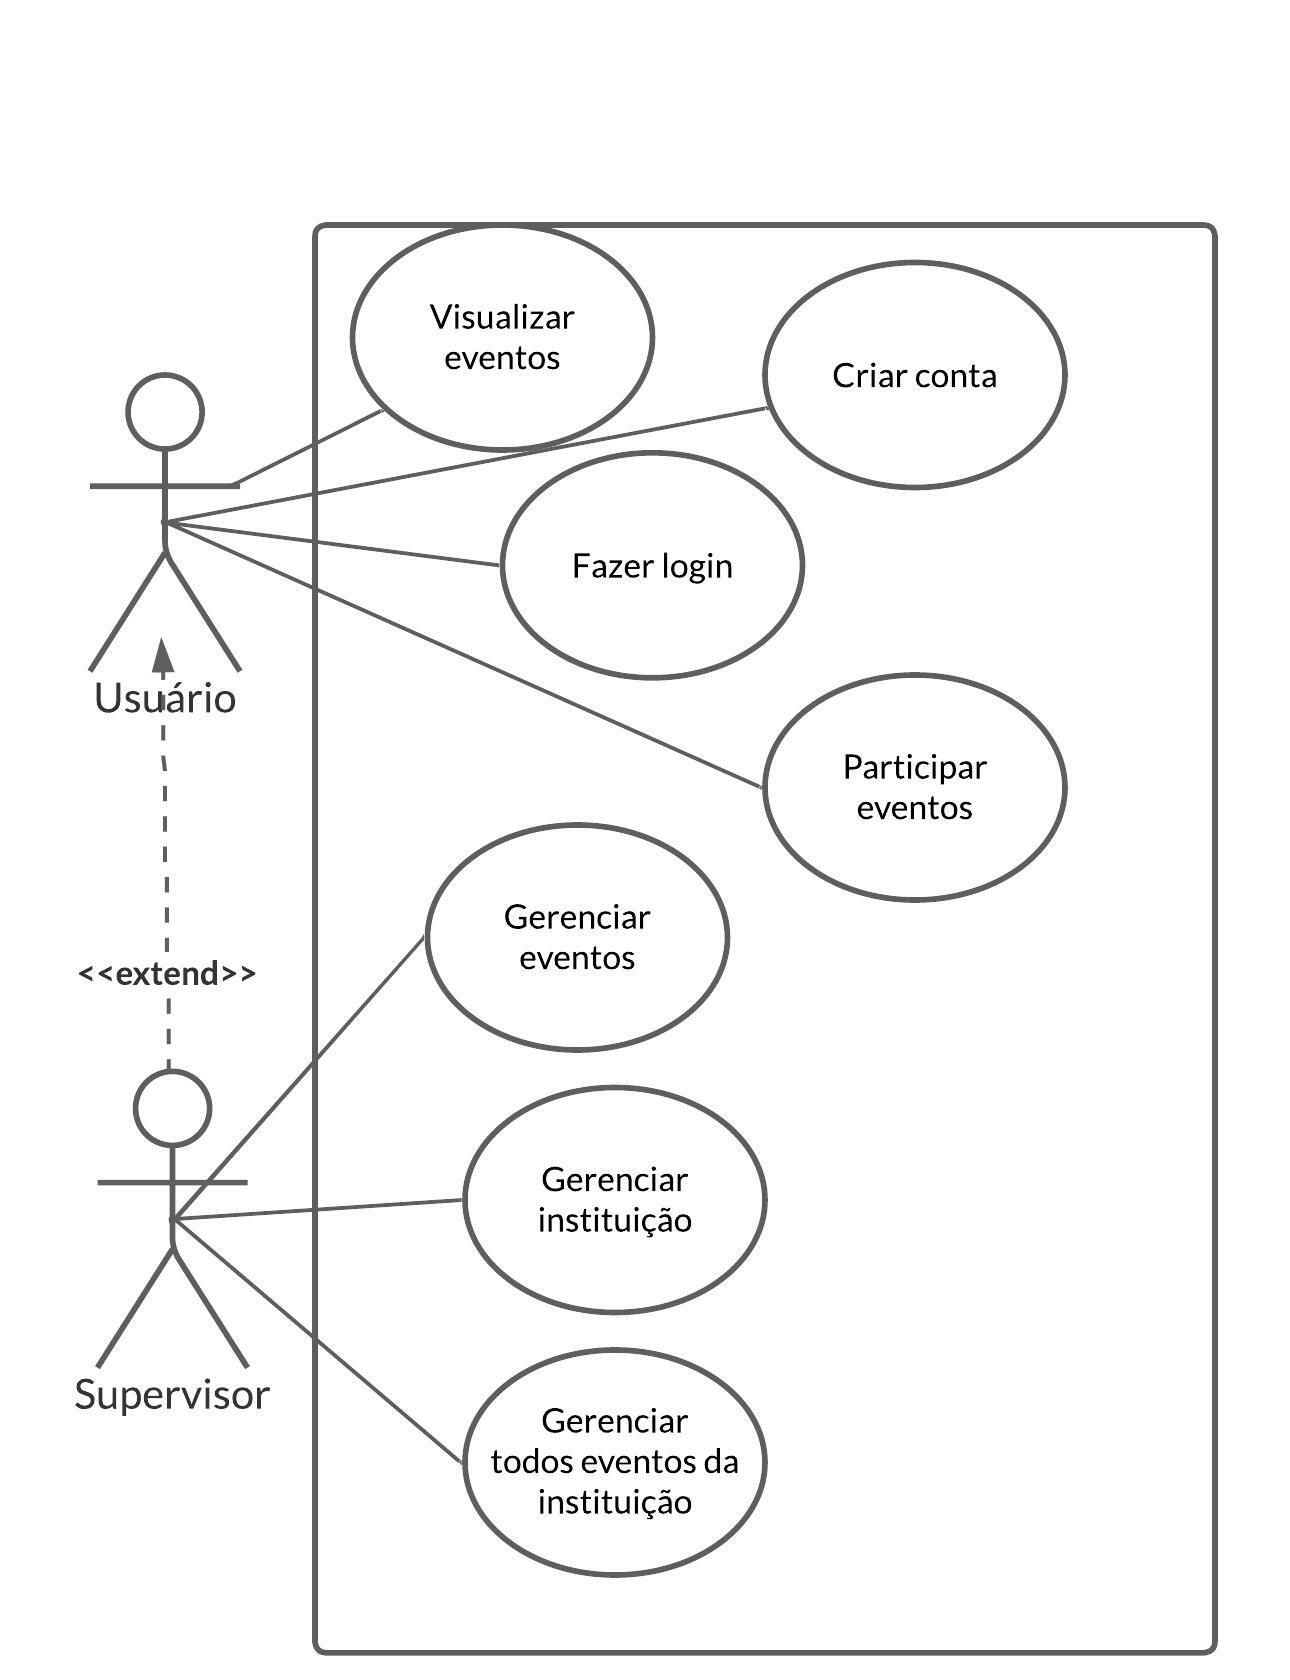
\includegraphics[scale=.6]{Caso de uso TCC1.jpeg}
    \vspace{5pt}
    \legend{Fonte: Próprio autor}
\end{figure}


Com base nesse diagrama, e sua devida explicação, foi possível traçar uma rota de desenvolvimento por meio do processo unificado. No início foi pensado em apenas dois atores, sendo estes um administrador e um usuário comum, como mostra a imagem. Nisto, foram desenvolvidas funcionalidades básicas para estes, contendo a primeira iteração, sem os demais. 

Para a segunda iteração, já há mais atores contando com a inclusão do associado, sendo intermediário entre usuário e supervisor. Além disso, e novas funcionalidades pensadas para a aplicação, sendo estas a gerência da lista de participantes e a gerência dos eventos apenas para determinado usuários (sendo estas relacionadas ao associado) conforme demonstrado na figura \ref{caso_uso_2}.

\begin{figure}[H]
    \caption{\label{caso_uso_2}Segundo caso de uso}
    \vspace{5pt}
    \centering
    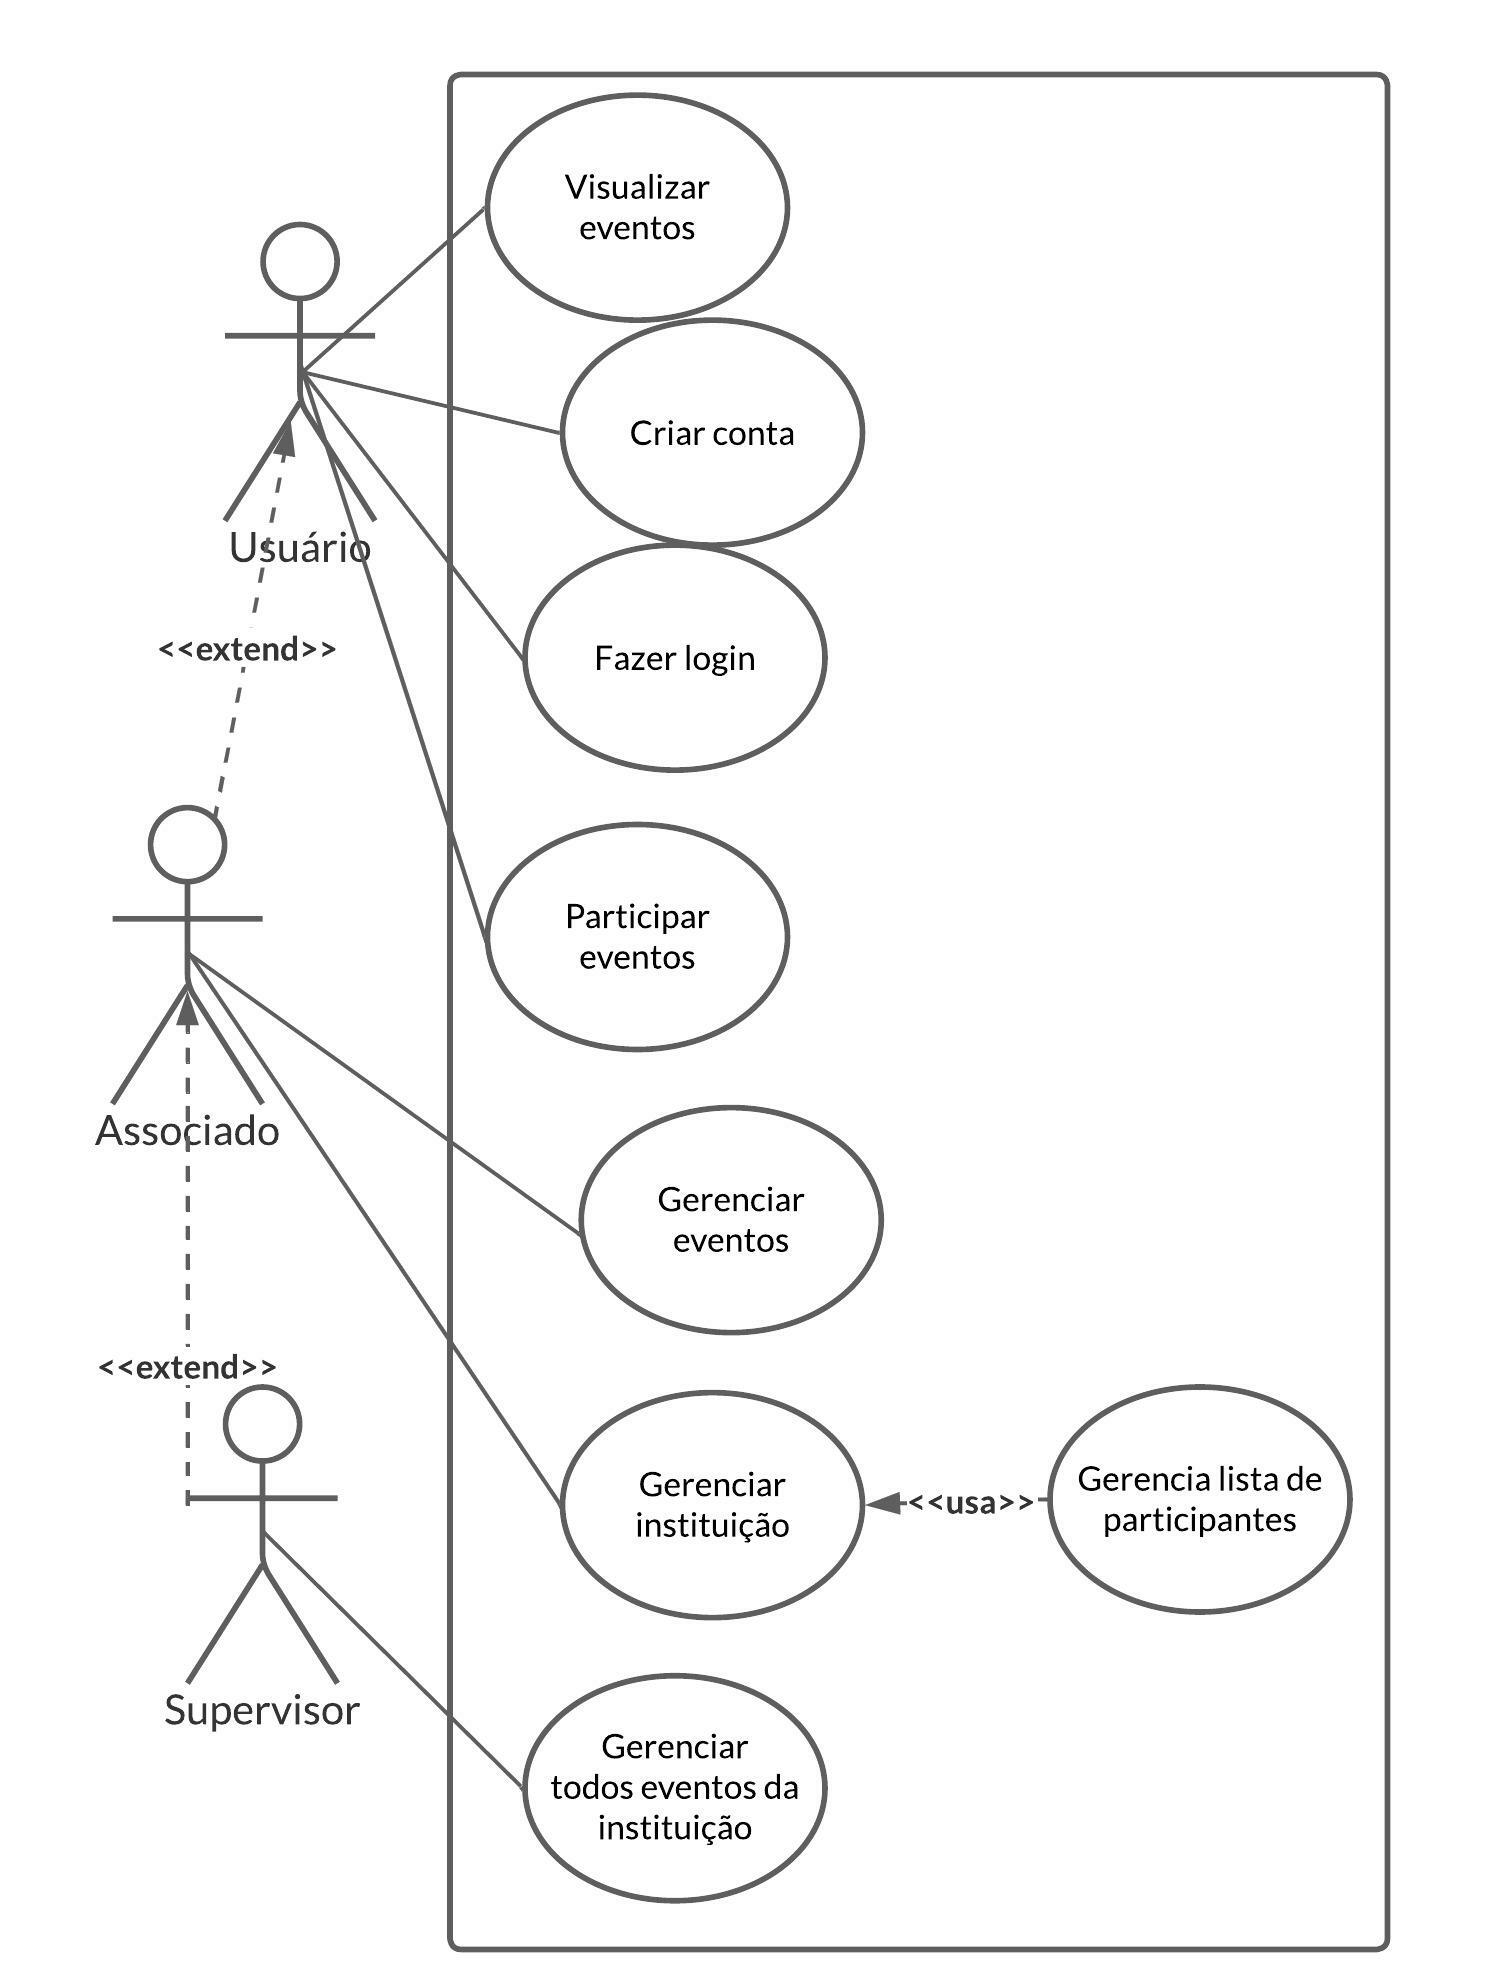
\includegraphics[scale=.7]{Caso de uso TCC2.jpeg}
    \vspace{5pt}
    \legend{Fonte: Próprio autor}
\end{figure}

Na terceira iteração foram identificadas necessidades de atores que não precisavam necessariamente de um \textit{login}, como o visitante, que poderá apenas visualizar os eventos e validar certificados, operações mais simples e que não necessitam de qualquer permissão especial conforme o que é exibido na figura \ref{caso_uso_3}. 

\begin{figure}[H]
    \caption{\label{caso_uso_3}Terceiro caso de uso}
    \vspace{5pt}
    \centering
    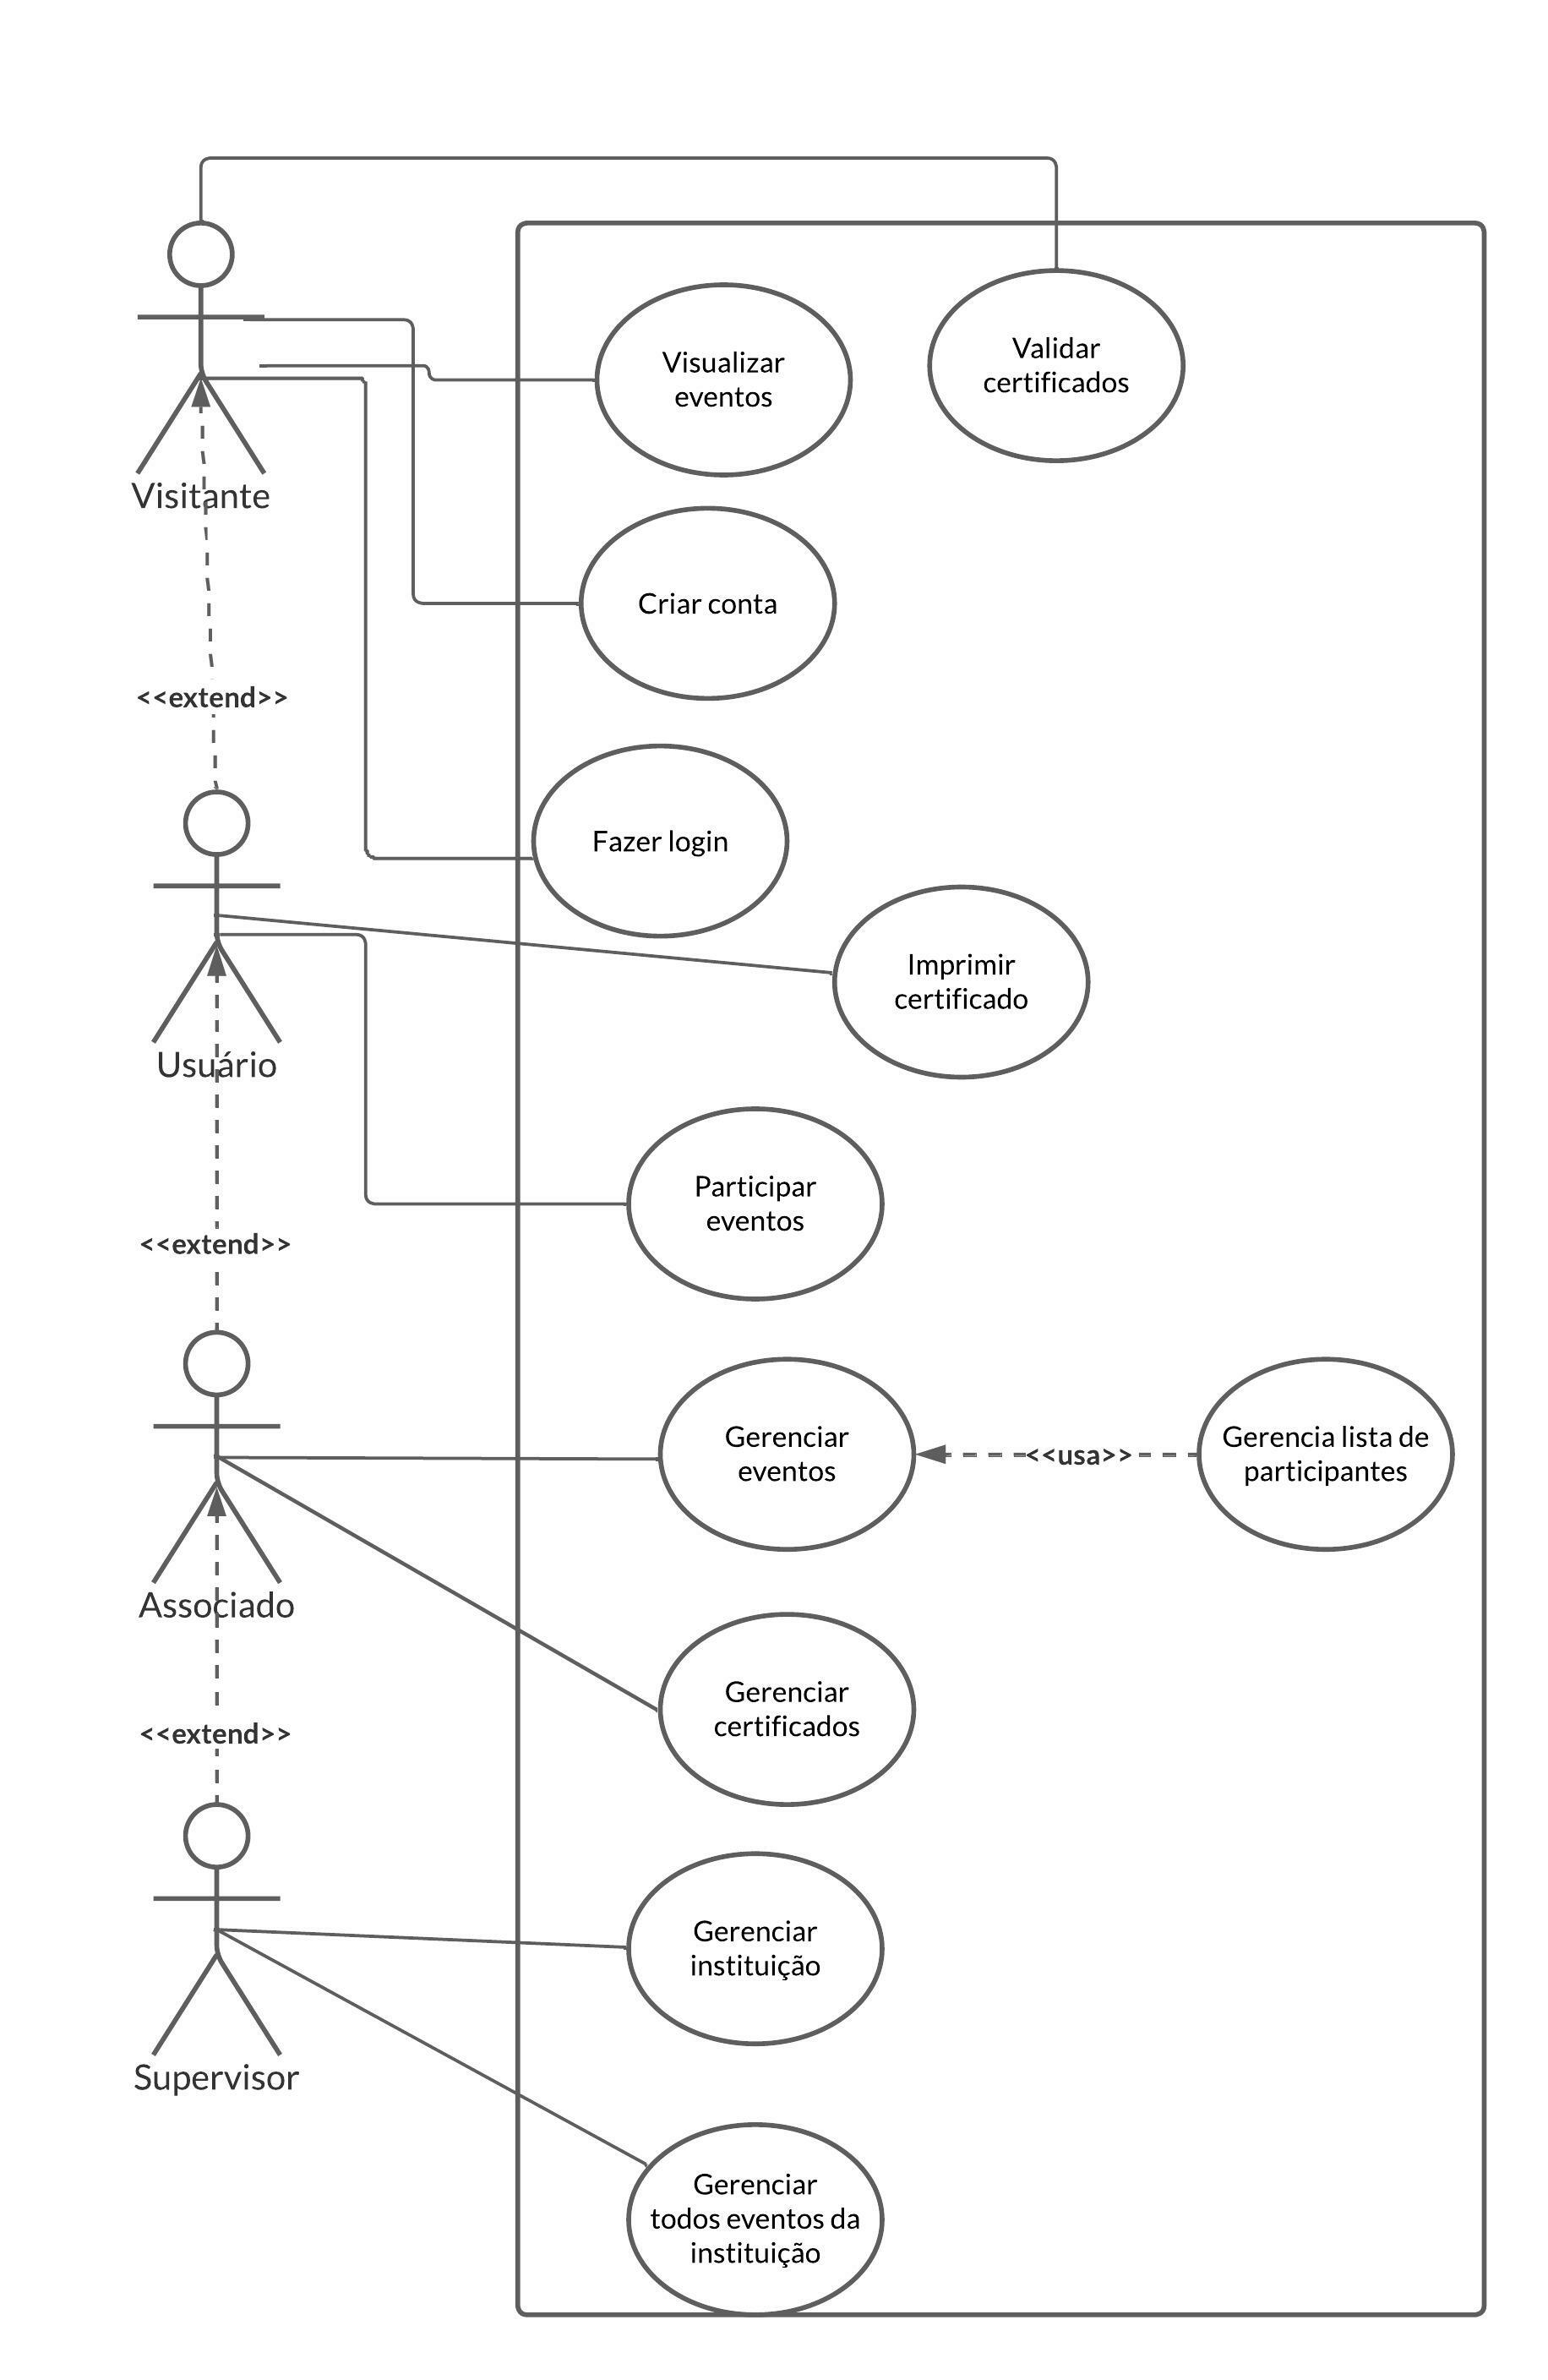
\includegraphics[scale=.7]{Caso de uso TCC3.jpeg}
    \vspace{5pt}
    \legend{Fonte: Próprio autor}
\end{figure}

Na quarta e última iteração até o momento o sistema está mais moldado pensando em diversas funcionalidades, inclusive com o caso de uso expandido, tendo em vista melhor as funcionalidades e seus retornos do sistema para o ator determinado conforme a figura \ref{caso_uso_4}.

\begin{figure}[H]
    \caption{\label{caso_uso_4}Quarto caso de uso}
    \vspace{5pt}
    \centering
    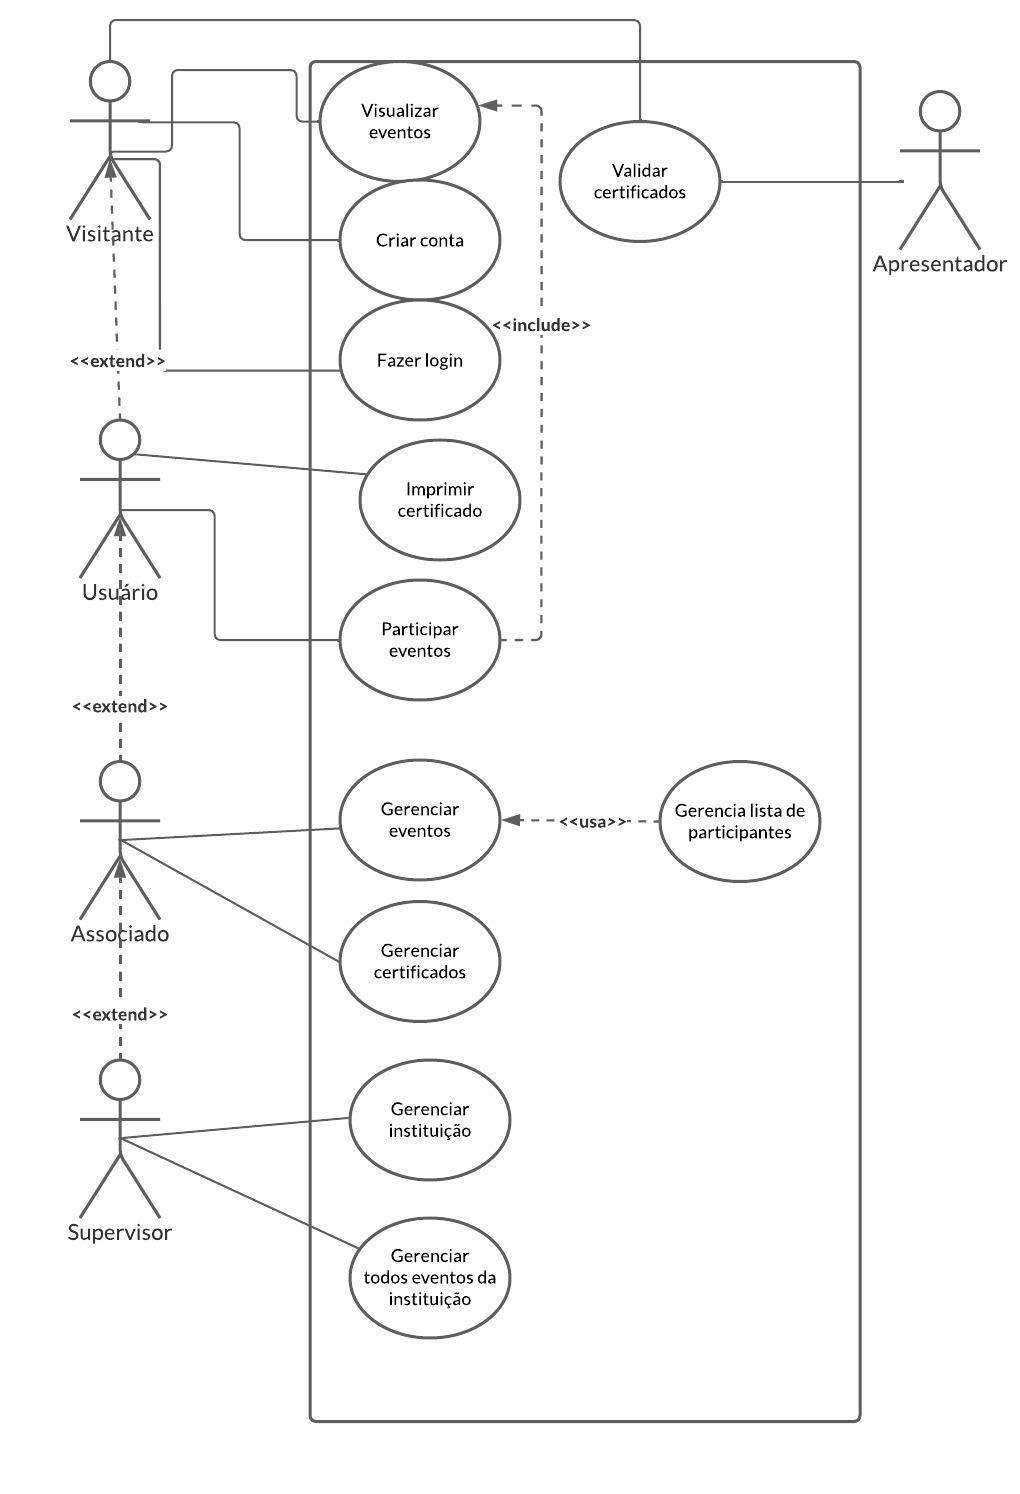
\includegraphics[scale=.7]{Caso de uso TCC4.jpeg}
    \vspace{5pt}
    \legend{Fonte: Próprio autor}
\end{figure}

\subsection{Caso de uso expandido}
Segundo \citeonline{WAZLAWICK}, o caso de uso expandido corresponde ao aprofundamento da análise de requisitos, ou seja, descreve-se mais detalhadamente os passos para cada caso de uso documentado, conforme demonstrado abaixo:

\begin{itemize}
    \item CSU01: visualizar eventos 
        \begin{itemize}
            % \item Pré-condições:
            \item Descrição: O sistema apresenta uma lista de eventos e o usuário pode selecionar um evento para visualização mais detalhada.
            % \item Pós-condições
        \end{itemize}
    \item CSU02: Criar conta
    \begin{itemize}
            \item Descrição: O usuário informa o nome, e-mail, telefone, CPF e senha. O sistema valida as informações digitadas e cria a conta.
            \item Pós-condições: Um e-mail é enviado ao usuário para verificação.
        \end{itemize}
    \item CSU03: Fazer login
        \begin{itemize}
            \item Pré-condições: O usuário deve ter criado a conta anteriormente com o e-mail validado.
            \item Descrição: O usuário informa o e-mail e senha. O sistema valida as informações digitadas e realiza o login.
            \item Pós-condições: O sistema deixa salvo as informações para que, na próxima entrada do usuário, não seja necessário digitar novamente os dados.
            \end{itemize}
    \item CSU04: Imprimir certificado
        \begin{itemize}
            \item Pré-condições: O usuário deve ter participado anteriormente de um evento.
            \item Descrição: O participante ou apresentador geram o arquivo PDF do evento selecionado.
        \end{itemize}
    \item CSU05: Participar eventos
        \begin{itemize}
            \item Pré-condições: O usuário deve ter efetuado o login e selecionado um evento previamente.
            \item Descrição: O participante seleciona as atividades de um determinado evento e participa destas.
            \item Pós-condições: O associado ou supervisor podem selecionar quem foi ao evento para geração do certificado.
        \end{itemize}
    \item CSU06: Gerenciar eventos
        \begin{itemize}
            \item Pré-condições: O usuário deve ter feito login com permissão de associado ou supervisor e selecionar um evento que ainda não ocorreu nenhuma de suas atividades.
            \item Descrição: O usuário pode editar, excluir eventos já cadastrados no sistema. Na edição será possível alterar atividades, descrição e apresentadores.
        \end{itemize}
    \item CSU07: Gerenciar certificados
        \begin{itemize}
            \item Pré-condições: O usuário deve ter efetuado login com permissão de associado ou supervisor.
            \item Descrição: O usuário pode criar, editar ou excluir modelos padrões de certificado. Para criação é necessário que informe a imagem de fundo, banner e assinatura, um título e nome e cargo de quem irá assinar.
            \item Pós-condições: o sistema irá gravar as informações e poderão ser utilizadas para qualquer certificado de evento.
        \end{itemize}
    \item CSU08: Gerenciar instituição
        \begin{itemize}
            \item Pré-condições: O usuário deve ter efetuado login com permissão de supervisor.
            \item Descrição: É possível alterar dados da instituição como seu nome, o supervisor e gerenciar os associados. Ao alterar o supervisor ou adicionar um associado, o sistema verifica se é um usuário válido.
        \end{itemize}
    \item CSU09: Gerenciar todos os eventos da instituição
        \begin{itemize}
            \item Pré-condições: O usuário deve ter efetuado login com permissão de supervisor.
            \item Descrição: O supervisor pode alterar qualquer evento da instituição, sendo ou não criado por seu usuário.
        \end{itemize}
    \item CSU10: Validar certificados
        \begin{itemize}
            \item Descrição: O usuário informa o código de verificação do certificado.
            \item Pós-condições: O sistema retorna se o certificado é válido ou não.
        \end{itemize}
    \item CSU11: Gerencia lista de participantes
        \begin{itemize}
            \item Pré-condições: O usuário deve ter efetuado login com permissão de supervisor ou associado e selecionado um evento.
            \item Descrição: O usuário pode selecionar quem participou do evento, seja participante ou apresentador para gerar um certificado.
            \item Pós-condições: O certificado em formato PDF é enviado ao e-mail dos participantes e apresentadores selecionados.
        \end{itemize}
        
\end{itemize}

\section{Mockups}
Dados os casos de uso, será possível criar um mockup das telas baseado nestas informações. Ou seja, a criação de telas por meio do Figma possibilitou a visualização e alteração do layout de uma forma simplificada antes de serem implementadas de fato. Dito isso, toda o mockup foi pensado para seguir padrões na interface, como, por exemplo, a barra de navegação está presente em todas as páginas a qual o usuário poderá navegar (com exceções apenas da criação de conta e login). E isto facilita a navegação, e mantém a similaridade da aplicação para o usuário final.  

A figura \ref{home_mockup} demonstra como é a ideia da página inicial, que contém uma barra de navegação, um acesso aos eventos, um acesso à criação de eventos e ao perfil. Haverá, no meio da página, um destaque aos últimos eventos cadastrados na plataforma, podendo ser acessados diretamente desta página.
\begin{figure}[H]
    \caption{\label{home_mockup}Mockup da tela inicial}
    \vspace{5pt}
    \centering
    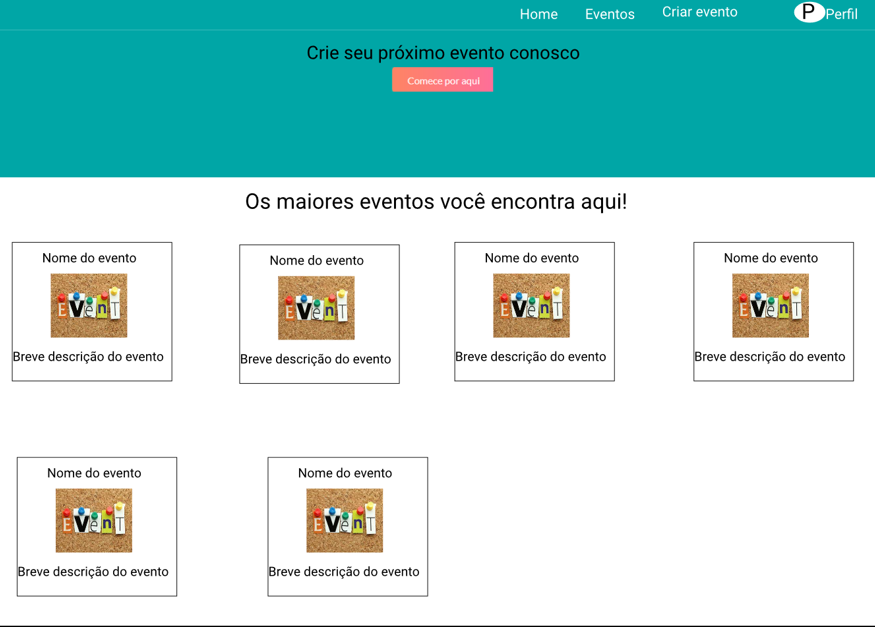
\includegraphics[scale=.4]{home_mockup.png}
    \vspace{5pt}
    \legend{Fonte: Próprio autor}
\end{figure}

Para a página seguinte, a figura \ref{evento_mockup} mostra como é a visualização detalhada de um evento, com sua descrição, imagem e suas atividades cadastradas. Estes detalhes são os compostos especificamente para um evento, mas a barra de navegação citada anteriormente na página inicial estará presente para facilitar a navegação entre páginas.
\begin{figure}[h]
    \caption{\label{evento_mockup}Mockup da tela do evento}
    \vspace{5pt}
    \centering
    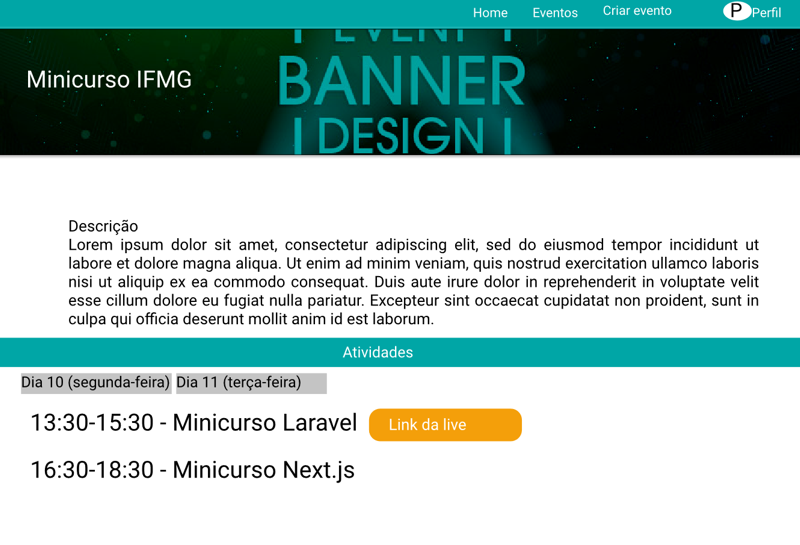
\includegraphics[scale=.4]{evento_mockup.png}
    \vspace{5pt}
    \legend{Fonte: Próprio autor}
\end{figure}

A terceira parte do mockup é a tela de pesquisa de eventos, como mostra a figura \ref{pesquisa_mockup}, que assim como as demais mantém a barra de navegação para facilitar o acesso e possui diversos filtros para os eventos. Estes filtros, definidos por categoria, instituição, data inicial e final e horário inicial e final, foram definidos como os principais para a pesquisa. E ao final da página, percebe-se a paginação, ou seja, caso passe de uma determinada quantidade, serão criadas diversas abas possíveis da mesma pesquisa.
\begin{figure}[H]
    \caption{\label{pesquisa_mockup}Mockup da tela de pesquisa}
    \vspace{5pt}
    \centering
    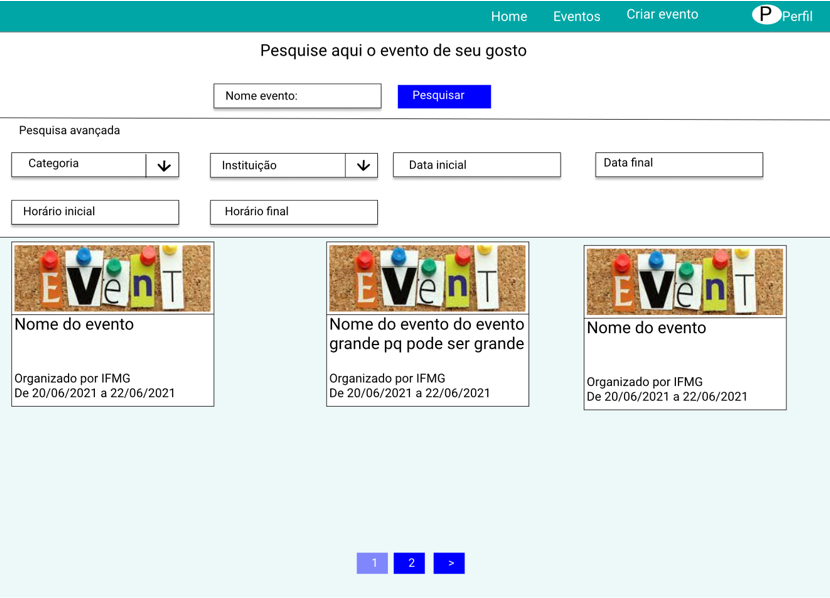
\includegraphics[scale=.4]{pesquisa_mockup.png}
    \vspace{5pt}
    \legend{Fonte: Próprio autor}
\end{figure}

Por fim, a figura \ref{form_mockup}, mostra como serão todos os formulários do sistema, sendo este utilizado conforme a necessidade da tela, como a criação de eventos ou criação de usuário. Isto se deve para melhorar tal interação, tornando padronizado e fazendo com que não seja necessário retrabalho de aprendizagem para cada página contida.
\begin{figure}[H]
    \caption{\label{form_mockup}Mockup da tela de formulário padrão}
    \vspace{5pt}
    \centering
    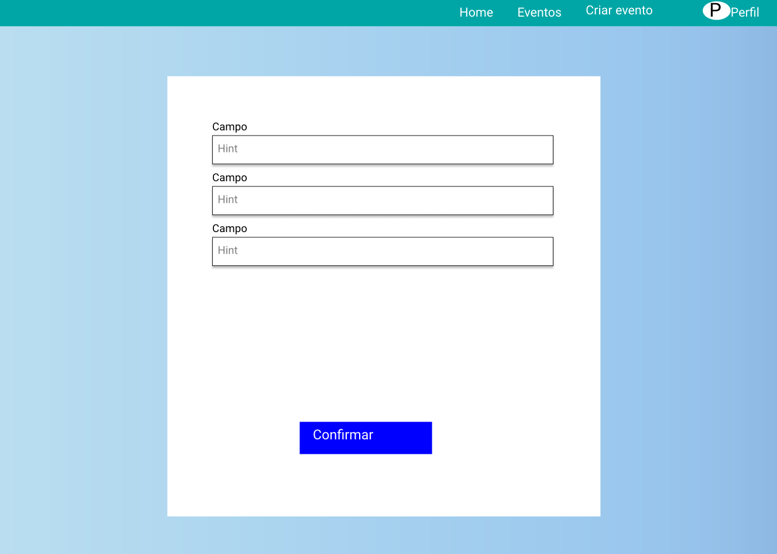
\includegraphics[scale=.4]{form_mockup.png}
    \vspace{5pt}
    \legend{Fonte: Próprio autor}
\end{figure}

Com estas informações sobre a responsabilidade e design de cada tela da aplicação, é possível a criação de maneira estruturada, além de padronizada da interface para o usuário. 

\section{Estruturação}
A estruturação segue um modelo de distribuição vertical, o qual prevê a distinção entre divisão de componentes, neste caso a interface com o usuário e a API, em dois servidores distintos, sendo um alocado na Vercel e outro no Heroku. Mesmo que uma aplicação dependa da outra para funcionar integralmente, são serviços distintos e que melhoram de maneira geral o funcionamento do sistema, visto que tais responsabilidades distintas melhoram o tempo de carregamento de acordo com \citeonline{COULOURIS}. Ou seja, enquanto \textit{backend} persiste os dados e os processa diretamente, respondendo a requisições, o \textit{frontend} fará as requisições recuperando o arquivo JSON gerado e o transformando em uma interface gráfica tangível ao usuário.


\section{Modelo de banco de dados}
Nesta etapa foram criados modelos os quais tiveram embasamento no diagrama de Caso de Uso, assim como nos mockups, visto que deve atender os requisitos predeterminados. Foram criados os modelos conforme figura \ref{modelo_banco}, que determina cada classe do banco de dados feita no Laravel para poder representar os relacionamentos entre as tabelas do MySQL, além de determinar cada atributo das classes. Estes foram feitos com base na figura \ref{models_projeto}, que representa o diagrama de entidade e relacionamento do banco de dados.
\begin{figure}[H]
    \caption{\label{models_projeto}Classes de modelo}
    \vspace{5pt}
    \centering
    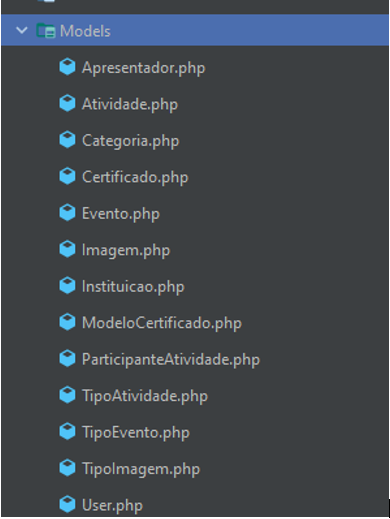
\includegraphics[scale=.8]{models_projeto.png}
    \vspace{5pt}
    \legend{Fonte: Próprio autor}
\end{figure}
\begin{figure}[htbp]
    \caption{\label{modelo_banco}DER do banco de dados}
    \vspace{5pt}
    \centering
    % \includesvg[inkscapelatex=false, width = 100pt]{modelo.svg}
    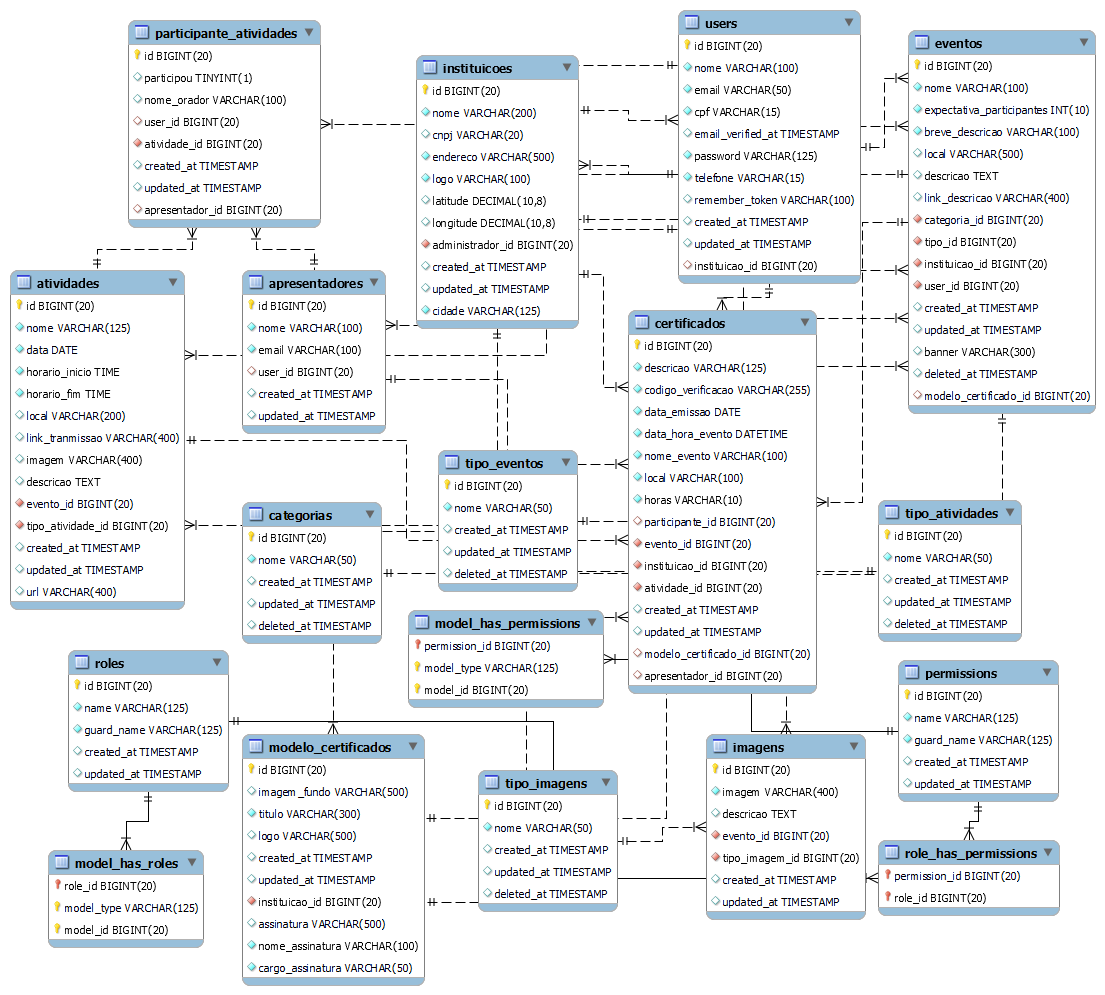
\includegraphics[scale=.5, angle = -90]{modelo.png}
    \vspace{5pt}
    \legend{Fonte: Próprio autor}
\end{figure}
O banco de dados foi planejado criando-se a partir das funcionalidades da aplicação. As tabelas são descritas abaixo:
\begin{itemize}
    \item \textbf{\textit{Users}:} tabela de usuários, com informações básicas do cadastro, contendo nome, e-mail, CPF, senha e telefone. O campo senha é criptografado de modo que tenha segurança ao gravar os dados. Os campos e-mail e CPF devem ser únicos no banco. E há um campo de chave estrangeira, relacionado a instituição, podendo ser nulo, que caso o usuário esteja vinculado a uma instituição, será atribuído o id a ele.
    
    \item \textbf{Instituicoes:} tabela que contém as informações referentes as instituições, tais como o nome, CNPJ, endereço e cidade. O campo CNPJ deve ser único. A chave estrangeira administrador\_id é relacionada ao usuário que criou ou foi transferida a administração da instituição.
    
    \item \textbf{Categorias:} tabela criada com intuito de categorizar os eventos de modo que seja facilitada a busca na aplicação.
    
    \item \textbf{Tipo\_Eventos:} tabela criada com intuito de sub-categorizar os eventos de modo que seja facilitada a busca na aplicação
    
    \item \textbf{Tipo\_Atividades:} tabela criada com intuito de categorizar as atividades de modo que seja facilitada a busca na aplicação.
    
    \item \textbf{Eventos:} tabela que possui os dados do evento, como seu título, expectativa de participantes, banner e uma breve descrição como obrigatórios. Os campos opcionais, como local, descrição podem ser adicionados depois, não sendo obrigatórios. O campo banner é uma URL da imagem armazenada no Firebase. As chaves estrangeiras são definidas pela categoria\_id, tipo\_id (ambas referentes às categorias e tipos escolhidos pelo usuário), instituicao\_id e user\_id (ambas referentes ao usuário que criou o evento) e chave modelo\_certificado\_id (não obrigatória para criação do evento, mas obrigatória para criação dos certificados posteriormente).
    
    \item \textbf{Modelo\_Certificados:} a tabela para os modelos de certificado deve conter os campos de título, nome\_assinatura e cargo\_assinatura como obrigatórios, sendo textos. Os campos de imagem\_fundo, assinatura e logo devem ser preenchidos com as URLs das imagens armazenadas no Firebase. A chave estrangeira instituicao\_id se refere a instituição que criou tal modelo.
    
    \item \textbf{Apresentadores:} os apresentadores podem ser externos à aplicação, então contêm um nome e e-mail. Caso o e-mail seja vinculado a um usuário, será atribuído um id de usuário nesta tabela.
    
    \item \textbf{Tipo\_Imagens:} descreve o tipo de imagem que está no evento, podendo ser banner ou outros.
    
    \item \textbf{Imagens:} tabela que armazena a URL da imagem contida no Firebase, com as chaves estrangeiras de seu tipo e do evento que foi vinculada.
    
    \item \textbf{Atividades:} as atividades são descritas pelo seu nome, a data que irá ocorrer, assim como horário de início e término como obrigatório. Descrição e local podem ser inseridos posteriormente. A URL também pode ser inserida posteriormente, mas é necessário que tenha a URL para que a atividade ocorre, sendo que é com base nela que os participantes entraram. As chaves estrangeiras são: evento\_id, referenciando o evento da atividade e a tipo\_atividade\_id que é sobre o tipo de atividade selecionado.
    
    \item \textbf{Certificados:} esta tabela descreve todas as informações presentes do evento, atividade, data, e as horas da atividade. Deve conter um modelo de certificado para poder se basear as informações. O certificado pode ser para um participante, que deve ser usuário da aplicação, ou um apresentador, podendo este ser externo a aplicação.
    
\end{itemize}

\section{Controllers}
Por meio dos controladores do Laravel, é possível manipular as operações do banco de dados, e para haver uma organização e mantenha o padrão MVC, foram criados controladores específicos para cada modelo, sendo cada um atribuído a responsabilidade do modelo correspondente e essa estruturação pode ser vista na figura \ref{controllers}, a qual demonstra cada um dos controladores.
\begin{figure}[H]
    \caption{\label{controllers}Controladores}
    \vspace{5pt}
    \centering
    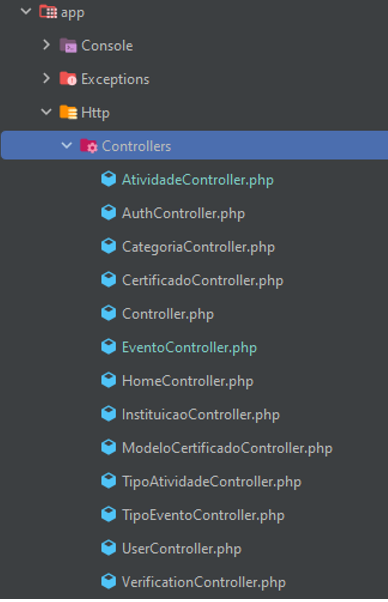
\includegraphics[scale=.5]{controllers.png}
    \vspace{5pt}
    \legend{Fonte: Próprio autor}
\end{figure}

Além disso, por fazerem parte de uma API (explicada com mais detalhes posteriormente), cada operação deve retornar um JSON, com o código de status de retorno do HTTP. No trecho de código, visto no código \ref{orm}, é um exemplo da função a qual recebe uma requisição determinando cada um dos filtros, e então por meio do \textit{eloquent ORM}, realizando a \textit{query} no banco de dados e no fim retornando um JSON com os dados, padronizando, então, a maneira de se receber e retornar os dados.
\begin{lstlisting}[language=PHP, caption = {Exemplo do ORM} \label{orm}]
 public function index(Request $request): JsonResponse {
        $eventos = Evento::query()->with(['atividades' => function ($query) {
            $query->orderBy('data')
            ->orderBy('horario_inicio')
            ->orderBy('horario_fim')
            ->orderBy("nome");
        }, 'categoria', 'instituicao'])
            ->whereHas('atividades')
            ->orderBy('created_at', 'desc');

        if ($request->titulo != null) {
            $queryLower = trim(strtolower($request->titulo));
            $eventos->where(function ($query) use ($queryLower) {
                $query->where(DB::raw('lower(nome)'), 'like', '%' . $queryLower . '%')
                    ->orWhere(DB::raw('lower(breve_descricao)'), 'like', '%' . $queryLower . '%');
            });
        }

        if ($request->cat != null) {
            $eventos->whereRelation('categoria', 'categorias.id', '=', $request->cat);
        }

        if ($request->instituicao != null) {
            $eventos->whereRelation('instituicao', 'instituicoes.id', $request->instituicao);
        }

        if ($request->dataInicio != null) {
            if ($request->dataFim != null) {
                $eventos->whereHas('atividades', function ($q) use ($request) {
                    $q->whereBetween('data', [$request->dataInicio, $request->dataFim]);
                });
            } else {
                $eventos->whereRelation('atividades', 'atividades.data', $request->dataInicio);
            }
        }

        if ($request->horarioInicio != null) {
            $eventos->whereHas('atividades', function ($q) use ($request) {
                $q->whereTime('atividades.horario_inicio', '>=', $request->horarioInicio);
            });
        }

        if ($request->horarioFim != null) {
            $eventos->whereHas('atividades', function ($q) use ($request) {
                $q->whereTime('atividades.horario_fim', '<=', $request->horarioFim);
            });
        }

        return response()->json($eventos->paginate(20));
    }
\end{lstlisting}

Dado o exemplo da busca e seus filtros, a validação de dados na inserção e atualização de dados é essencial para não haver dados inseridos de maneira indevida e que haja um padrão nas requisições. Isto tudo é feito diretamente no Laravel, que validará antes mesmo do banco de dados e retornará caso haja algum erro.

\section{Operações API}
A API foi feita no Laravel, respeitando os padrões estabelecidos pela interface REST. Ou seja, por meio de requisições HTTP do tipo GET, POST e DELETE é possível acessar todas as rotas do \textit{backend}. Em diversas destas não será possível acessar sem que haja uma autenticação feita por meio do JWT, que irá validar se há permissão de acesso, e isto determina caso o usuário esteja logado, assim como seu nível de acesso dentro de sua hierarquia. 

As rotas foram criadas em grupos para atenderem as necessidades e criar-se uma organização para cada requisição, então foram organizadas, conforme o código \ref{rotas_laravel}. Este demonstra cada um dos agrupamentos, sendo estes aqueles que contém todas as rotas para modelos, assim como para determinadas funcionalidades do sistema. O grupo de eventos tem todas as rotas pertencentes a eventos  e conforme pode ser visualizado possuem autenticação e validação do que pode ser escrito na URL para poder ser acessada devidamente. 

\begin{lstlisting}[language=PHP, caption = {Grupo de rotas} \label{rotas_laravel}]
 Route::group(["prefix" => "eventos"], function () {
    Route::get("/", [EventoController::class, 'index']);
    Route::get("/{id}", [EventoController::class, 'show'])->where('id', '[0-9]+');
    Route::get("/categorias/{id}", [EventoController::class, 'porCategoria'])->where('id', '[0-9]+');

    Route::get('/user', [EventoController::class, 'eventos_participados'])->middleware('role:usuario');
    Route::post("/ingressos", [EventoController::class, 'compraIngresso'])->middleware('role:usuario');
    Route::get('/{id}/user/atividades', [EventoController::class, 'atividades_participadas'])->middleware('role:usuario');

    Route::get("/criados", [EventoController::class, 'eventos_criados'])->can('gerenciar_evento');
    Route::post("/store", [EventoController::class, 'store'])->can('gerenciar_evento');
    Route::post("/update/{id}", [EventoController::class, 'update'])->can('gerenciar_evento');
    Route::delete("/{id}", [EventoController::class, 'destroy'])->can('gerenciar_evento');
    Route::post("/{id}/uploadImagens", [EventoController::class, 'upload_imagens'])->can('gerenciar_evento')->where('id', '[0-9]+');
})
\end{lstlisting}

\section{Componentes}
Diferentemente do \textit{webservice} criado no Laravel, a estruturação do \textit{frontend} no Next.js é feito por meio de componentes, e por utilizar o Typescript, há a tipagem em variáveis que auxilia o desenvolvedor nos parâmetros a serem passados entre os componentes do projeto. Na figura \ref{estrutura_next} é possível observar a estruturação geral do projeto, dividido em componentes, páginas, imagens, tipos, utilitários e a configuração do Firebase.
\begin{figure}[H]
    \caption{\label{estrutura_next}Estrutura do projeto do Next.js}
    \vspace{5pt}
    \centering
    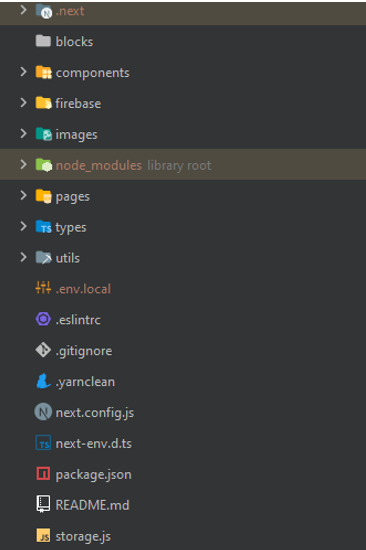
\includegraphics[scale=.45]{estrutura_next.png}
    \vspace{5pt}
    \legend{Fonte: Próprio autor}
\end{figure}

Por meio dos componentes, mostrados na estrutura da figura \ref{componentes} é possível a reutilização do código-fonte para diversos layouts, como, por exemplo, o componente NavBar, o qual é utilizado em diversas páginas, tornando-as padronizadas. Com isto, cada componente, também, terá seu estilo por meio de um arquivo de módulo do CSS, que estende os estilos globais, podendo sobrepô-los. Portanto, cada componente terá sua finalidade pré-definida, podendo ser reutilizada caso sirva o propósito.

\begin{figure}[H]
    \caption{\label{componentes}Estrutura dos componentes}
    \vspace{5pt}
    \centering
    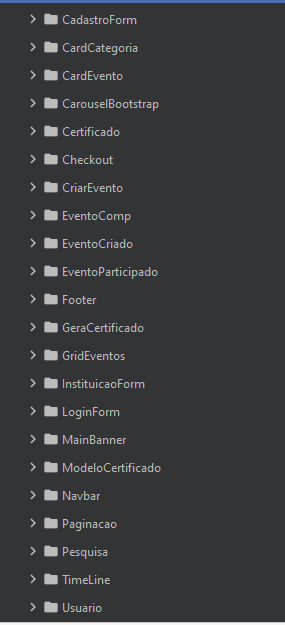
\includegraphics[scale=.45]{componentes.png}
    \vspace{5pt}
    \legend{Fonte: Próprio autor}
\end{figure}

\section{Rotas Next.js}
Em relação às rotas, serão as páginas a serem acessadas pelo usuário. Dito isso, estas deverão validar, caso necessário, se o usuário está logado por meio de uma requisição ao \textit{backend}. Além disso, estas devem requisitar diversas informações para poderem ser exibidas nas páginas e terem os dados necessários preenchidos de cada componente. Conforme estruturação presente na figura \ref{pages}, cada página tem seu nome e sua estruturação interna, podendo ter sub-rotas, que serão chamadas dentro da pasta. Esta regra vale para todas as pastas presentes, com exceção das 404 (a qual está destinada a páginas não encontradas, ou seja, caso seja digitada uma \textit{url} dentro do domínio que não seja pertencente a esta lista, irá a chamar, visto que é uma página customizada) e a 403 (que determina um recurso não possível de ser acessado para determinado usuário).
\begin{figure}[H]
    \caption{\label{pages}Estruturação de páginas no Next.js}
    \vspace{5pt}
    \centering
    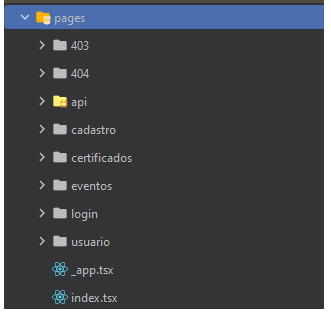
\includegraphics[scale=.6]{pages.png}
    \vspace{5pt}
    \legend{Fonte: Próprio autor}
\end{figure}

\section{Renderização das páginas}
Dentro das páginas da aplicação, diretamente do Next.js, foram utilizadas ambas as implementações de pré-renderização presentes no framework. Em páginas que podem ter cache, como, por exemplo, as páginas individuais de cada evento, principalmente por conterem diversas imagens, além de não necessariamente precisarem estar sendo constantemente atualizadas, sendo estas geradas em tempo de compilação, e tendo em vista que o evento nem seja editado, foi utilizado o método de \textit{Static Generation} com \textit{Incremental Static Regeneration}. Ou seja, por todas as páginas serem baseadas nos mesmos componentes, tendo sua diferença apenas os dados requisitados, foi criado um cache para cada um, gerando uma página HTML com um JSON de dados, para cada uma das páginas. Isto faz com que o acesso seja mais rápido, e o cache é de um minuto, ou seja, a cada um minuto se o evento for editado e caso haja uma requisição, a página será gerada novamente com base no que foi atualizado em cada uma das páginas desta rota dinâmica.

Há também a outra implementação de pré-renderização, sendo a \textit{Server-side rendering}, utilizada em páginas, como a de pesquisa dos eventos. A sua utilização se deve ao fato de que esta deve ser geradas constantemente baseada nos filtros que o usuário irá fazer dada a sua necessidade. A página é mais lenta em relação a uma geração estática, porém todo o processamento fica no servidor que está hospedada a aplicação, deixando com o navegador do usuário final apenas com o HTML gerado em tempo de execução dada essa frequência de atualização desta página, por exemplo.

% -----------------------------------------
\chapter{Resultados e discussões}\label{chp:LABEL_CHP_5}
\label{resultados}
% -----------------------------------------
Com a utilização de \textit{frameworks} modernos, foi possível criar uma aplicação web responsiva e fluida. Ao se comparar com o estado inicial, os mockups seguiram seus propósitos e com base neles, foi possível a criação de todas as telas do sistema, conforme visto no capítulo \ref{chp:LABEL_CHP_5}. A figura \ref{home} demonstra a tela inicial, que todas as pessoas irão visualizar ao entrar na aplicação. Comparada ao mockup, há uma maior riqueza de detalhes, assim como melhorias que puderam ser ajustadas. Seguindo para as telas de cadastro, como a de Login na figura \ref{login}, o fundo foi levemente alterado em sua paleta para corresponder ao que foi gerado anteriormente. 

\begin{figure}[H]
    \caption{\label{home}Página inicial}
    \vspace{5pt}
    \centering
    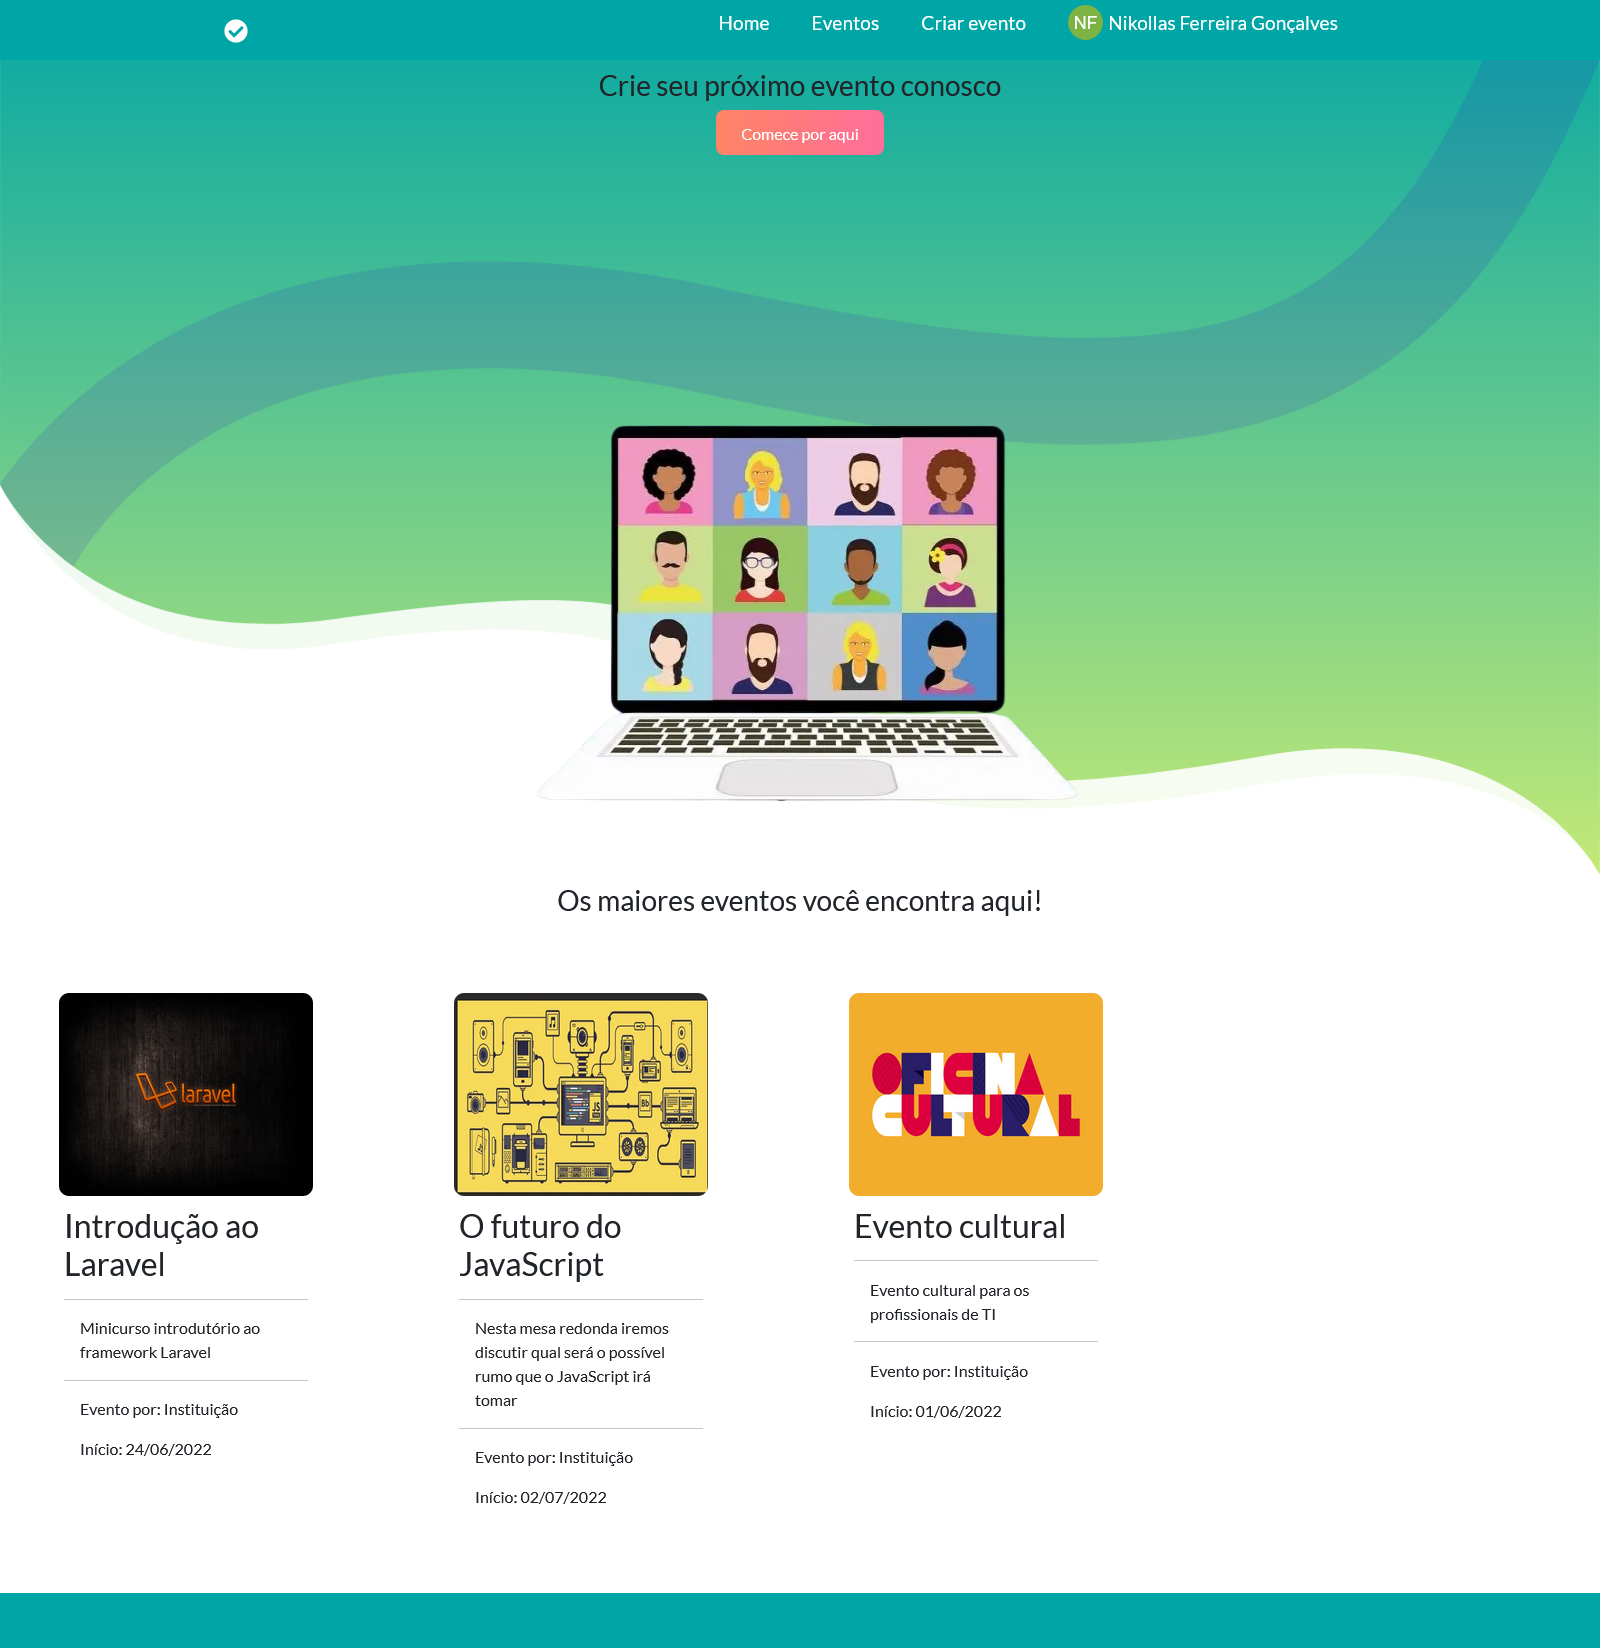
\includegraphics[scale=.23]{home.png}
    \vspace{5pt}
    \legend{Fonte: Próprio autor}
\end{figure}
\begin{figure}[H]
    \caption{\label{login}Página de login}
    \vspace{5pt}
    \centering
    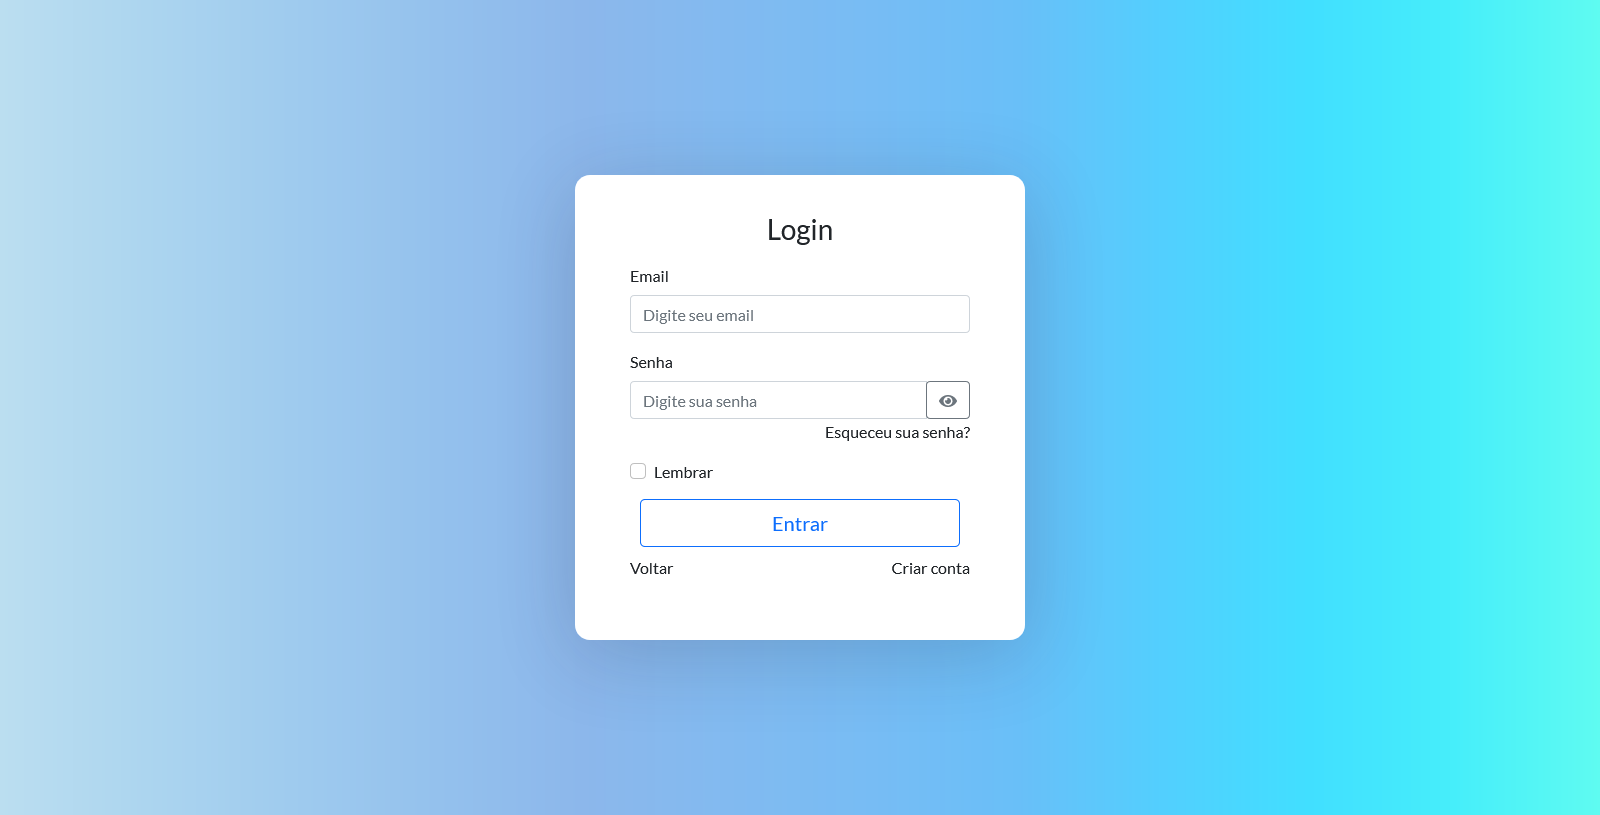
\includegraphics[scale=.25]{login.png}
    \vspace{5pt}
    \legend{Fonte: Próprio autor}
\end{figure}

Utilizando a página inicial como exemplo, é possível ver a responsividade adaptada a ela por meio das figuras \ref{homemob1} e \ref{homemob2}, que se adaptam a um smartphone. A diferença entre o tamanho de tela de um desktop para um smartphone fez com que a \textit{navbar} seja oculta e as imagens dos eventos sejam exibidas apenas uma por linha, dimensionando a imagem para isto.

\begin{figure}[H]
    \caption{\label{homemob1}Página inicial \textit{mobile}}
    \vspace{5pt}
    \centering
    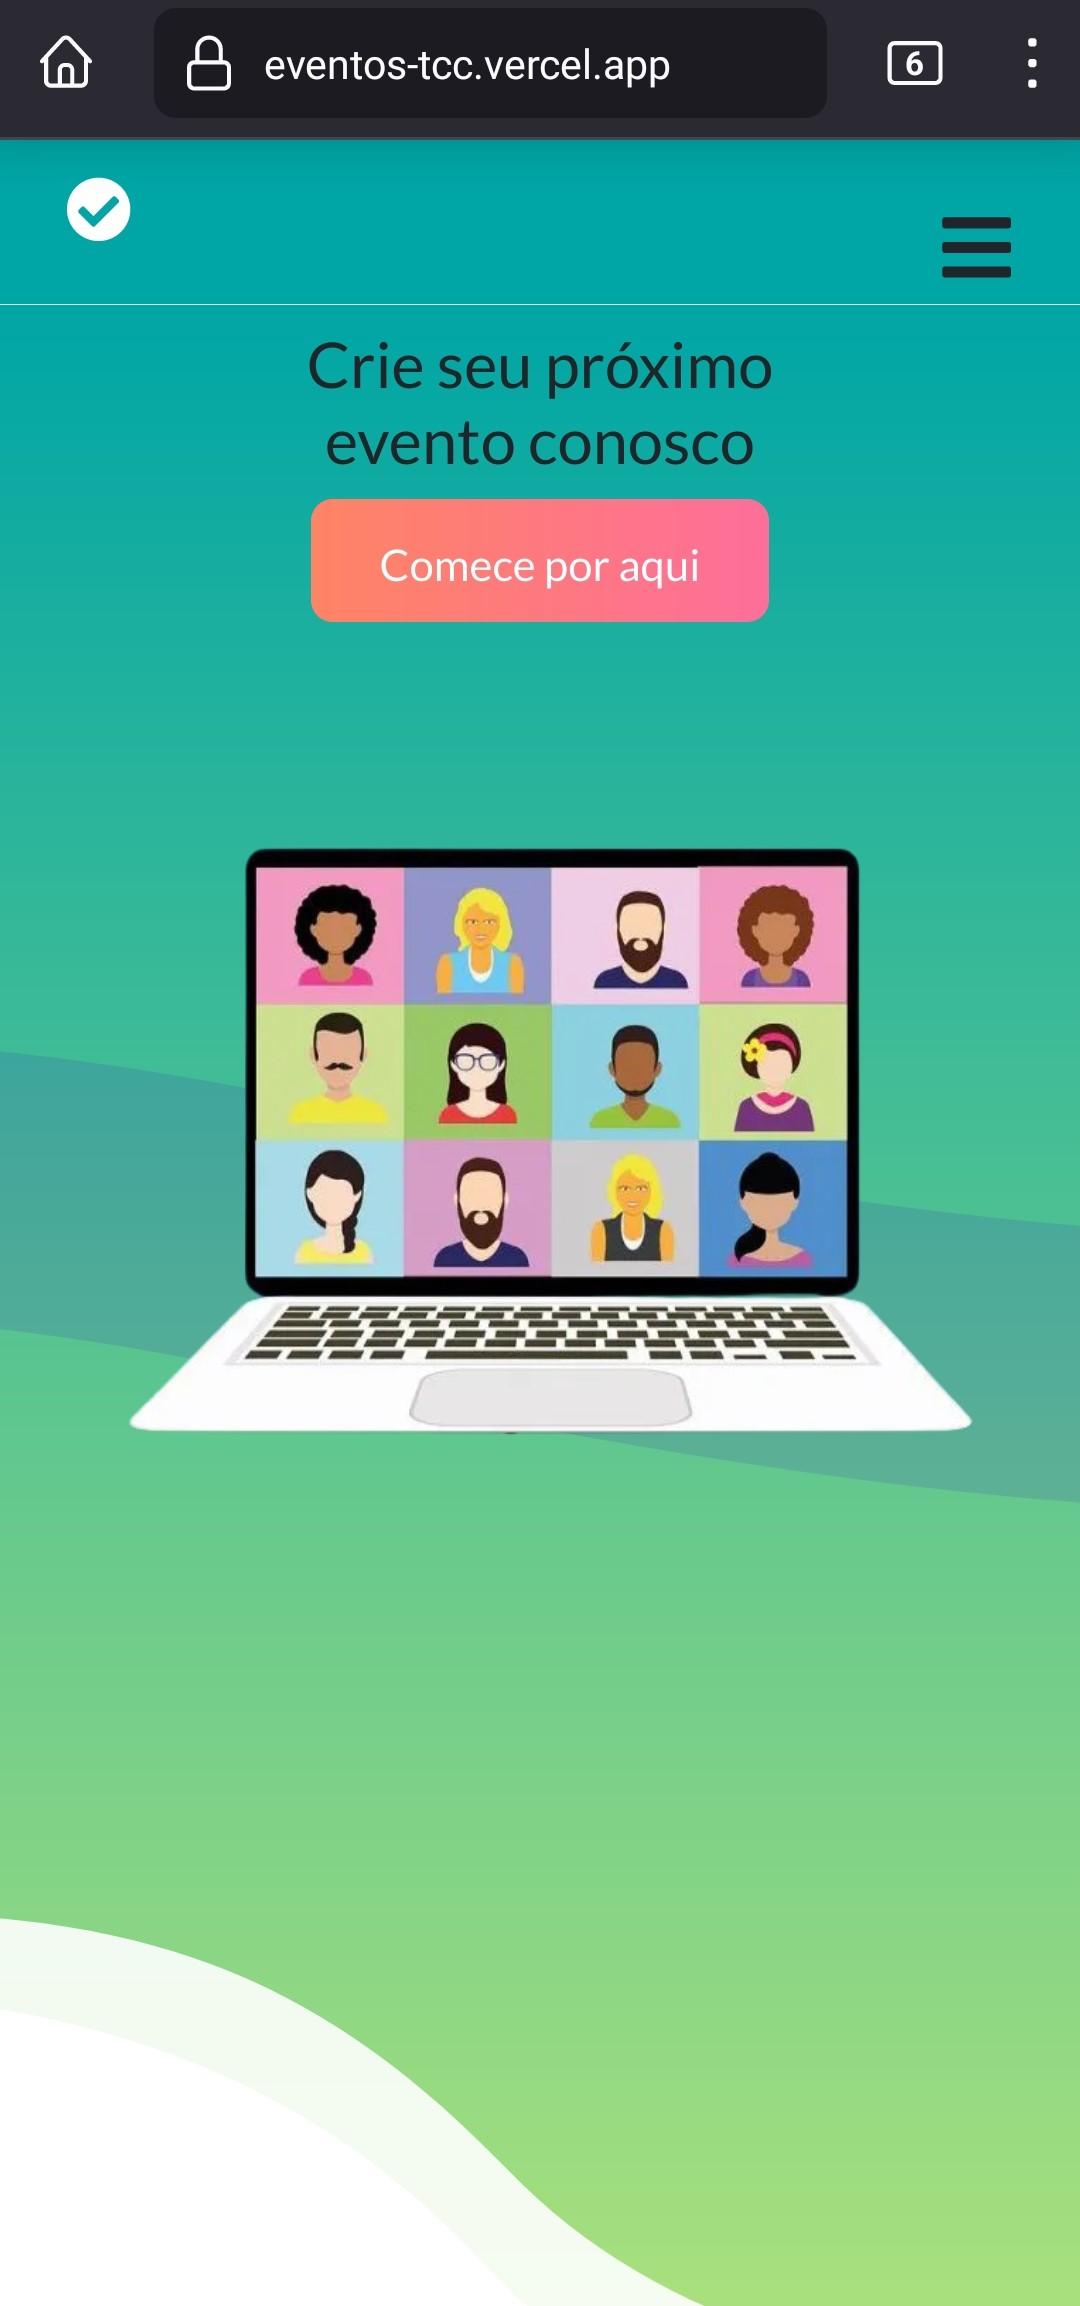
\includegraphics[scale=.15]{homemob1.jpg}
    \vspace{5pt}
    \legend{Fonte: Próprio autor}
\end{figure}

\begin{figure}[H]
    \caption{\label{homemob2}Continuação da página inicial \textit{mobile}}
    \vspace{5pt}
    \centering
    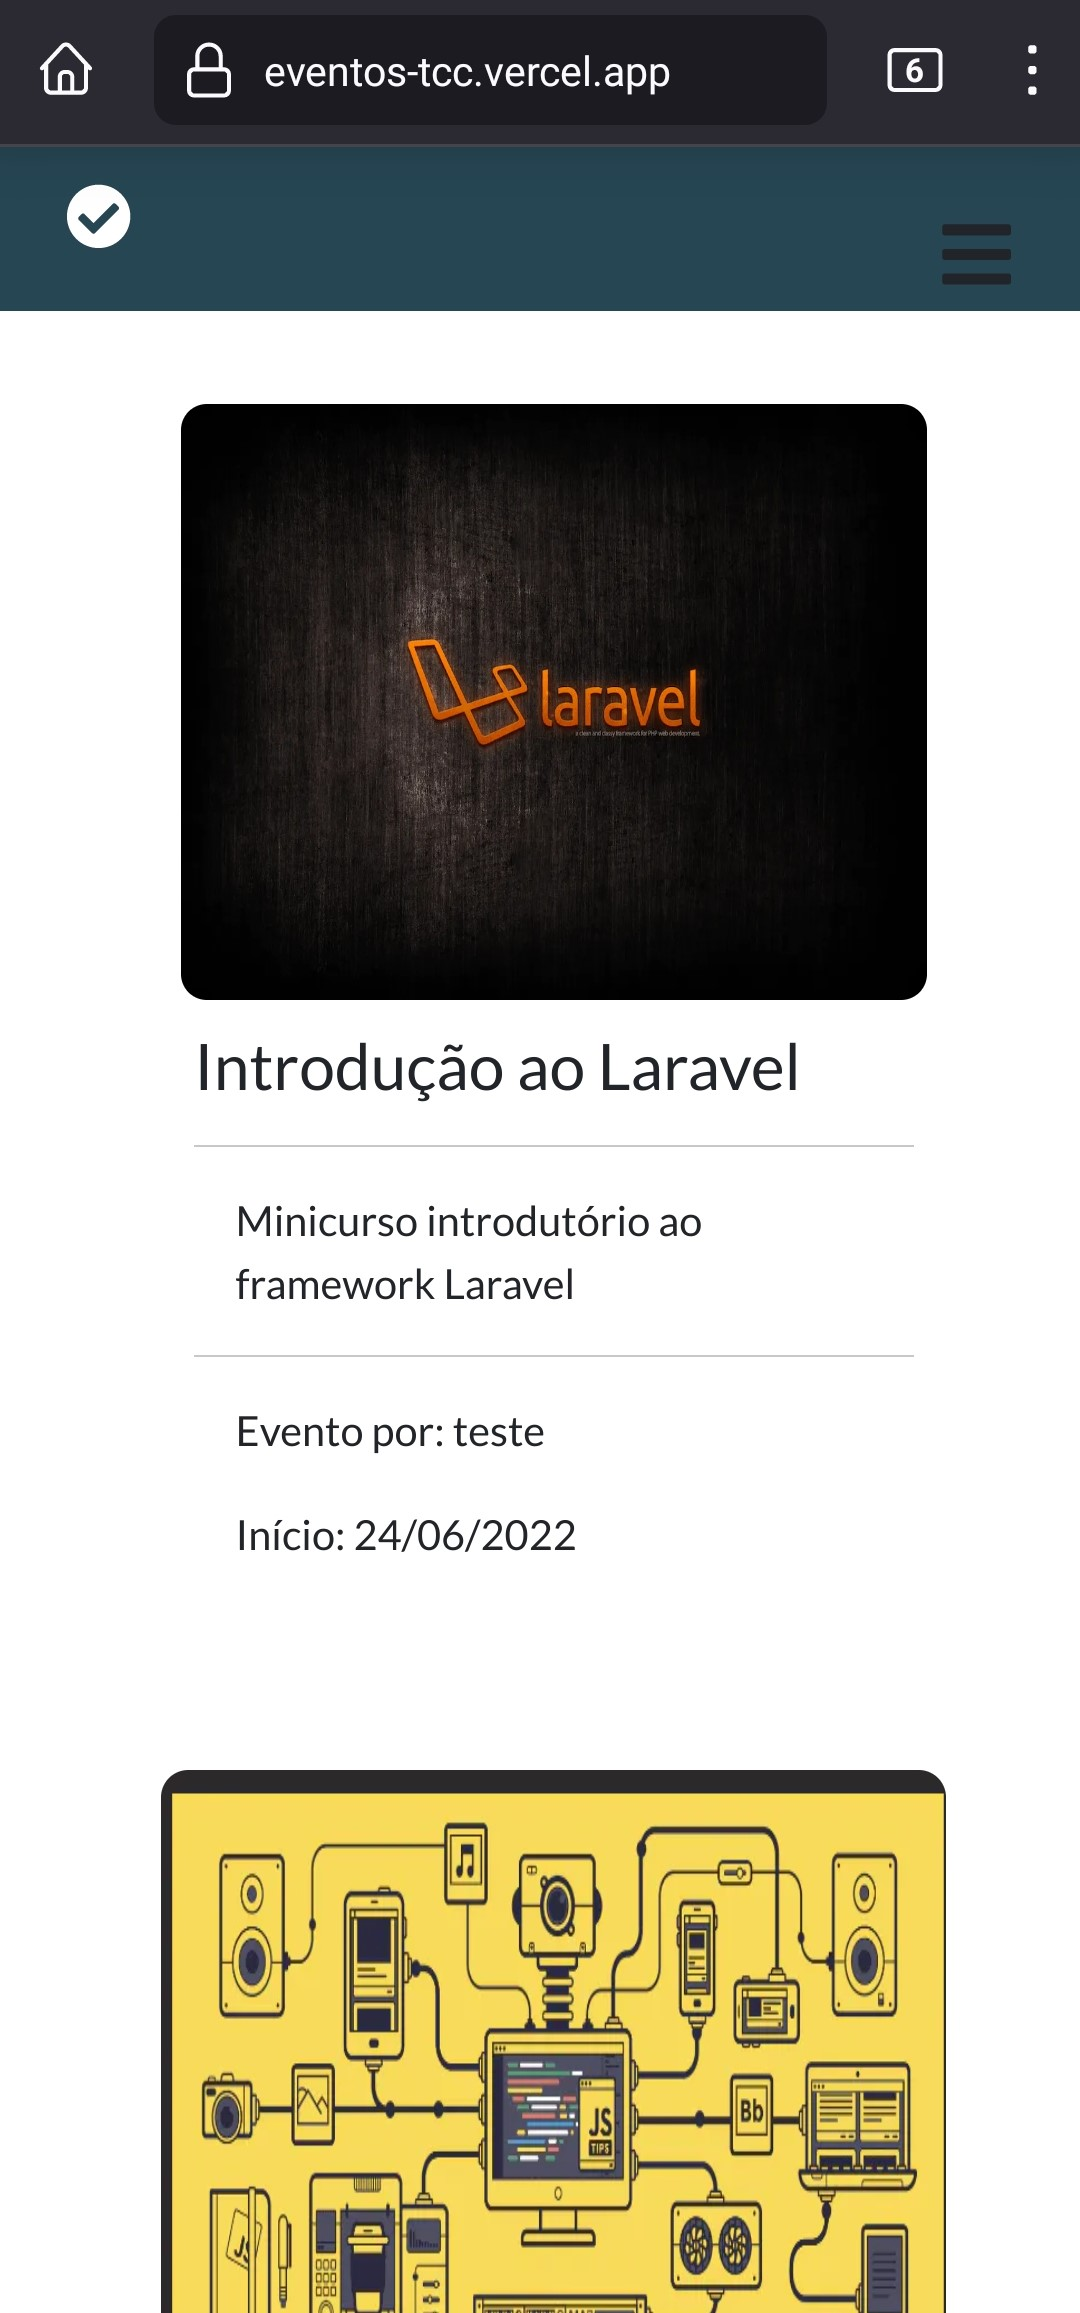
\includegraphics[scale=.15]{homemob2.jpg}
    \vspace{5pt}
    \legend{Fonte: Próprio autor}
\end{figure}

A fluidez, conforme as estatísticas capturadas pela Vercel, foi obtida por meio de carregamento rápido das páginas juntamente com a otimização de imagens fornecidas pelo framework Next.js. A imagem \ref{estVercel} demonstram os dados capturados e suas estatísticas disponíveis no plano gratuito, com o maior problema sendo a primeira impressão dos dados na tela(\textit{First Contentful Paint}), que demonstra o primeiro carregamento dos dados no cliente. Este resultado é esperado, devido ao cache do framework, armazenado em seu servidor após o primeiro uso, o que decai ao longo do tempo, devido a este fator.

\begin{figure}[H]
    \caption{\label{estVercel}Estatísticas Vercel \textit{mobile}}
    \vspace{5pt}
    \centering
    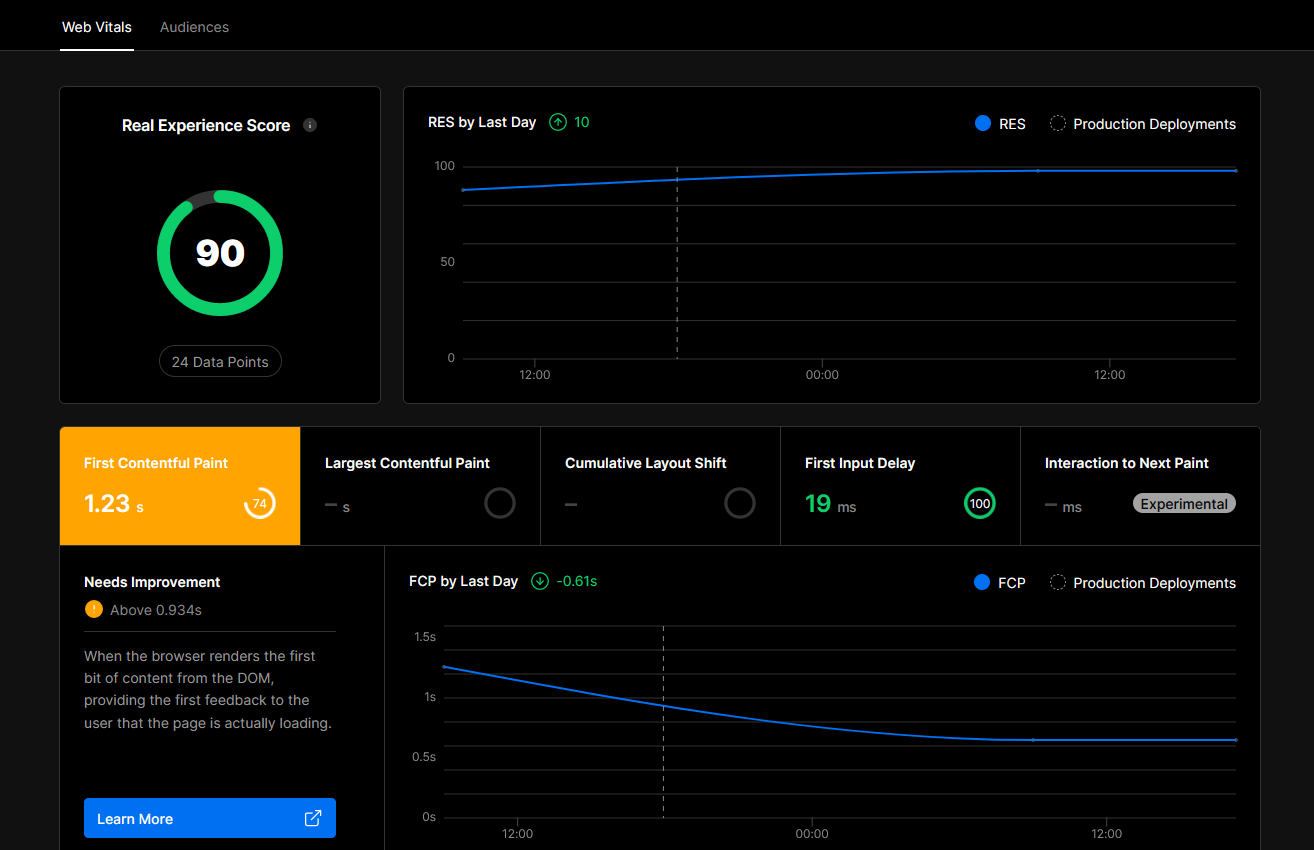
\includegraphics[scale=.3]{vercel_dados.png}
    \vspace{5pt}
    \legend{Fonte: Próprio autor}
\end{figure}

Foi criada uma exibição padrão para cada evento, seguindo o modelo de mockup. Com isto, a aplicação segue um modelo padrão para cada evento, modificando apenas as informações com as imagens contidas em cada um. Na figura \ref{evento}, é possível ver o detalhamento do evento em si e, com a figura \ref{atividades} (que estão na mesma página), tem-se completamente os dados para a participação do usuário, com a descrição completa de quem e o que será apresentado no evento. 

\begin{figure}[H]
    \caption{\label{evento}Página de evento}
    \vspace{5pt}
    \centering
    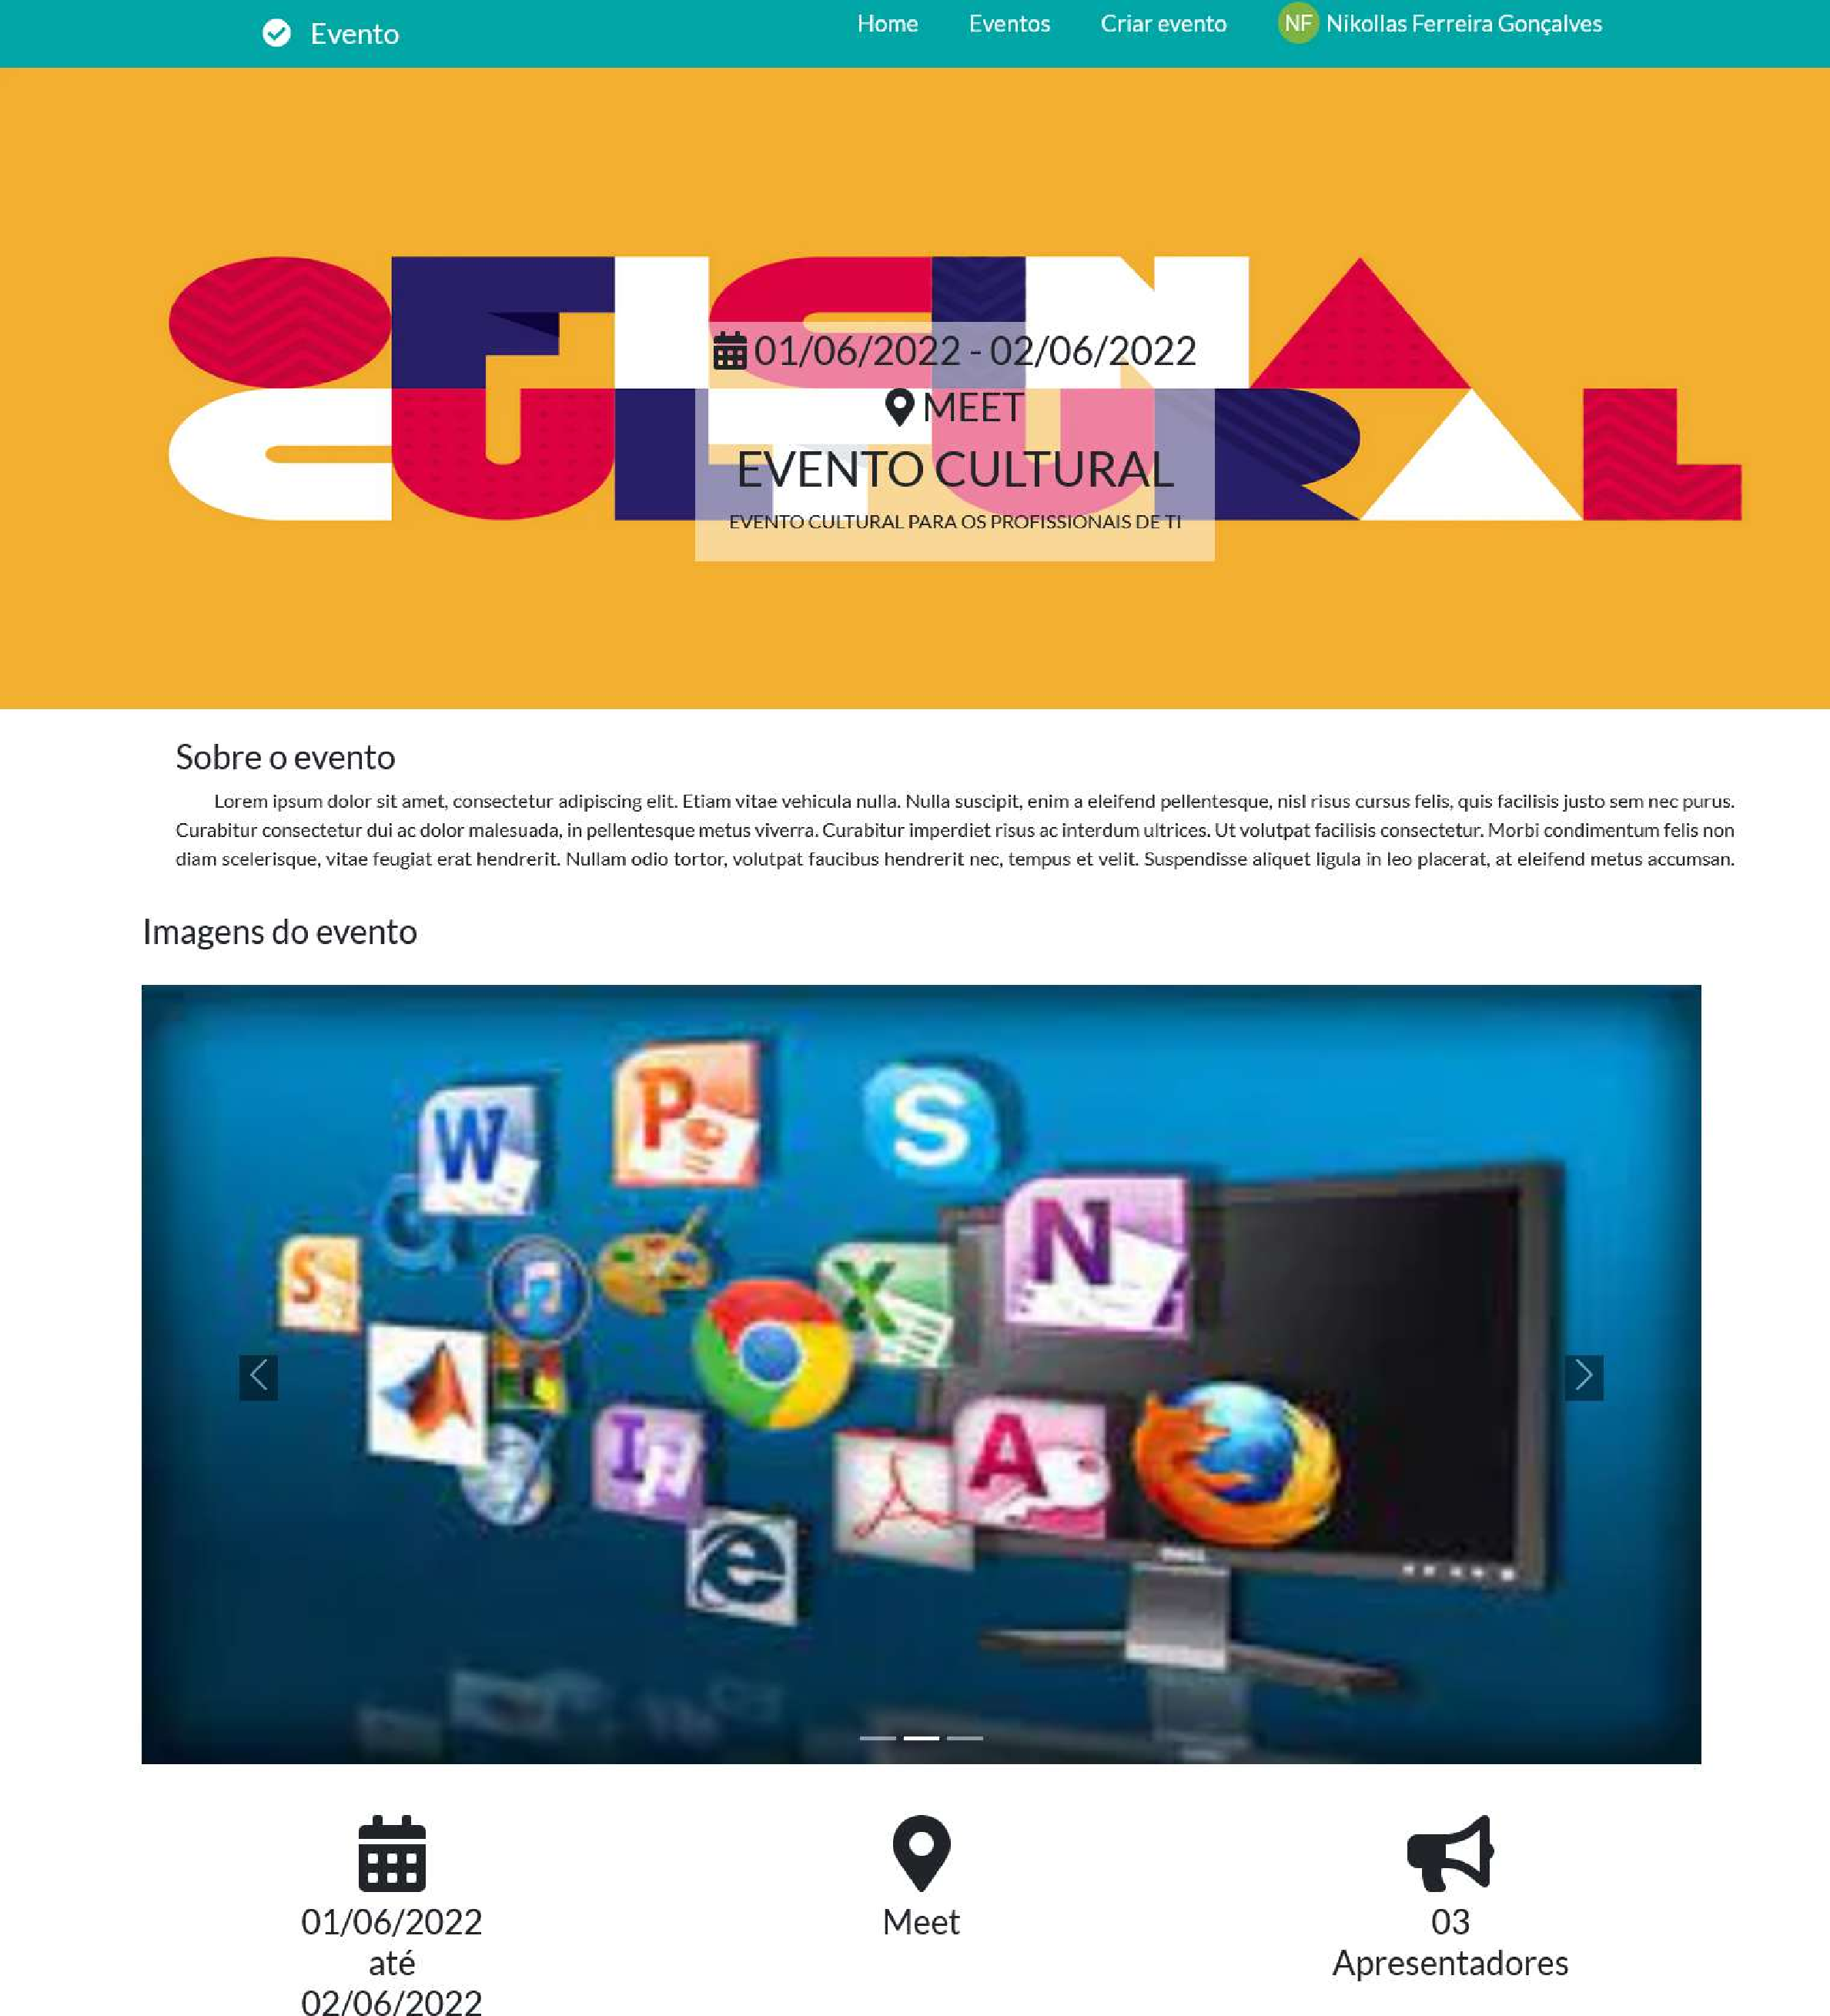
\includegraphics[scale=0.25]{evento.pdf}
    \vspace{5pt}
    \legend{Fonte: Próprio autor}
\end{figure}
\begin{figure}[h]
    \caption{\label{atividades}Atividades}
    \vspace{5pt}
    \centering
    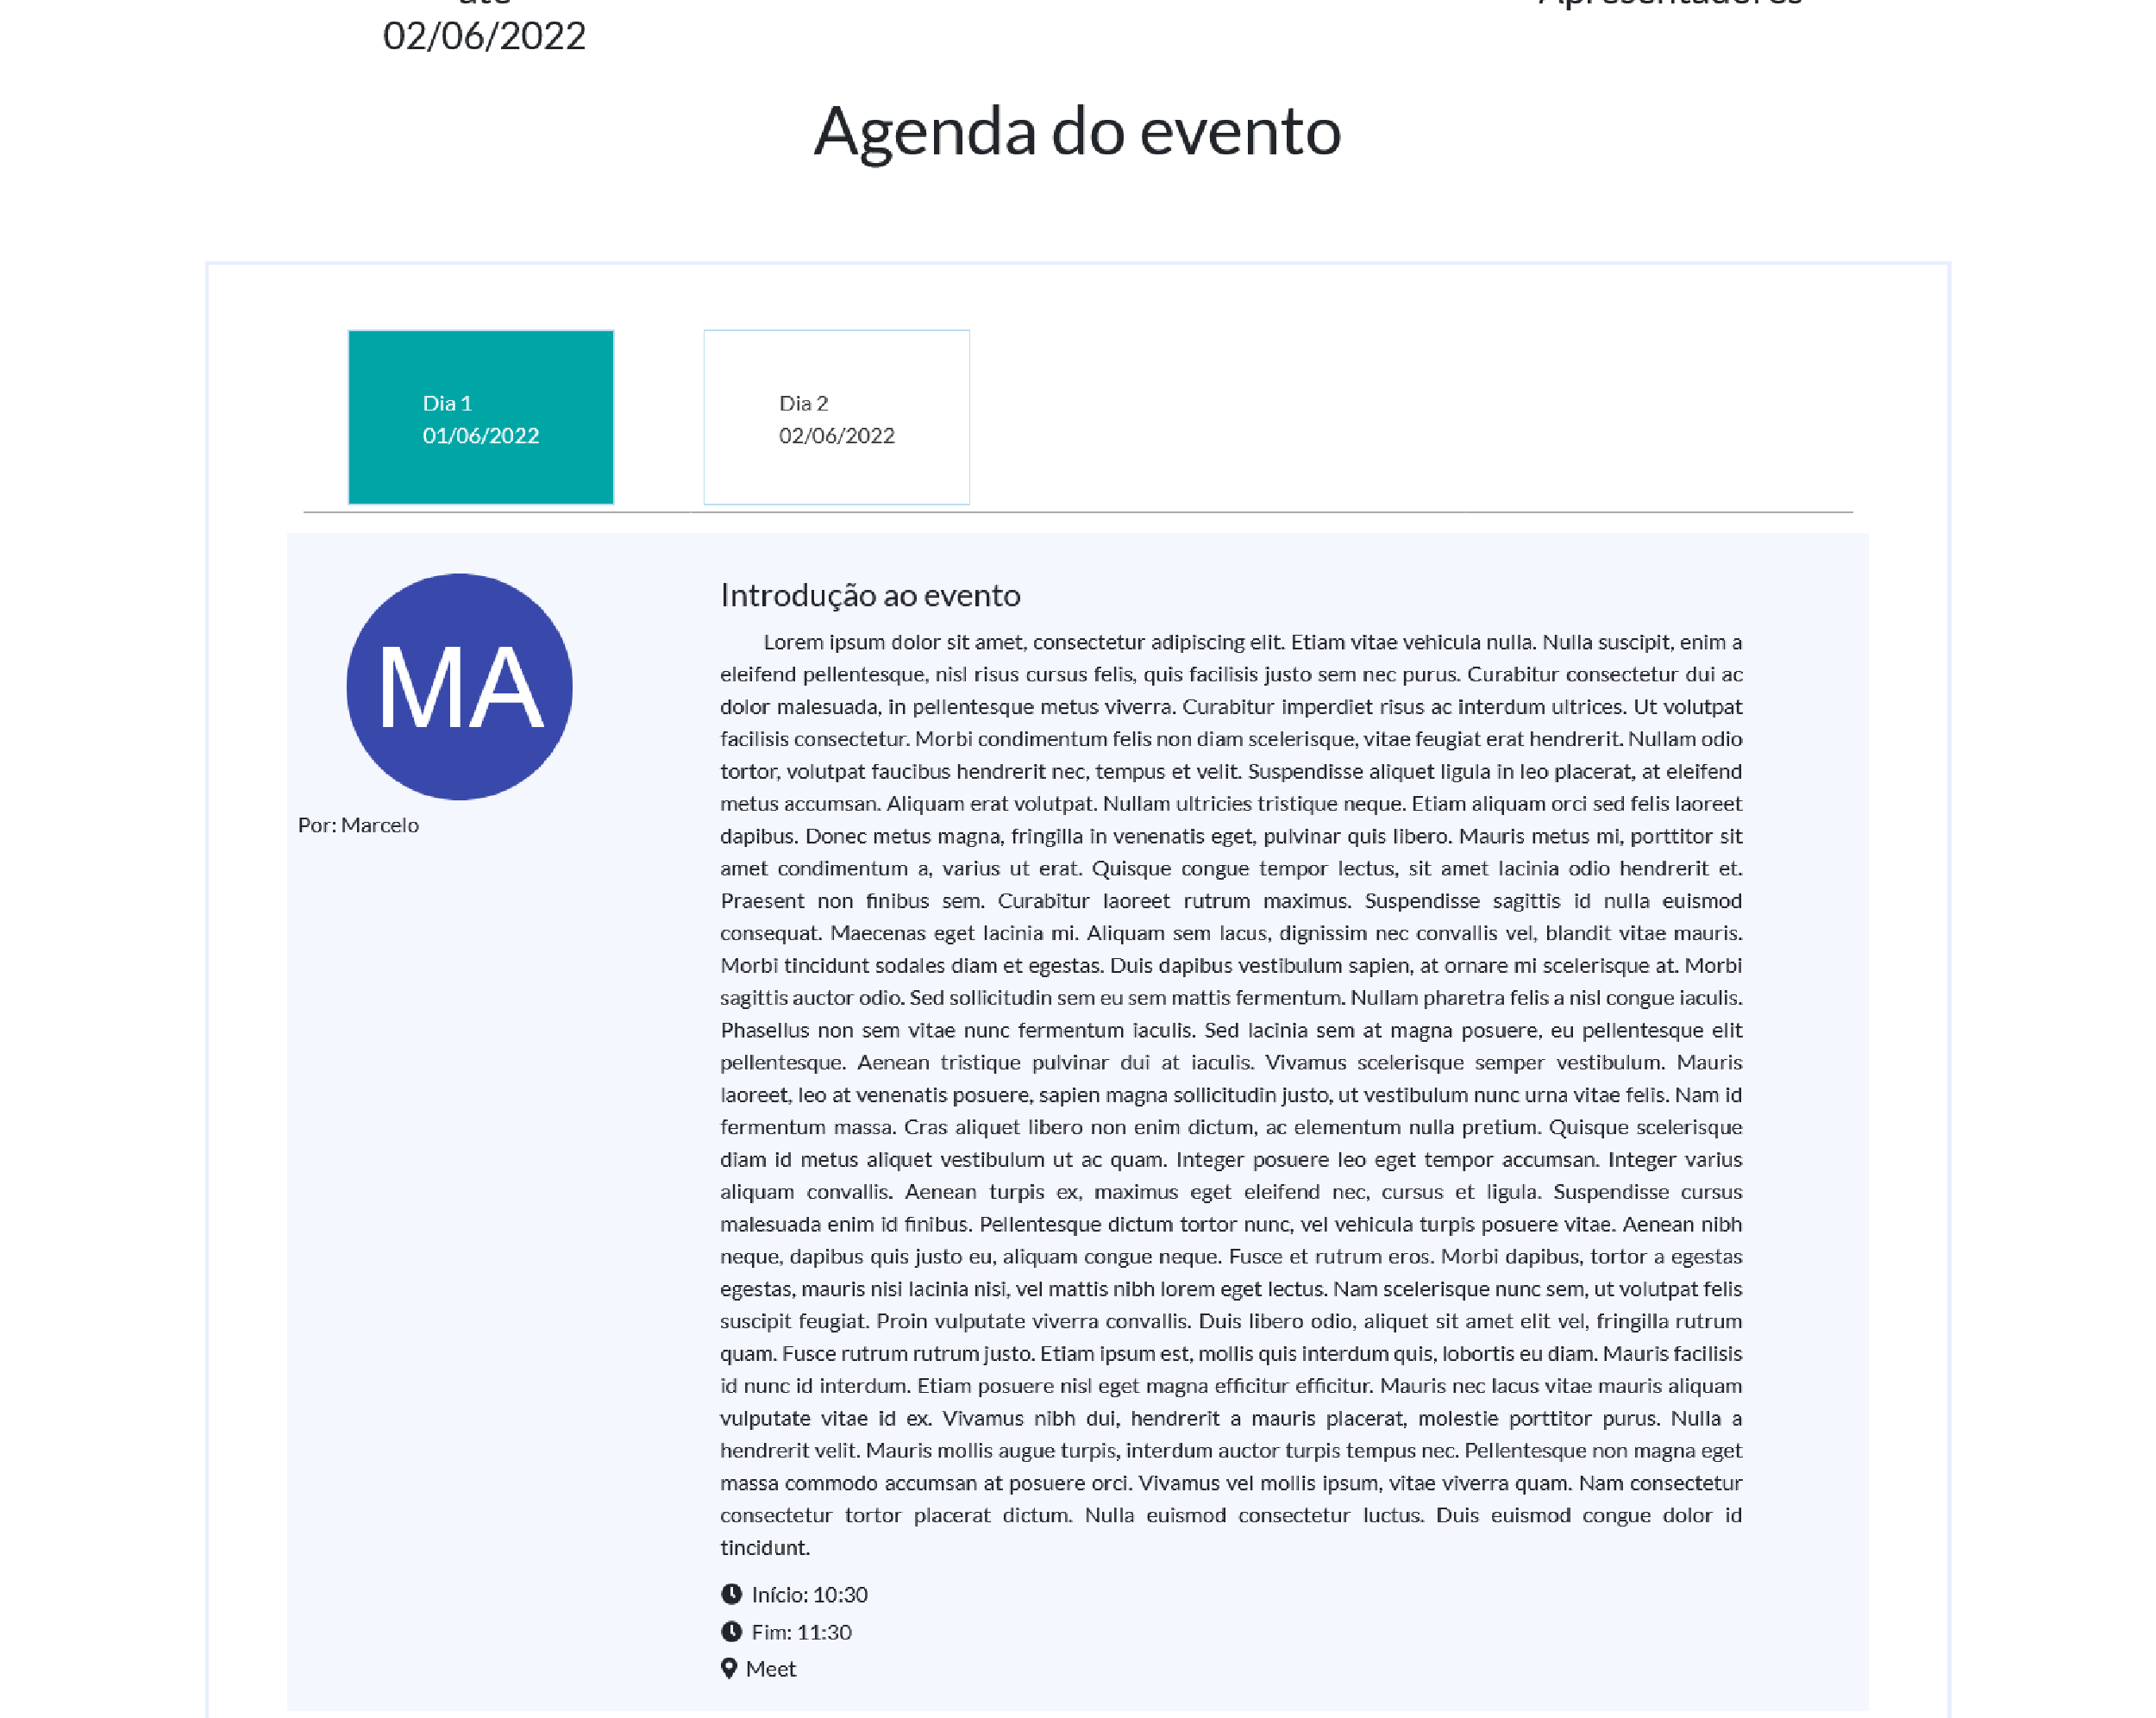
\includegraphics[scale=.25]{atividades.pdf}
    \vspace{5pt}
    \legend{Fonte: Próprio autor}
\end{figure}
%Seguindo para a tela de usuário, a qual será utilizada para gerenciamento de certificados, assim como de eventos, conforme previsto no mockup inicial, apenas alguns detalhes foram ajustados, como ajustes em alguns efeitos visuais de componentes da tela. Então, o que se altera são a quantidade de opções para cada uma das funções descritas anteriormente, como mostram a figura 21, figura 22 e a figura 23, sendo a primeira de um usuário comum, a segunda de um associado e a última de um administrador.\\
O modelo de certificado criado e que pode ser enviado em formato de PDF para o e-mail do participante, incluindo neste caso o apresentador também, também é gerido pela aplicação. Então, foi necessário criar um validador e enviar juntamente ao PDF o código para validação, como demonstrado na figura \ref{certificado}.

\begin{figure}[H]
    \caption{\label{certificado}Exemplo de certificado}
    \vspace{5pt}
    \centering
    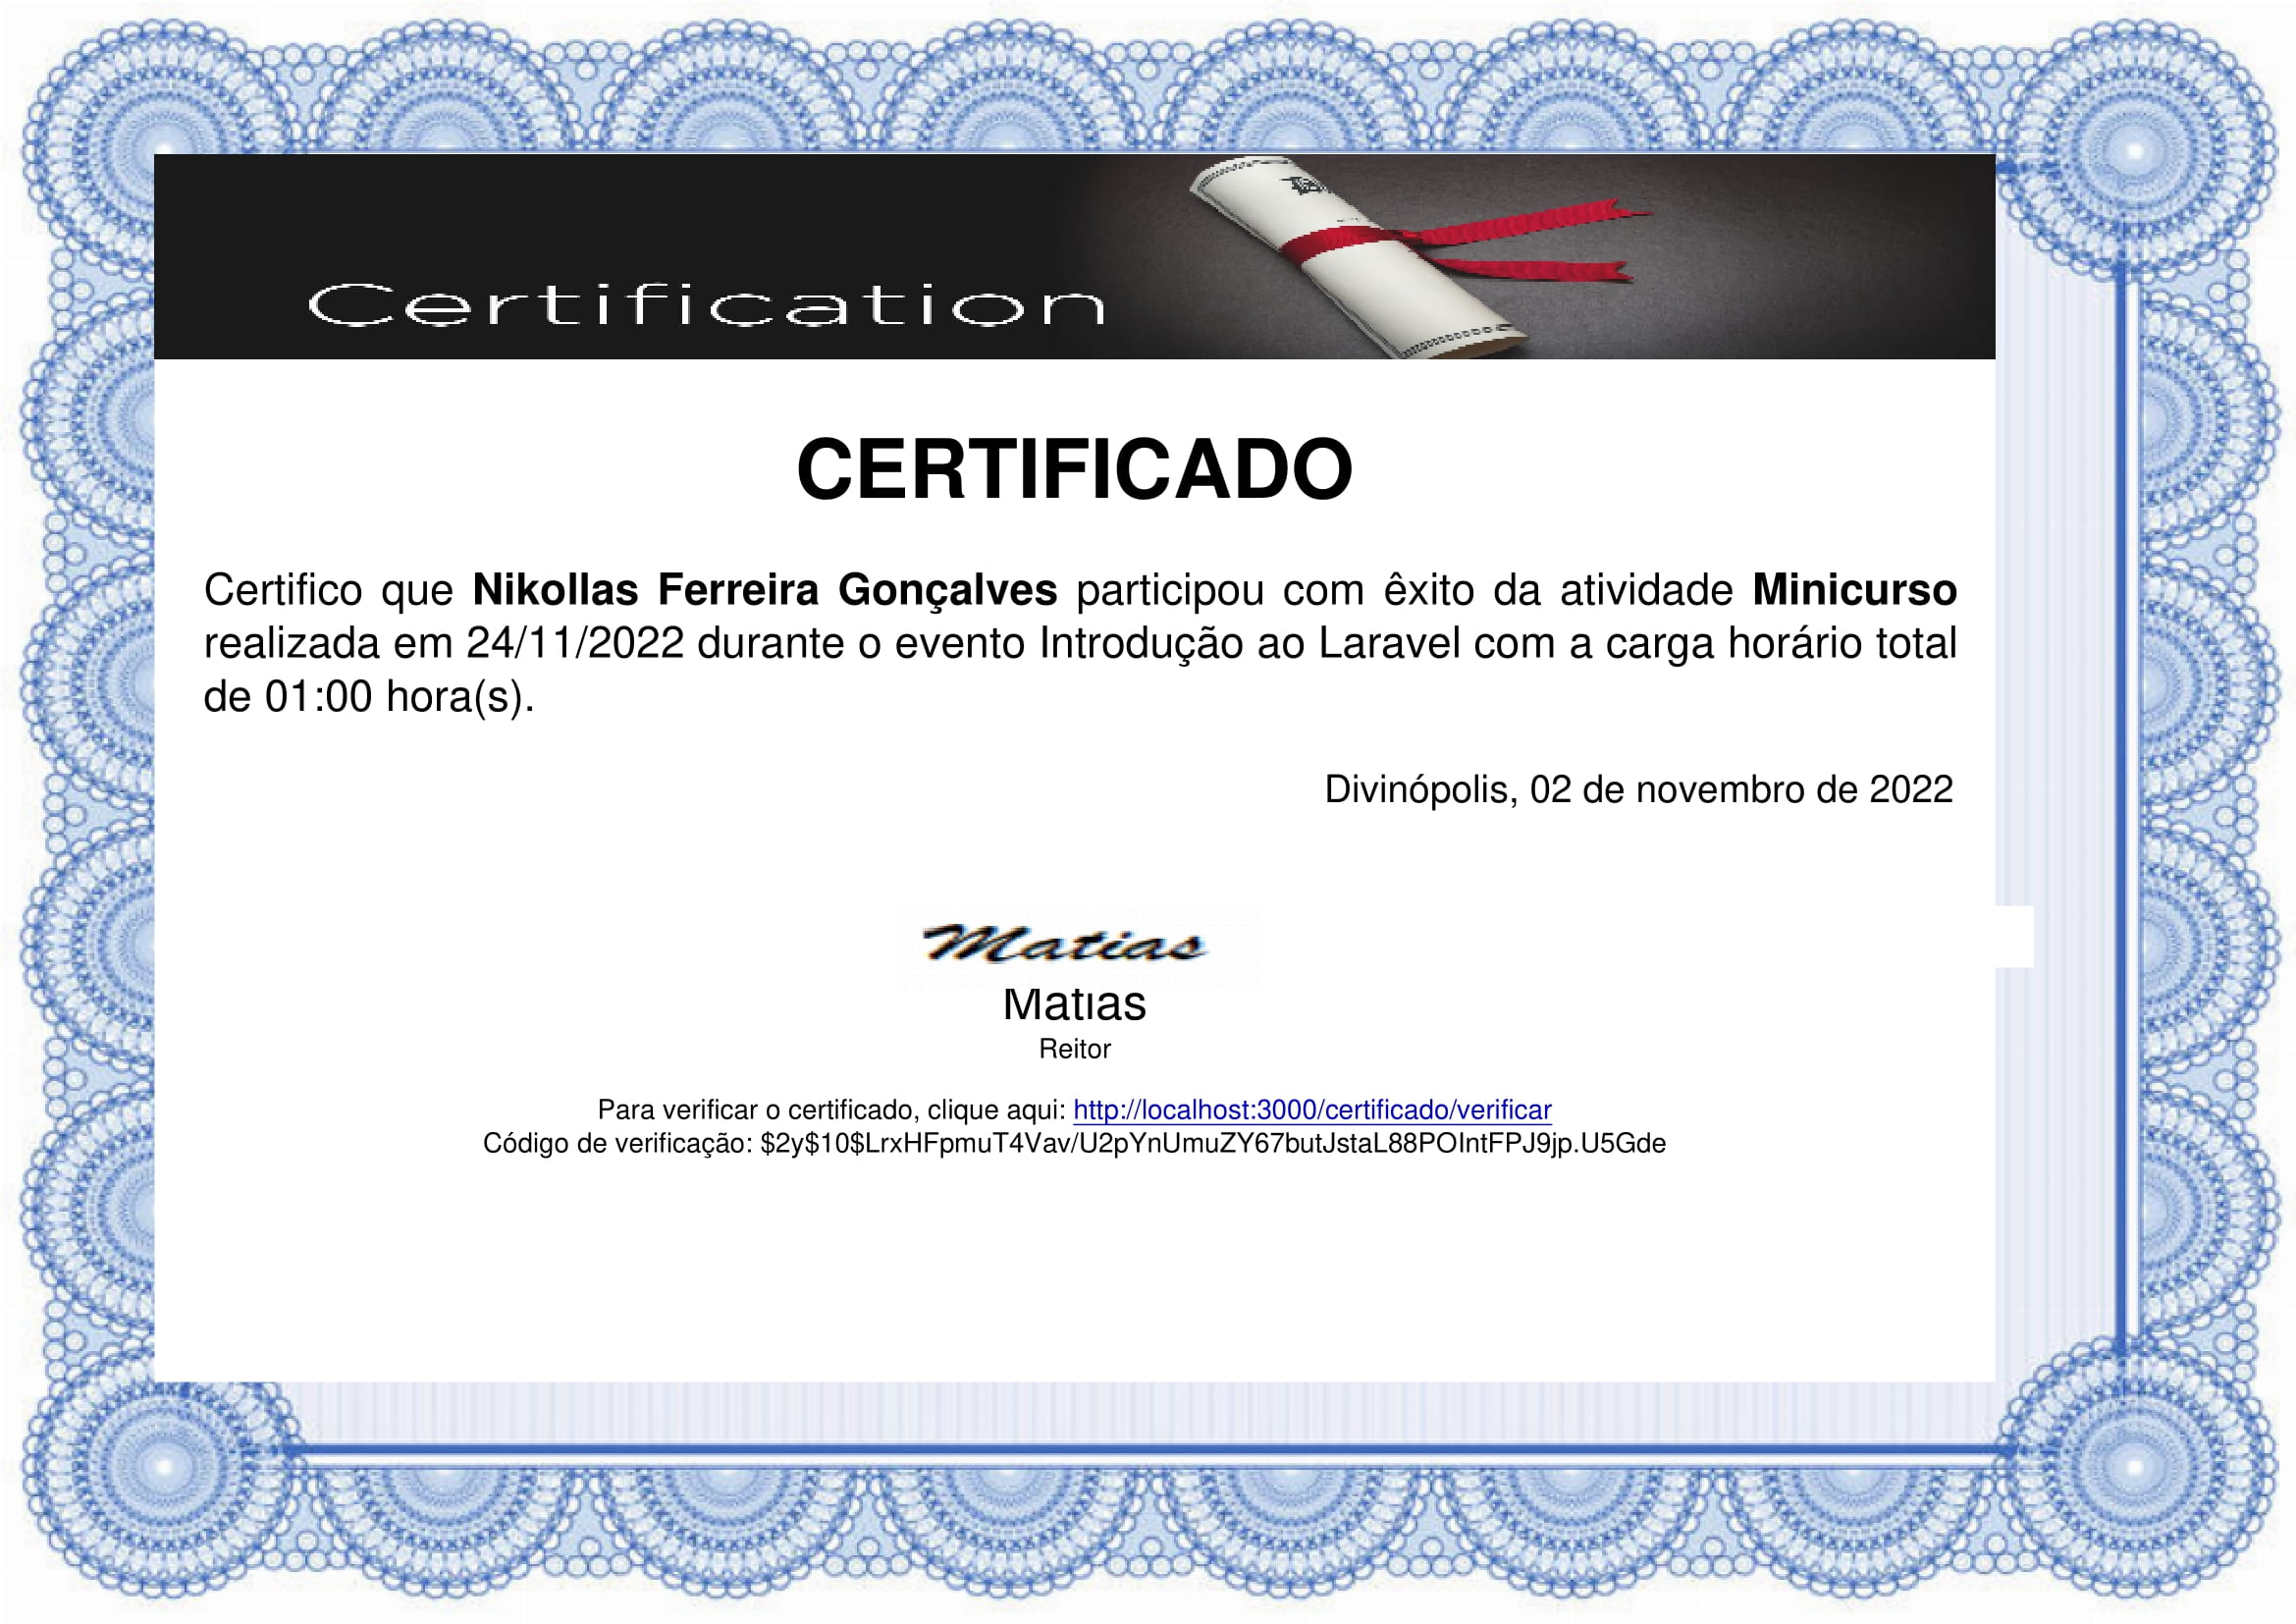
\includegraphics[scale=.20, angle=-90]{certificado-1.jpg}
    \vspace{5pt}
    \legend{Fonte: Próprio autor}
\end{figure}

A criação do \textit{backend} que foi realizada apresenta um token JWT para autenticação e validação dos dados do usuário, além de realizar toda a troca de informações por meio de sua API REST e envio de e-mails dos certificados. Neste, é proporcionado um ambiente e troca de informações seguros por meio das requisições feitas pelo Next.js. Além disso, toda a estruturação inicial planejada foi seguida, com exceções de tabelas auxiliares criadas pelo próprio framework Laravel para facilitar gravações de suas estatísticas e informações essenciais ele, ou seja, toda a cardinalidade das tabelas, assim como o projeto das requisições foi seguido conforme planejado anteriormente.

Por se tratar de um framework bem estruturado e organizado, com o Laravel, foi possível criar um padrão para o projeto que apresente funções bem determinadas e cumprindo o requisito de estarem em seu local, como os Controllers tendo as funções de comunicação com o banco de dados, assim como o retorno da requisição por meio de uma resposta em JSON, e as rotas chamando cada uma dessas funções para serem executadas. Portanto, isto facilitou o desenvolvimento, criando-se um padrão pré-determinado e podendo ser expandido ainda mais para projetos em maiores escalas.

O protótipo da aplicação apresenta uma estrutura bem subdividida, contendo o \textit{frontend} e o \textit{backend} estruturados pelos seus frameworks, podendo ser escalável.

A geração dinâmica dos certificados é uma característica relevante da aplicação que padroniza em uma instituição como podem ser seus documentos. Os modelos podem ser replicados ou diferentes para cada evento, podendo tornar padrão ou exclusivo para cada uso. A API permite a possibilidade de a criação de um aplicativo para \textit{smartphones} sem a necessidade de refazer ou reestruturar o \textit{backend}, devido à implementação de tecnologias como o JSON e ser acessível via protocolo HTTP. Os dados na API são protegidos por meio da autenticação fornecida pelo Laravel, ou seja, os dados da aplicação só serão repassados para quem estiver autenticado e com permissão de acesso a determinadas informações por meio do JWT daquele usuário, que tem prazo de validade. 

Neste capítulo, foram apresentados os resultados do protótipo desenvolvido. A aplicação é capaz do gerenciamento de eventos, criação e edição dos usuários, assim como geração e validação dos certificados. Pode-se agregar diversas outras funcionalidades a este projeto, dado os frameworks e linguagens utilizados, sendo um protótipo que pode ser viabilizado e implementado em diversas instituições para seu uso no gerenciamento destas tarefas. As funcionalidades estão disponíveis na seguinte URL: \url{https://eventos-tcc.vercel.app/}, o repositório contendo o \textit{frontend} está disponível em \url{https://github.com/NikFG/evento_front} e o repositório do \textit{backend} está disponível em: \url{https://github.com/NikFG/eventos_api}.

\chapter{Conclusão}\label{chp:LABEL_CHP_6}

Neste trabalho, foi desenvolvida e apresentada uma aplicação gerenciadora de eventos acadêmicos gratuitos online, que facilita a criação e a visualização para as instituições e para o participante.\\
O protótipo apresentado é capaz do gerenciamento de usuários, instituições e eventos, assim como a organização por três funções distintas de usuários. Somando essas características, há uma interface intuitiva que visa facilitar todos os processos para seus usuários, sejam apresentadores, participantes ou gerenciadores dos eventos. Há características similares aos apresentados na introdução, unindo características relevantes de cada um, e transformando-as num protótipo capaz de melhorar o gerenciamento dos eventos cadastrados.\\
A implementação deste sistema, inicialmente, pode ser feita em qualquer âmbito acadêmico, visto que abrange os mais variados tipos de eventos acadêmicos, podendo substituir, em caso de serem por meios digitais, o atualmente utilizado na instituição. Ou seja, a sua geração de certificados, a qual possibilita até mesmo a verificação e envio por e-mail, facilita todo o gerenciamento ao selecionar os participantes e apresentadores que de fato estiveram no evento.\\
Além disso, a utilização de novas tecnologias, como Next.js e Laravel, mostra que é possível criar uma aplicação moderna, com utilizações de boas práticas de programação além de estarem em frameworks que são recentes. Tal utilização, além de reforçar a segurança, melhoram o desenvolvimento do código, dado as facilidades que cada um apresenta, como por exemplo a criação de páginas estáticas e dinâmicas no Next.js e o Eloquent ORM do Laravel, que facilita as querys no SGBD, assim como facilita a migração entre SGBDs diferentes, caso seja necessário.\\
Portanto, estre trabalho poderá contribuir com as instituições que realizam recorrentemente tais eventos acadêmicos, podendo ser utilizado de maneira simples e eficaz.  E, devido aos frameworks e tecnologias utilizados neste projeto, a aplicação funciona de maneira responsiva, podendo ser utilizada, tanto em computadores de uso pessoal, como em dispositivos móveis sem que haja maiores problemas, como a perda de funcionalidades e quebras no layout.




\phantompart

% ----------------------------------------------------------
% ELEMENTOS PÓS-TEXTUAIS
% ----------------------------------------------------------
\postextual

% Referências bibliográficas
\bibliography{monografia.bib} %nome do arquivo *.bib
% Consulte o manual da classe abntex2 para orientações 
% sobre os seguintes tópicos opcionais:

%------------ Glossário

%------------ Apêndices
\begin{apendicesenv}
	\partapendices
	%\input{apendices/arquivo.tex}
\end{apendicesenv}

%------------ Anexos
\begin{anexosenv}
	\partanexos
	%\input{anexos/arquivo.tex}
\end{anexosenv}

% INDICE REMISSIVO
\phantompart
\printindex

\end{document}
\grid
